\documentclass[11pt,oneside,letterpaper]{article}
% \documentclass[9pt,lineno]{elife}

% graphicx package, useful for including eps and pdf graphics
\usepackage{graphicx}
\usepackage{grffile}
\usepackage{subfig}
%\DeclareGraphicsExtensions{.pdf,.png,.jpg}

% basic packages
\usepackage{color}
\usepackage{parskip}
\usepackage{float}
\usepackage{microtype}
\usepackage{url}
\usepackage[T1]{fontenc}
\urlstyle{same}

% \setkeys{Gin}{draft} %% draft mode

% \usepackage[hidelinks]{hyperref}
% \hypersetup{colorlinks=true,linkcolor=black,citecolor=black,urlcolor=black}

\usepackage{longtable}
\usepackage[]{algorithm2e}

% reference figures across documents
\usepackage{xr}
%\externaldocument{mers-structure_supp}

% text layout
\usepackage{geometry}
\geometry{textwidth=15cm} % 15.25cm for single-space, 16.25cm for double-space
\geometry{textheight=22cm} % 22cm for single-space, 22.5cm for double-space

% helps to keep figures from being orphaned on a page by themselves
\renewcommand{\topfraction}{0.85}
\renewcommand{\textfraction}{0.1}

% bold the 'Figure #' in the caption and separate it with a period
% Captions will be left justified
\usepackage[labelfont=bf,labelsep=period,font=small]{caption}

% review layout with double-spacing
%\usepackage{setspace}
%\doublespacing
%\captionsetup{labelfont=bf,labelsep=period,font=doublespacing}

% cite package, to clean up citations in the main text. Do not remove.
%\usepackage{cite}
\usepackage{natbib}
%\renewcommand\citepleft{(}
%\renewcommand\citepright{)}
%\renewcommand\citepform[1]{\textsl{#1}}

\usepackage{amsmath}

%\usepackage{lineno}
%\linenumbers

% Remove brackets from numbering in list of References
%\renewcommand\refname{\large References}
%\makeatletter
%\renewcommand{\@biblabel}[1]{\quad#1.}
%\makeatother

\usepackage{authblk}
\renewcommand\Authands{ \& }
\renewcommand\Authfont{\normalsize \bf}
\renewcommand\Affilfont{\small \normalfont}
\makeatletter
\renewcommand\AB@affilsepx{, \protect\Affilfont}
\makeatother

% comments
%\usepackage{ulem}
\definecolor{purple}{rgb}{0.459,0.109,0.538}
\def\tb#1#2{\sout{#1} \textcolor{purple}{#2}}
\def\tbc#1{\textcolor{purple}{[#1]}}
\def\gdc#1{\textcolor{blue}{[#1]}}

% symbols
% \newcommand{\chiSq}{\chi^{2}_{df}} %LM: ancient DNA? =P %GD: quite :)
% \newcommand{\dtmrca}{\Delta_\mathrm{TMRCA}}
% \newcommand{\undtmrca}{\delta_\mathrm{TMRCA}}
% \newcommand{\dspr}{d_\mathrm{SPR}}

%%% TITLE %%%
\title{\vspace{1.0cm} \LARGE \bf Genomic horizon}

\author[1$\ast$]{Gytis Dudas}
\author[1]{Trevor Bedford}

\affil[1]{Vaccine and Infectious Disease Division, Fred Hutchinson Cancer Research Center, Seattle, WA, USA}

\begin{document}

\maketitle

\begin{abstract}
Inexpensive pathogen genome sequencing has transformed the field of genetic epidemiology into genomic epidemiology.
Outbreak investigations have benefited the most from the inclusion of genome sites beyond short and rapidly evolving genes.
Despite the reduction in cost, pathogen genome sequencing has not seen universal adoption across pathogen-specific fields.
In this study we use a well-characterised Ebola virus dataset to show the differences in phylogenetic, temporal, and spatial resolution between complete genomes ($\sim$19kb long) and the rapidly evolving glycoprotein (GP) gene ($\sim$2kb long).
By quantifying errors in phylogenetic reconstruction we hope to persuade researchers looking to sequence pathogens during outbreaks of the utility of complete genome sequencing.
We further generalise our results by relating four parameters - probability, evolutionary rate, alignment length and waiting times - that determine how much information can be encoded by evolving pathogen lineages via mutations, which can help guide future sequencing studies.
\tbc{The use of `probability', etc... here is a bit opaque.'}
\end{abstract}

$\ast$ \footnotesize{Corresponding author (gdudas@fredhutch.org)}

\pagebreak

\section*{Introduction}
The combination of decreasing cost of sequencing and the unparalleled insight it offers have led to the adoption of pathogen genetic sequencing as one of the most effective tools in an modern epidemiologist's toolkit.
When coupled with sophisticated models of evolution, pathogen sequences can be used to look into epidemiological features such as cryptic transmission \citep{faria_establishment_2017}, migration \citep{dudas_virus_2017}, and origins \citep{smith_origins_2009} of infectious diseases, amongst others.
Pathogen sequences also contain information about past temporal dynamics beyond the time span over which sequences have been collected \citep{raghwani_origin_2012} owing to inheritance of mutations by future generations.

Molecular phylogenetic approaches rely on decoding these patterns of shared mutations into a nested data structure known as the phylogenetic tree.
\tbc{`Data structure' seems overly technical here.}
Population structure is often discernible in phylogenies, where specific lineages either arise via mutation or arrive from elsewhere and come to dominate within a particular demographic compartment (tissues, hosts, geographic areas, \textit{etc}.).
Pathogens often have short generation times and low replication fidelity (RNA viruses) such that mutations are generated at a rapid pace \citep{drummond_measurably_2003,biek_measurably_2015}, thus differentiating lineages genetically as they spread.
With appropriate sampling and information (``metadata'') about sequences, historic population dynamics can be inferred and quantified from pathogen phylogenies.
\tbc{This paragraph shoul be a bit more general than just about `population structure'. Recommend to cover `population dynamics', of which `population structure' is a part.}

Before widespread adoption of high-throughput sequencing limitations and costs led to amplification and sequencing of short fragments of pathogen genomes \citep{jin_genetic_1999,jin_proposal_2005}.
These subgenomic fragments were often chosen for their diversity, like viral surface glycoproteins evolving neutrally or under diversifying selection, or their utility, such as resistance profiling for HIV \textit{pol} \citep{kaye_phylogenetic_2008,rhee_human_2003}.
Whilst subgenomic fragments of pathogens are very accurate and specific as diagnostic markers, their length (dictated by the compromise between information content and ease of sequencing) limits their utility in detailed molecular epidemiology investigations \citep{wohl_co-circulating_2018}, as only mutations occurring with the small region of the genome are available for phylogenetic inference.

Mutations, prior to the action of selection, occur randomly across a genome via misincorporation of nucleotides during replication by the polymerase.
Many of these mutations are filtered out by selection if they adversely affect protein function, with leftover mutations being beneficial, neutral, or mildly deleterious.
Generally, neutral pathogen variation at the nucleotide level ebbs and flows with population demography but still outnumbers beneficial variation that tends to fix rapidly.
Mutations are often modelled as a Poisson process \citep{yang_computational_2006}, and the waiting time $t$ for observing a mutation at a single site is exponentially distributed with evolutionary rate parameter $R$.
Thus, the probability of observing 0 mutations at a single site after time $t$ is $e^{-Rt}$ and the probability of at least one mutation is $1-e^{-Rt}$.
Higher evolutionary rates \textit{R} or waiting times \textit{t} result in higher probabilities of observing at least one mutation.
Since sites are treated as evolving independently, the probability of observing a mutation across more than one site is related to the number of sites \textit{L} under observation
\begin{equation}
  P = 1-e^{-RLt},
\end{equation}
where \textit{RL} is expressed in substitutions per year.
Under a given evolutionary rate \textit{R}, probability of a mutation p, and sequence length \textit{L}, we can rearrange the equation to quantify the waiting times for mutations:
\begin{equation}
  t = \frac{log(P)}{-RL}
\end{equation}
\tbc{Feels unnecessary and I'd just express this via the mean waiting time.}.
When the evolutionary rate \textit{R}, sequence length \textit{L}, or probability of observing a mutation p are low waiting times are lengthened and vice versa.
Since both maximum plausible evolutionary rates and genome length are dictated by deleterious mutation load \citep{gago_extremely_2009}, neither quantity will vary substantially for a given pathogen, especially viruses \tbc{$RL$ won't vary substantially, though $R$ or $L$ individually might. Think of bacteria here.}.
Because of these natural constraints there is thus a lower limit to how many mutations can be expected to occur in a given length of sequence evolving at a particular evolutionary rate.
The mean waiting time for a mutation is easily calculated as 1/\textit{RL}.
We refer to this mean waiting time as the temporal horizon, which reflects a theoretical temporal resolution over which mutations arise and are available for phylogenetic inference in a system.

We use this study to argue in favour of sequencing complete pathogen genomes in outbreak scenarios where lineages need to be tracked at a fine scale.
We base our argument on the fact that pathogen genomes have an inherent mutation/temporal resolution limit which is already substantial for fine scale epidemiology and that sequencing subgenomic fragments of a pathogen results in loss of information that can make sequence data unreliable beyond diagnostics and typing.
We rely on a subset of a well characterised dataset of Ebola virus genomes from West Africa collected in 2014-2015 \citep{dudas_virus_2017}.
By analysing both complete viral genomes and the same dataset reduced to just the surface glycoprotein GP (corresponding to roughly 10\% of all available sites), we show substantial loss of predictive power, incorrect or unreliable reconstructions of past events, and migration model, despite increased evolutionary rate in GP compared to complete genome.
We hope that analyses presented in this study serve as a guide for researchers doing genetic epidemiology and will be of interest to model developers too.

\begin{figure}[h]
 \centering
	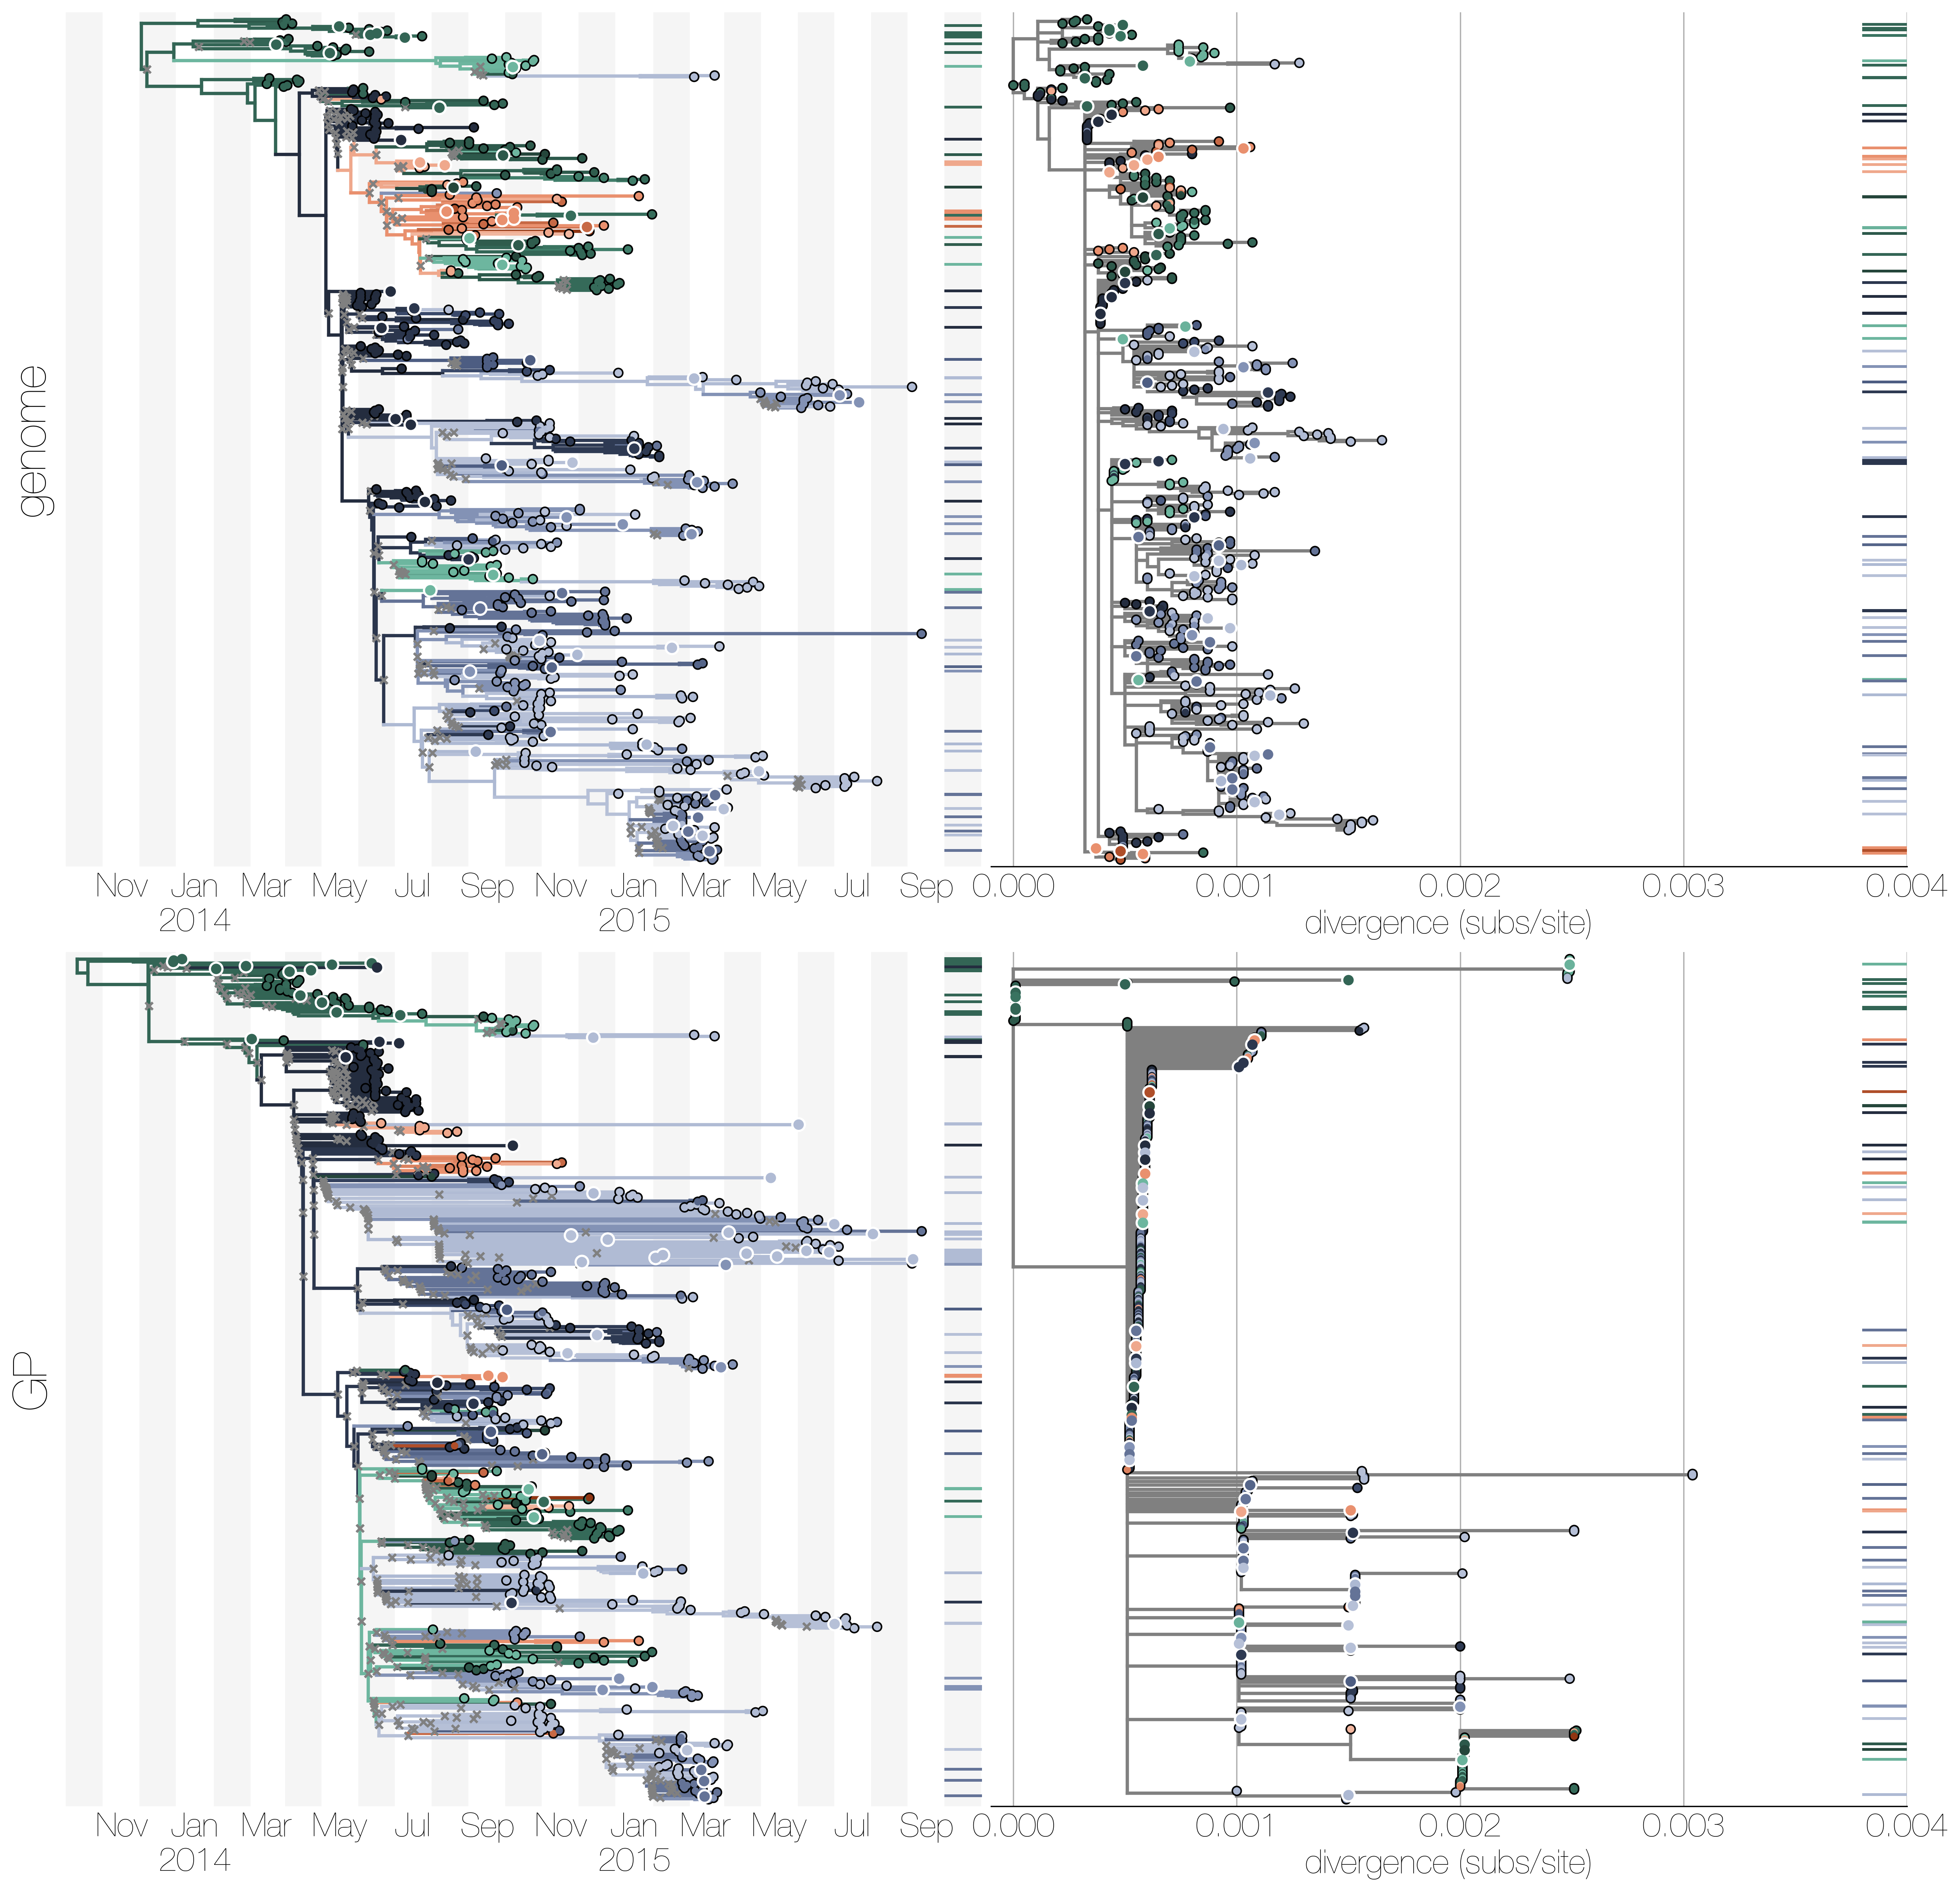
\includegraphics[width=0.75\textwidth]{figures/fig1_trees.png}
	\caption{\textbf{Phylogenies of West African Ebola virus genomes (top) or GP sequences (bottom).}
	Temporal phylogenies recovered using BEAST are shown on the left, maximum likelihood phylogenies recovered with RAxML are on the right.
  Tips are coloured based on country (Sierra Leone in blue, Liberia in red, Guinea in green) and location (lighter colours indicate administrative divisions lying towards west of the country).
  Tips outlined in white indicate the 60 chosen for date and location masking.
  In temporal phylogenies branches are also coloured based on GLM-inferred ancestral locations.
  Nodes in temporal phylogenies with <0.10 posterior probability are indicated with grey X marks.
  Maximum likelihood phylogenies on the right are rooted via temporal regression in TreeTime.
  \tbc{I see why you mirrored x-axis in right hand panels, but this seems to make genome divergence look \textit{less} than GP divergence. I'd make these x-axes independent so that top right has axis of 0 to $\sim$0.002.}
  \tbc{Also helpful to label the columns as `Time' and `Divergence'}.
	}
	\label{trees}
\end{figure}

\section*{Results}

\subsection*{Loss of phylogenetic signal}
In the past amplifying smaller fragments of pathogen genomes was often a pragmatic compromise between the cost of sequencing and information content, leading to sequencing of short but rapidly evolving pathogen genes or genomic regions.
What few sequences were available were often collected months apart or across large geographic areas, ensuring that many sequences were genetically distinct either via mutations occurring in the intervening time or through prior population differentiation.
However, in outbreak scenarios shorter genome fragments often do not accumulate mutations at a pace rapid enough to be of much use over short timescales.

Fig \ref{trees} shows the reconstructed phylogenies in substitution space (right) and time space (left) for 600 complete Ebola virus genomes (top) or just GP sequences (bottom).
Although higher levels of divergence are observed in the GP dataset, as seen from tree height, the differences in the number of non-polytomic nodes between genomic and GP data are clear, indicating substantially better resolution in disentangling the exact relationships between lineages in the former.
Internal branches of a phylogeny correspond to hypotheses of common ancestry and in the case of GP only 42 internal nodes are identified in the maximum likelihood phylogeny compared to 210 internal nodes for complete genomes.
Similarly, broad aspects of the West African epidemic can be inferred from both GP and genome phylogenies, such as Ebola virus' origins in Guinea, but the details of how it spread onwards are largely lost in the GP phylogeny.

Unlike maximum likelihood phylogenies where branch lengths are directly proportional to the expected number of substitutions, branch lengths in temporal phylogenies are usually smoothed out by the fact that a range of dates are compatible with a given number of mutations on a branch.
Thus even large polytomies can be resolved into a branching structure derived from the tree prior, albeit without much support for any given configuration.
This can be seen in Fig \ref{trees}, where temporal phylogenies (left) appear to have similar degrees of resolution, yet the GP dataset (bottom) contains more nodes with less than 0.10 posterior support (marked by grey crosses).
Similarly, there is a noticeable degree of branch clustering by country in the GP temporal phylogeny, possibly caused by proximity of locations within country, which in the absence of genetic information cannot be resolved to the same degree as with genomic data.

\begin{figure}[h]
 \centering
	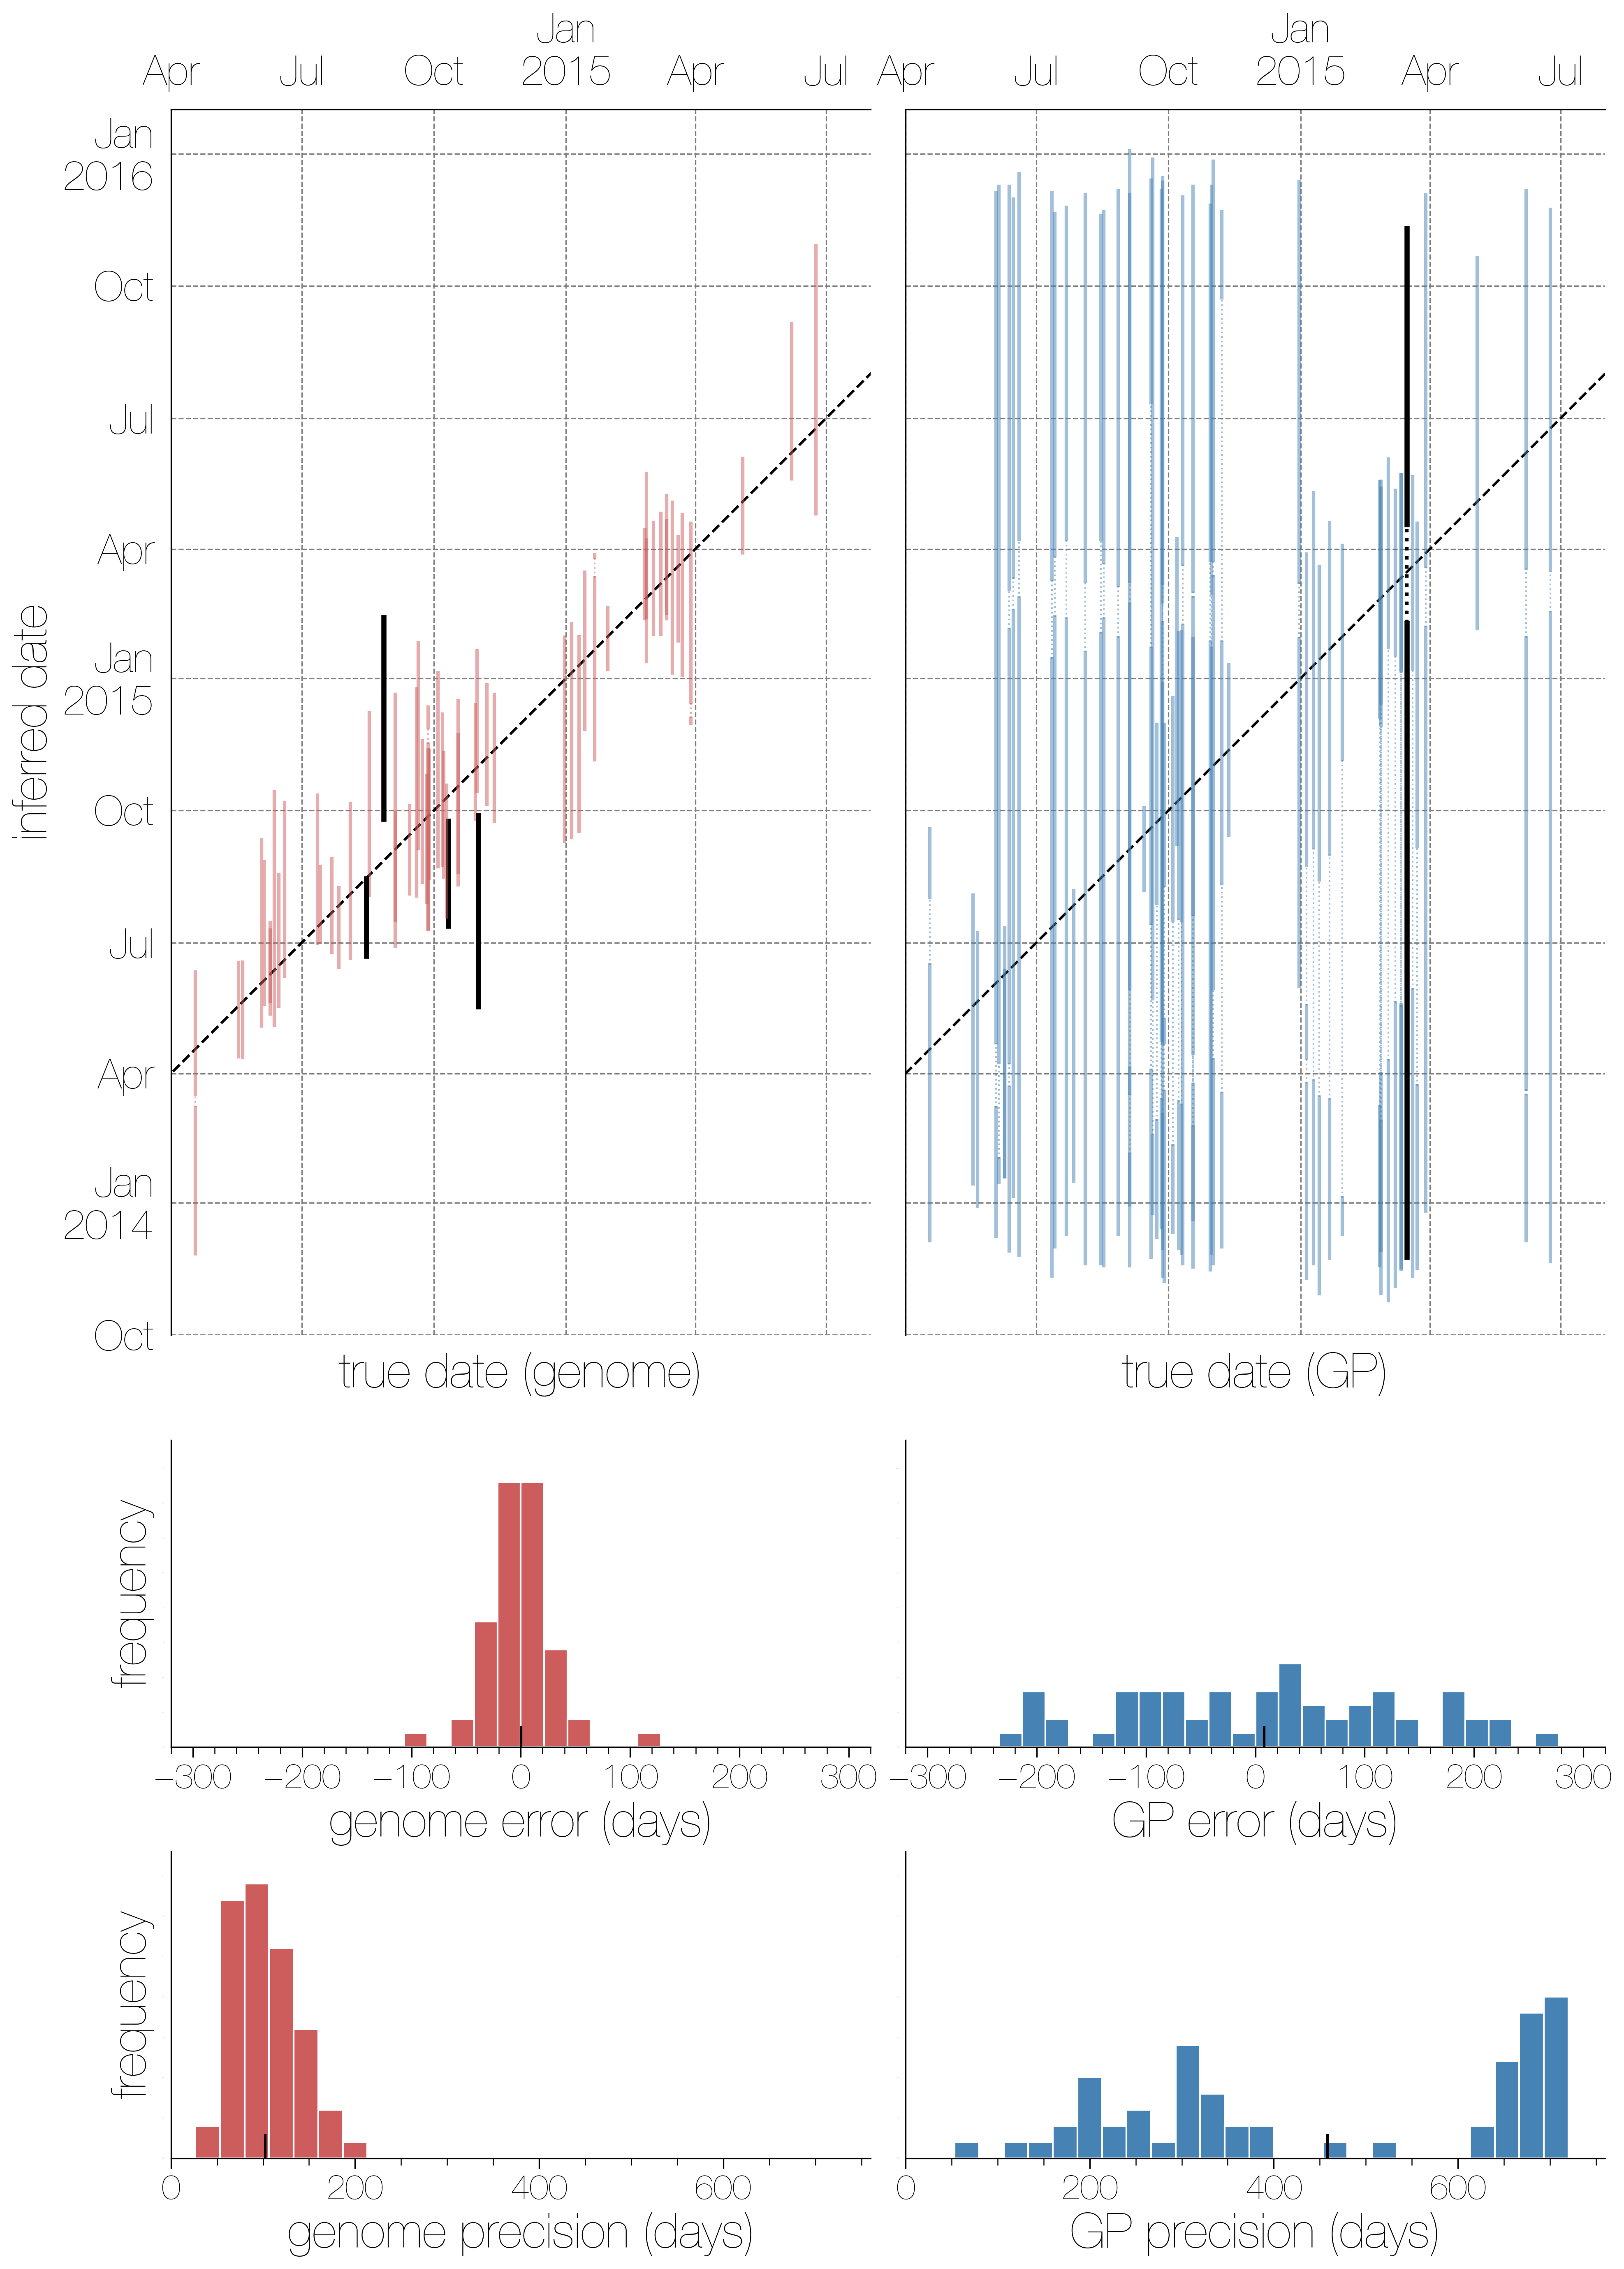
\includegraphics[width=0.75\textwidth]{figures/fig2_dates.png}
	\caption{\textbf{Masked tip date inference from genomes (left) and GP sequences (right).}
  Inferred collection dates in the masked set based on genomes (red, left) and GP sequences (blue, right).
  Each vertical line corresponds to the 95\% highest posterior density for the inferred tip date (y-axis), coloured red (genome) or blue (GP) if it falls within the true collection date (x-axis) and black otherwise.
  Dashed diagonal line indicates the 1-to-1 line.
  Posterior distributions of residuals from the 1-to-1 line are shown at the bottom with the mean of the distribution indicated by a tick mark.
	}
	\label{dates}
\end{figure}

\subsubsection*{Loss of temporal information}

Inferring masked tip dates from 10\% of the sequences (Fig \ref{dates}) is possibly one of the most intuitive ways to show both the noisiness of molecular clock estimates, as reflected in the width of 95\% highest posterior density intervals for inferred dates, but also the differences between GP and genome alignments.
True collection dates for genomes are mostly (56 out of 60) within the 95\% highest posterior density of estimated dates \tbc{refer to thhis as measuring the `coverage probability'}, and the absolute posterior error is around 0.081 years, corresponding to $\sim$1.0 month of error across all masked tips.
\tbc{Also report the average width of the individual CIs.}
The 95\% HPDs for inferred dates in the GP dataset, on the other hand, manages to capture more of the true dates (58 out of 60) at the cost of markedly reduced precision, with absolute posterior error going up to 0.417 years or $\sim$5.0 months.
\tbc{Also report the average width of the individual CIs.}
Absolute error for both genome and GP datasets is relatively close to theoretical expectations: one month versus predicted 3 weeks for genomes, and 5 months versus expected 3-6 months.
\tbc{How did you get these predictions? I think should include this calculation in Introduction.}
For many tips in the GP dataset independent Markov chains converged onto different dates for masked tips (\textit{i.e.} local maxima) resulting in multi-peaked posterior samples after combining independent analyses.

\begin{figure}[h]
 \centering
	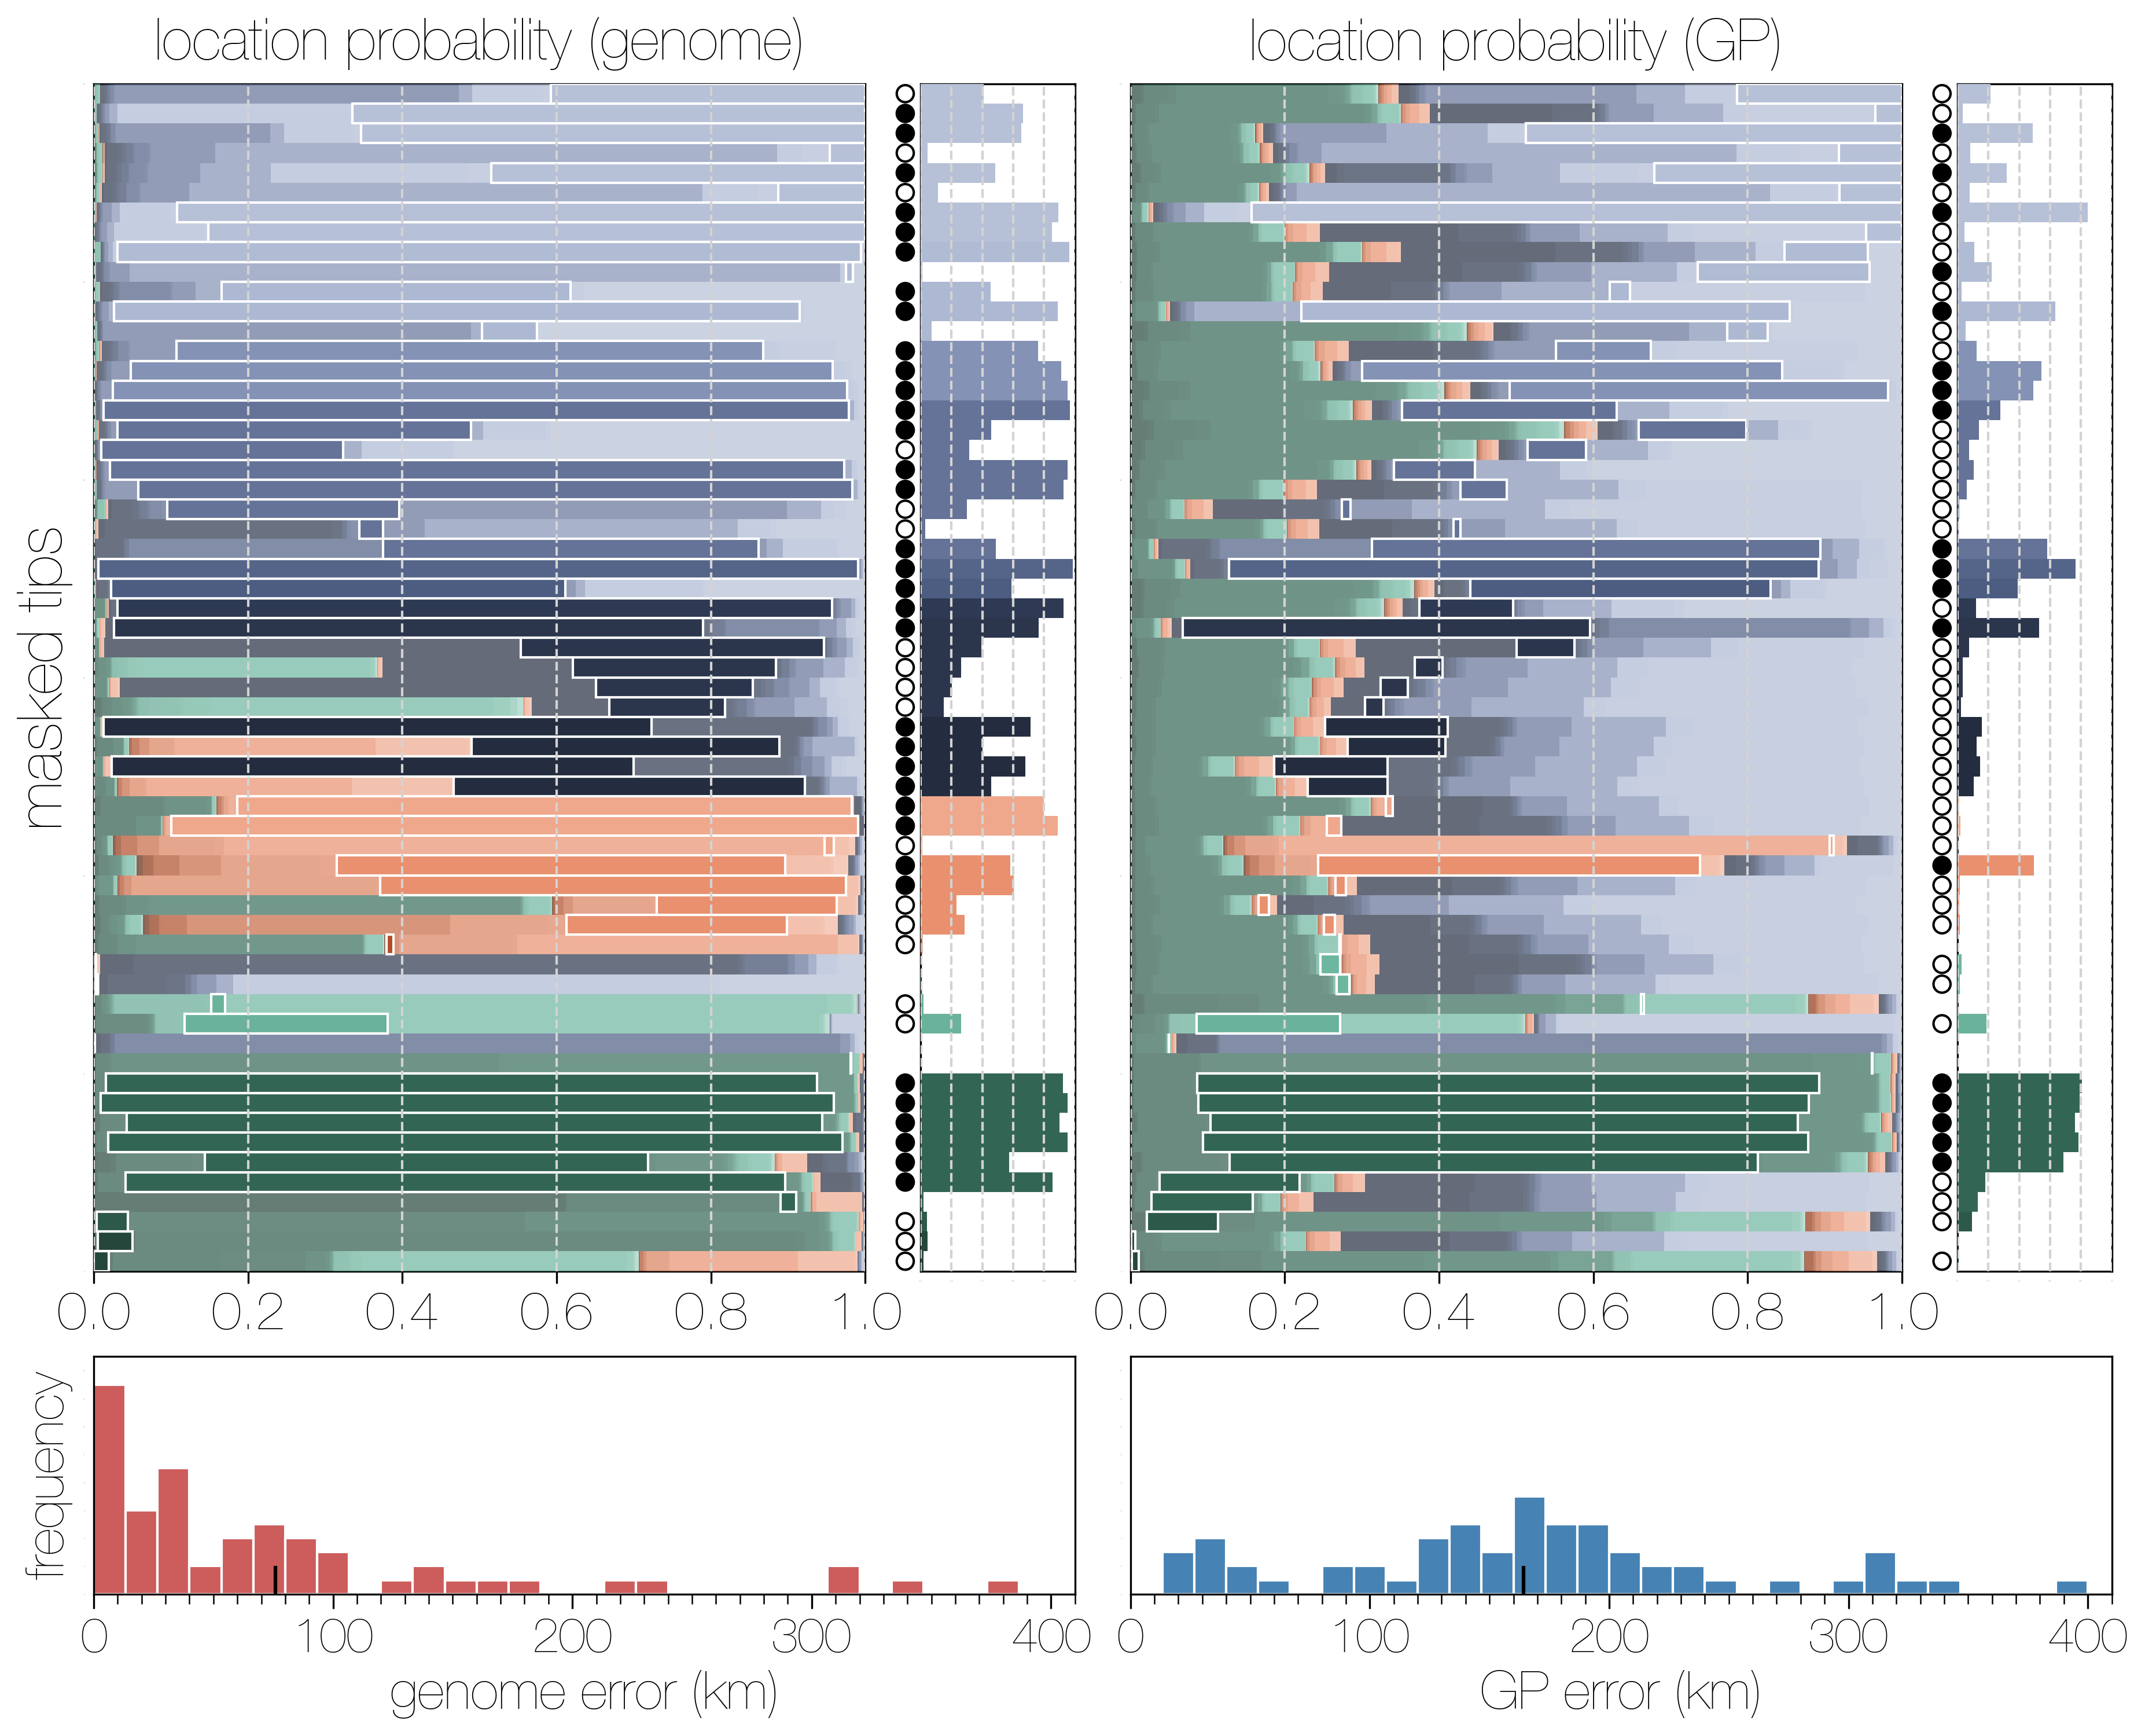
\includegraphics[width=0.75\textwidth]{figures/fig3_locations.png}
	\caption{\textbf{Masked tip location inference from genomes (left) and GP sequences (right).}
  Horizontal bars indicate the posterior distribution of masked tip locations, coloured by country (Sierra Leone in blue, Liberia in red, Guinea in green) and location (lighter colours indicate administrative divisions lying towards west of the country).
  The correct location of each tip is outlined in white, with the smaller plot to the right indicating the posterior probability of the correct location.
  Posterior distribution of probability-weighted distances between population centroids of inferred and correct locations is shown at the bottom with mean indicated by a tick mark.
	}
	\label{locations}
\end{figure}

\begin{figure}[h]
 \centering
  \subfloat{
  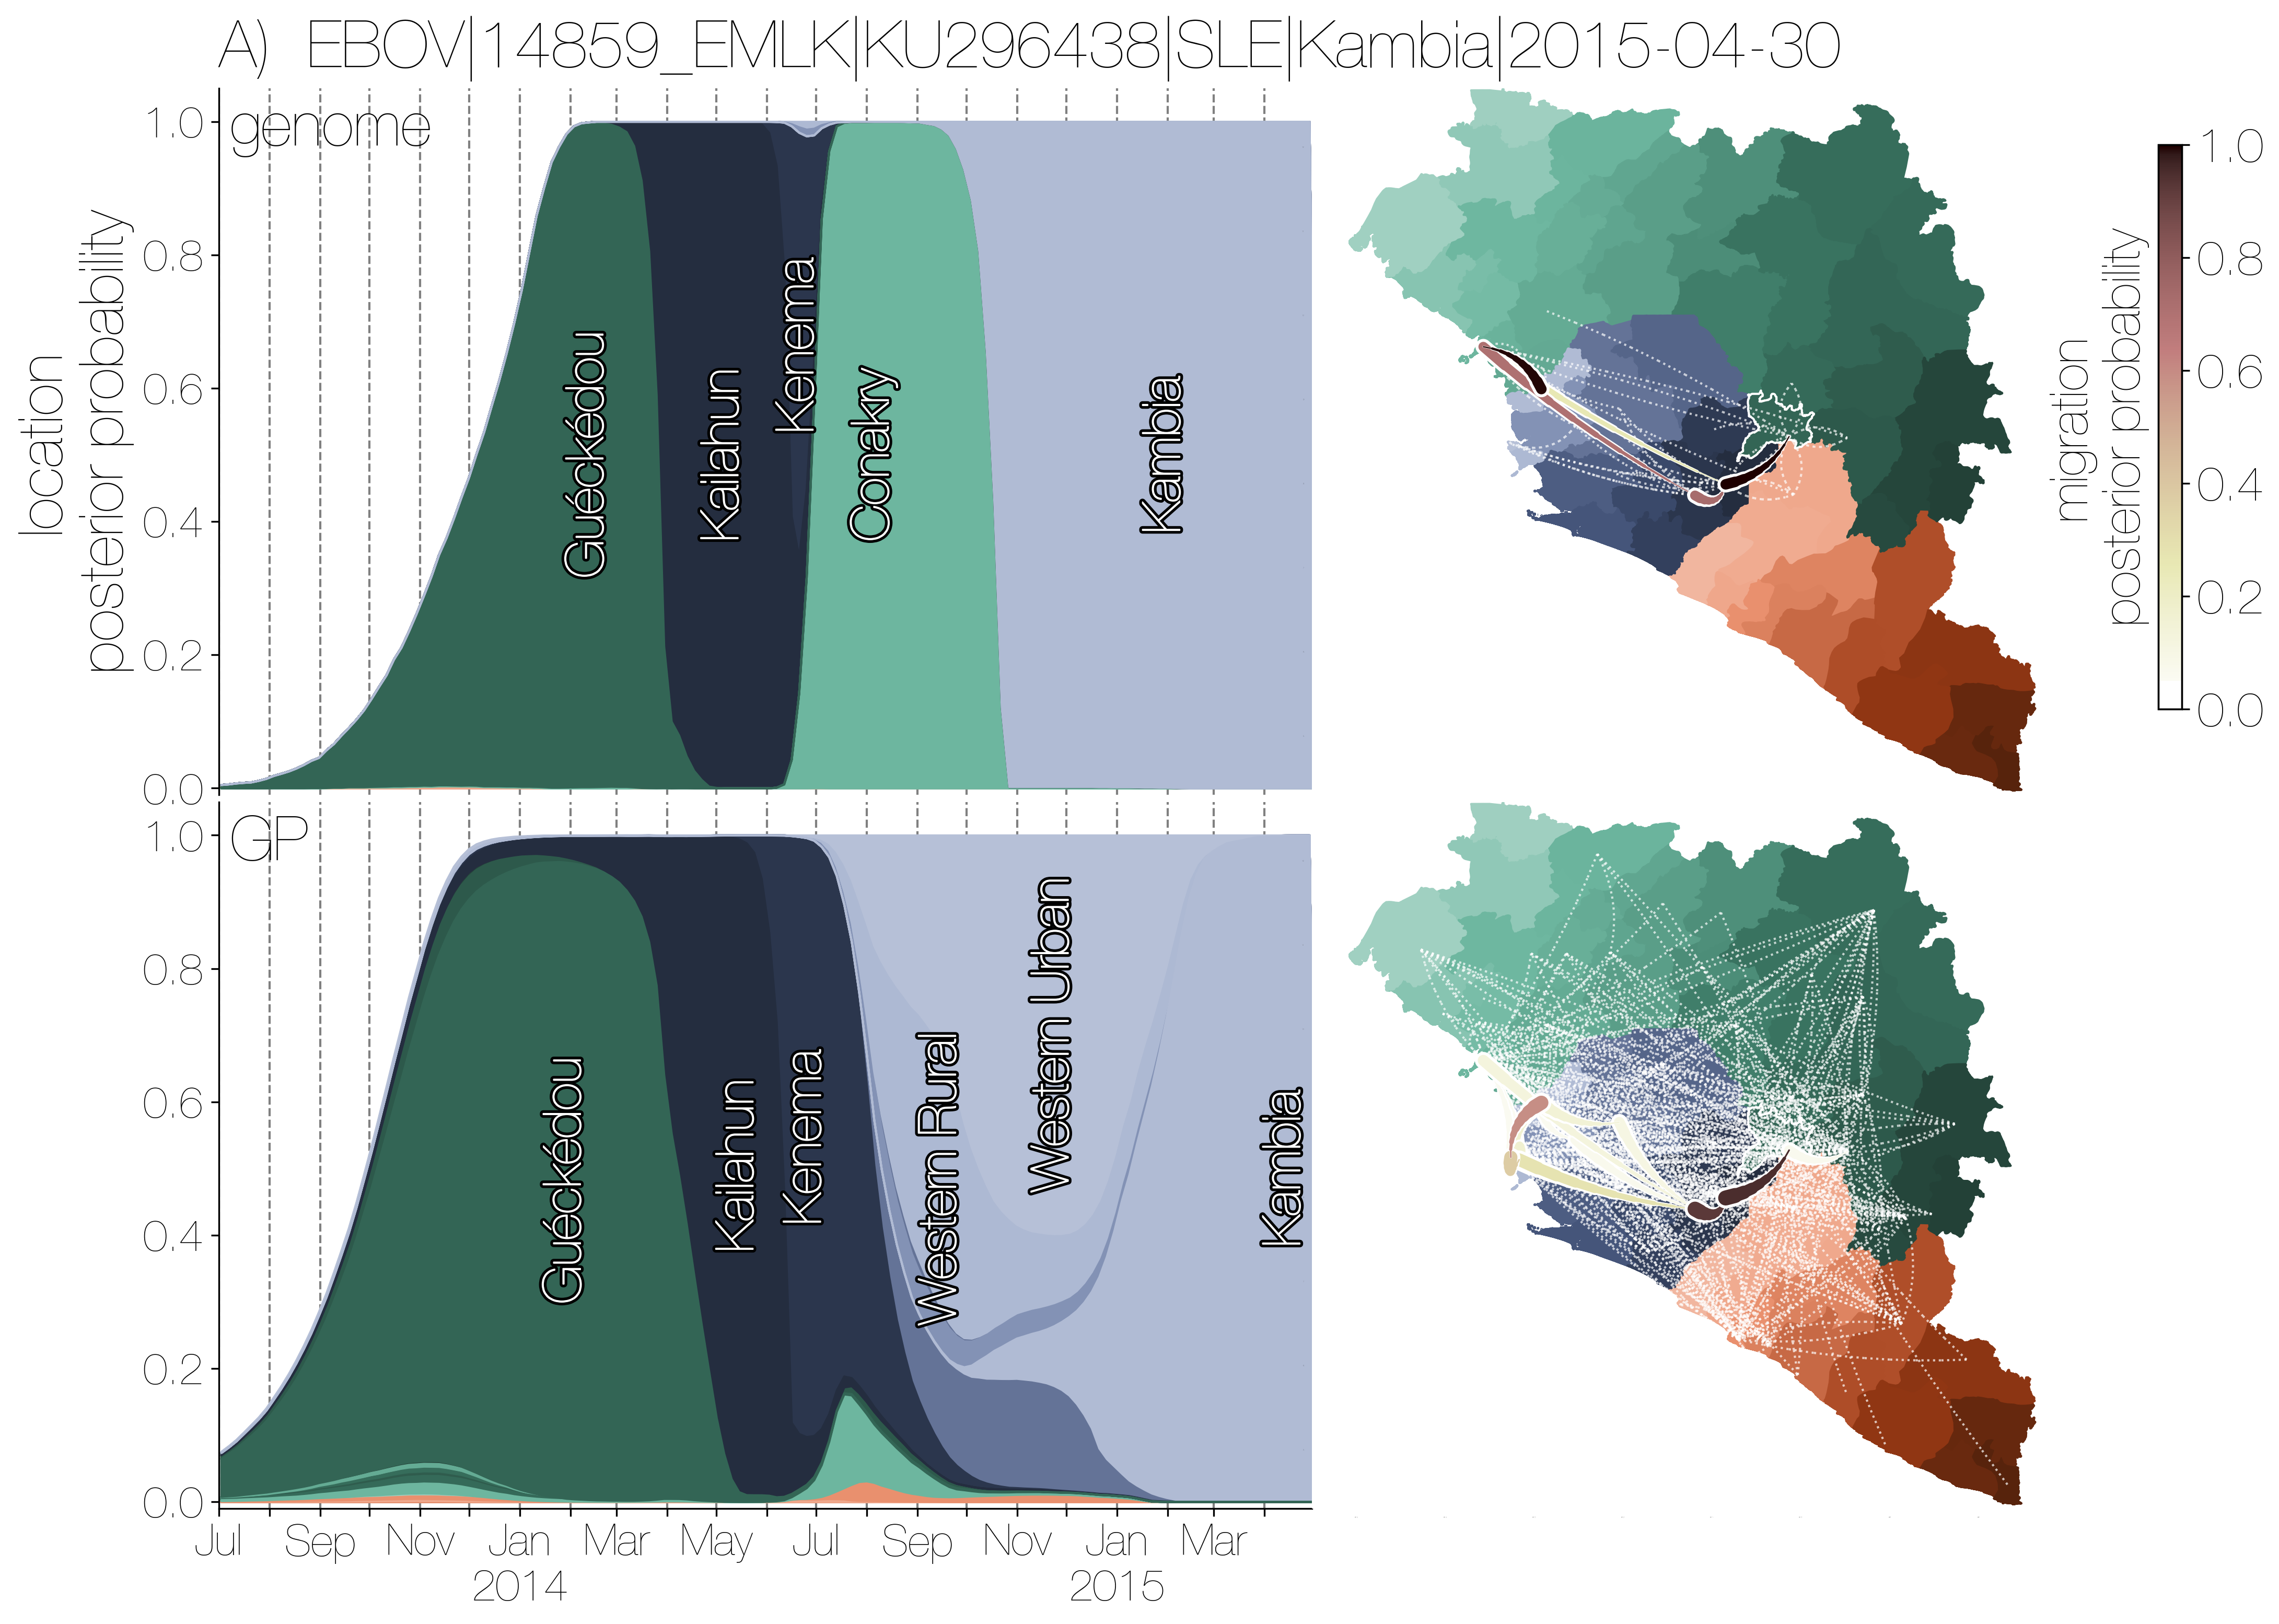
\includegraphics[width=0.45\textwidth]{figures/figXA_histories.png}
  }
  \subfloat{
  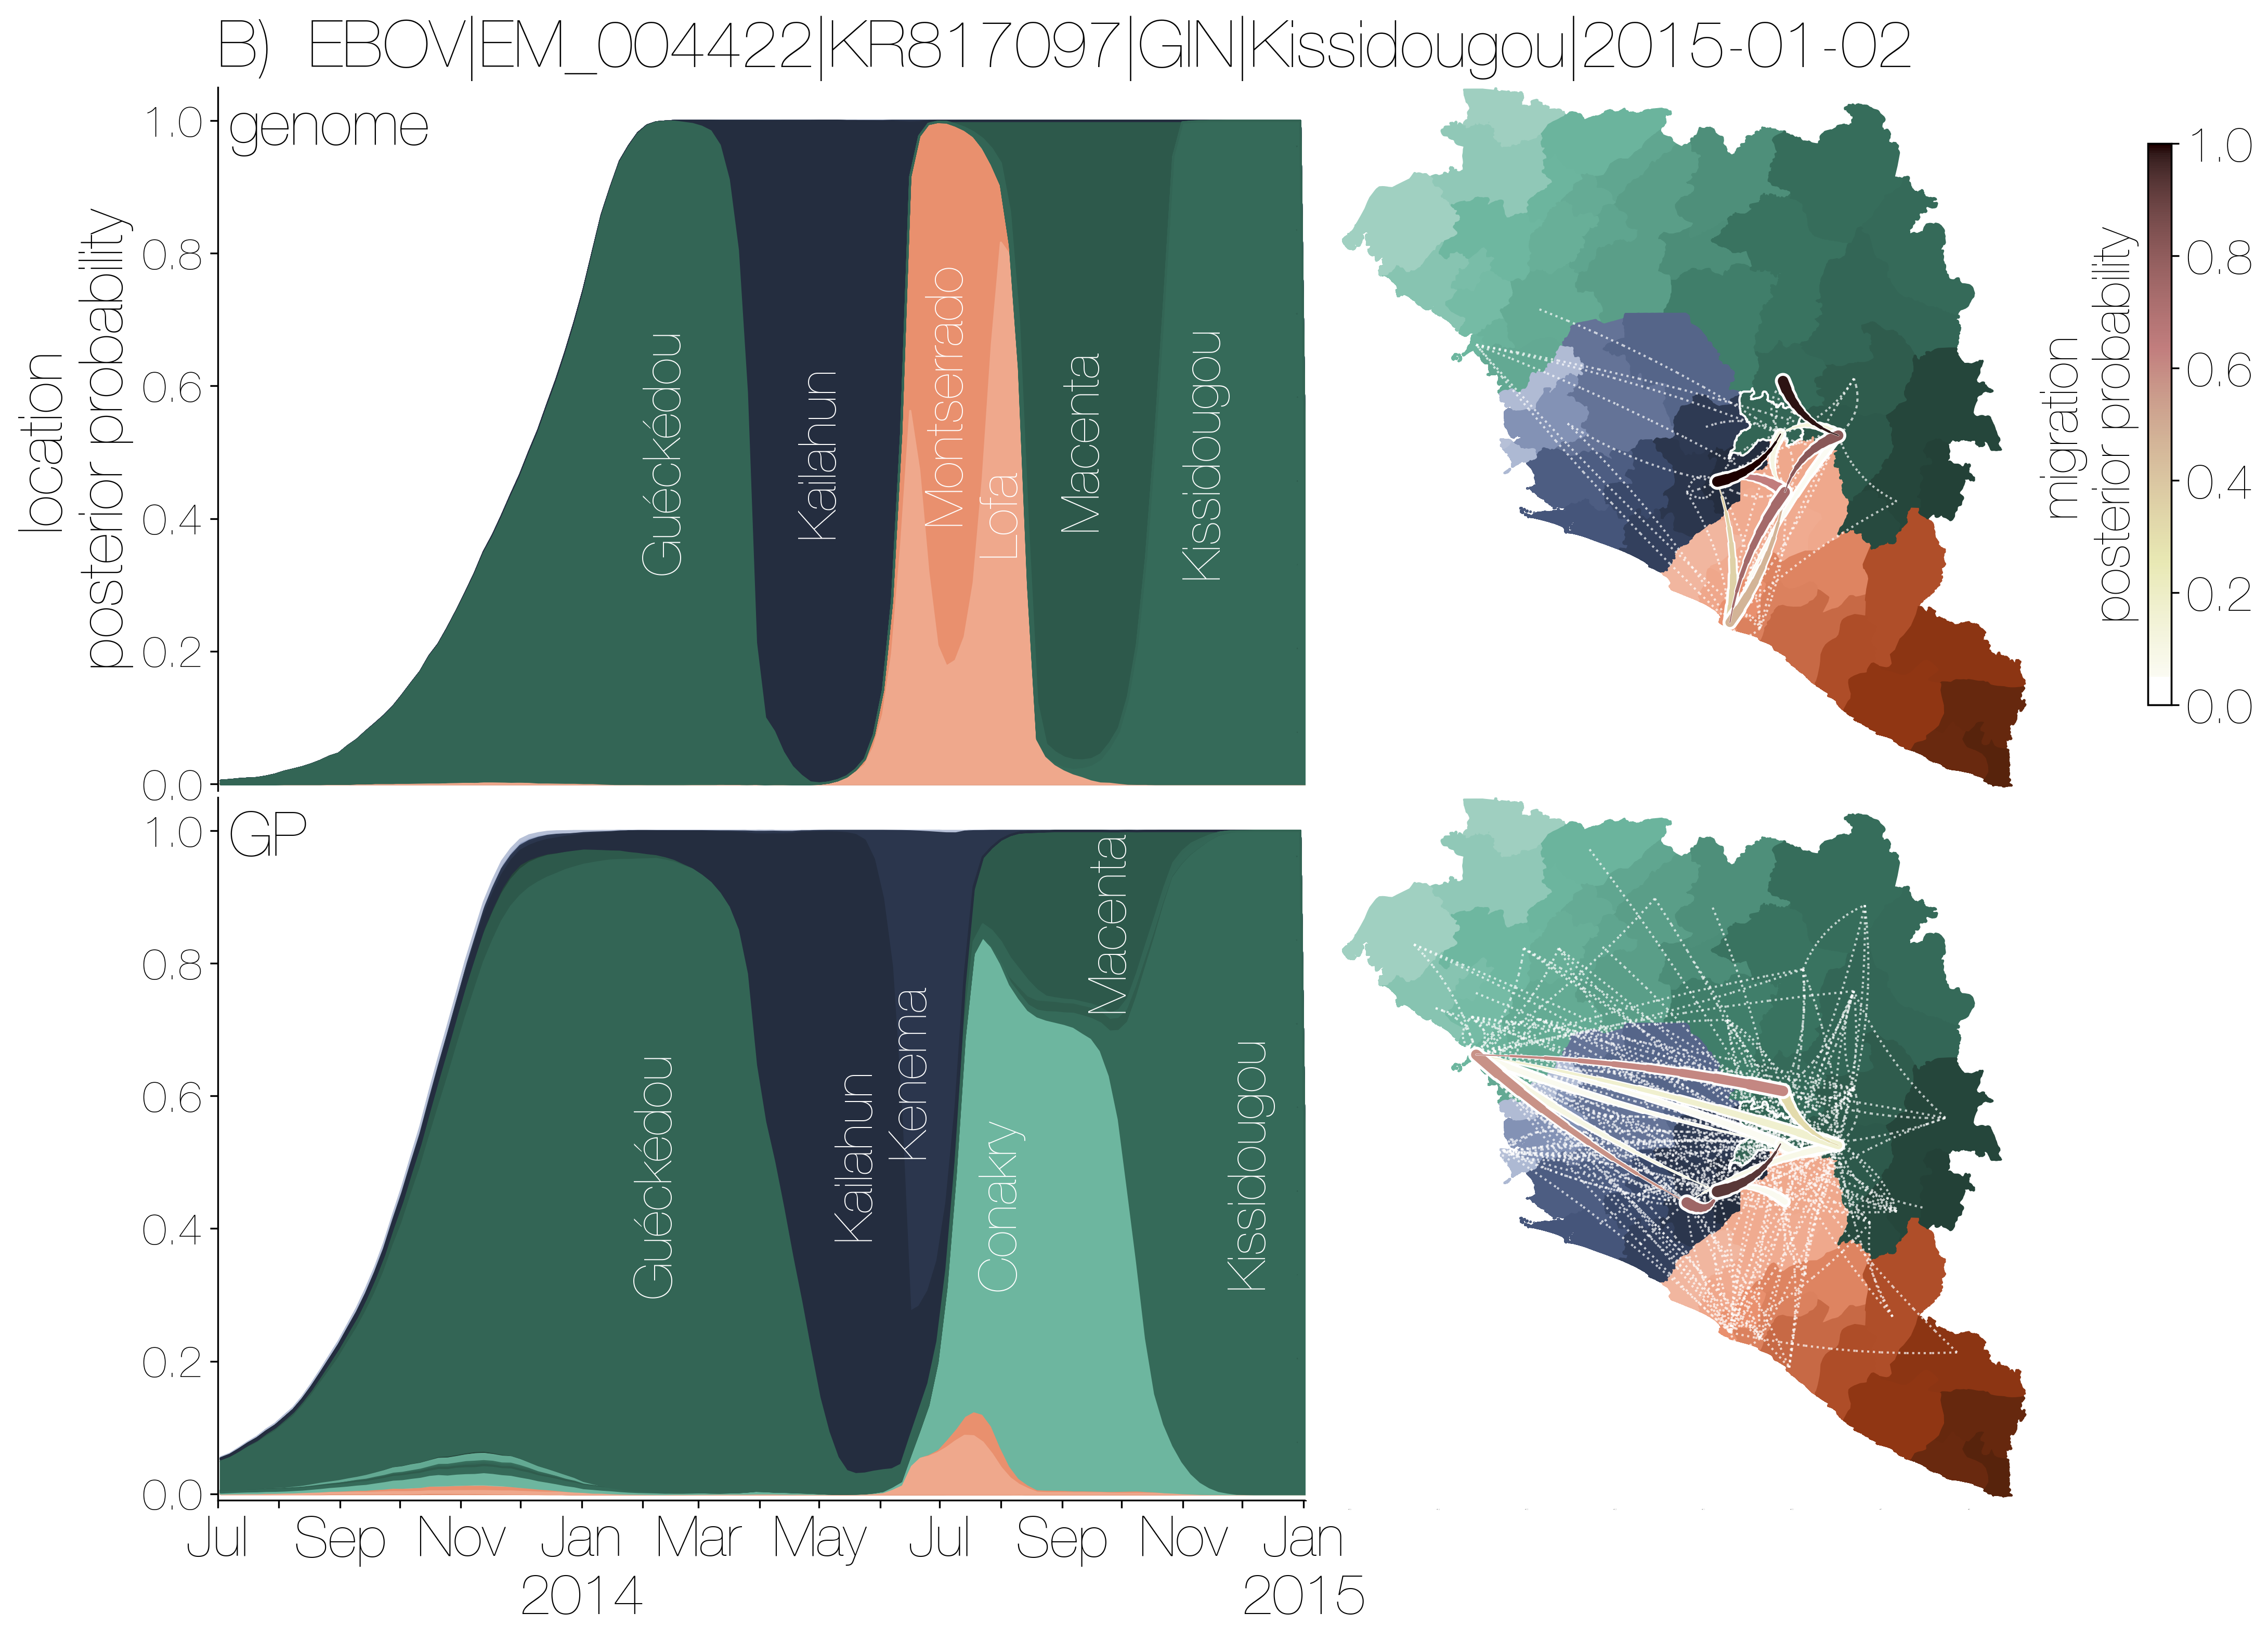
\includegraphics[width=0.45\textwidth]{figures/figXB_histories.png}
  }
  \\
  \subfloat{
  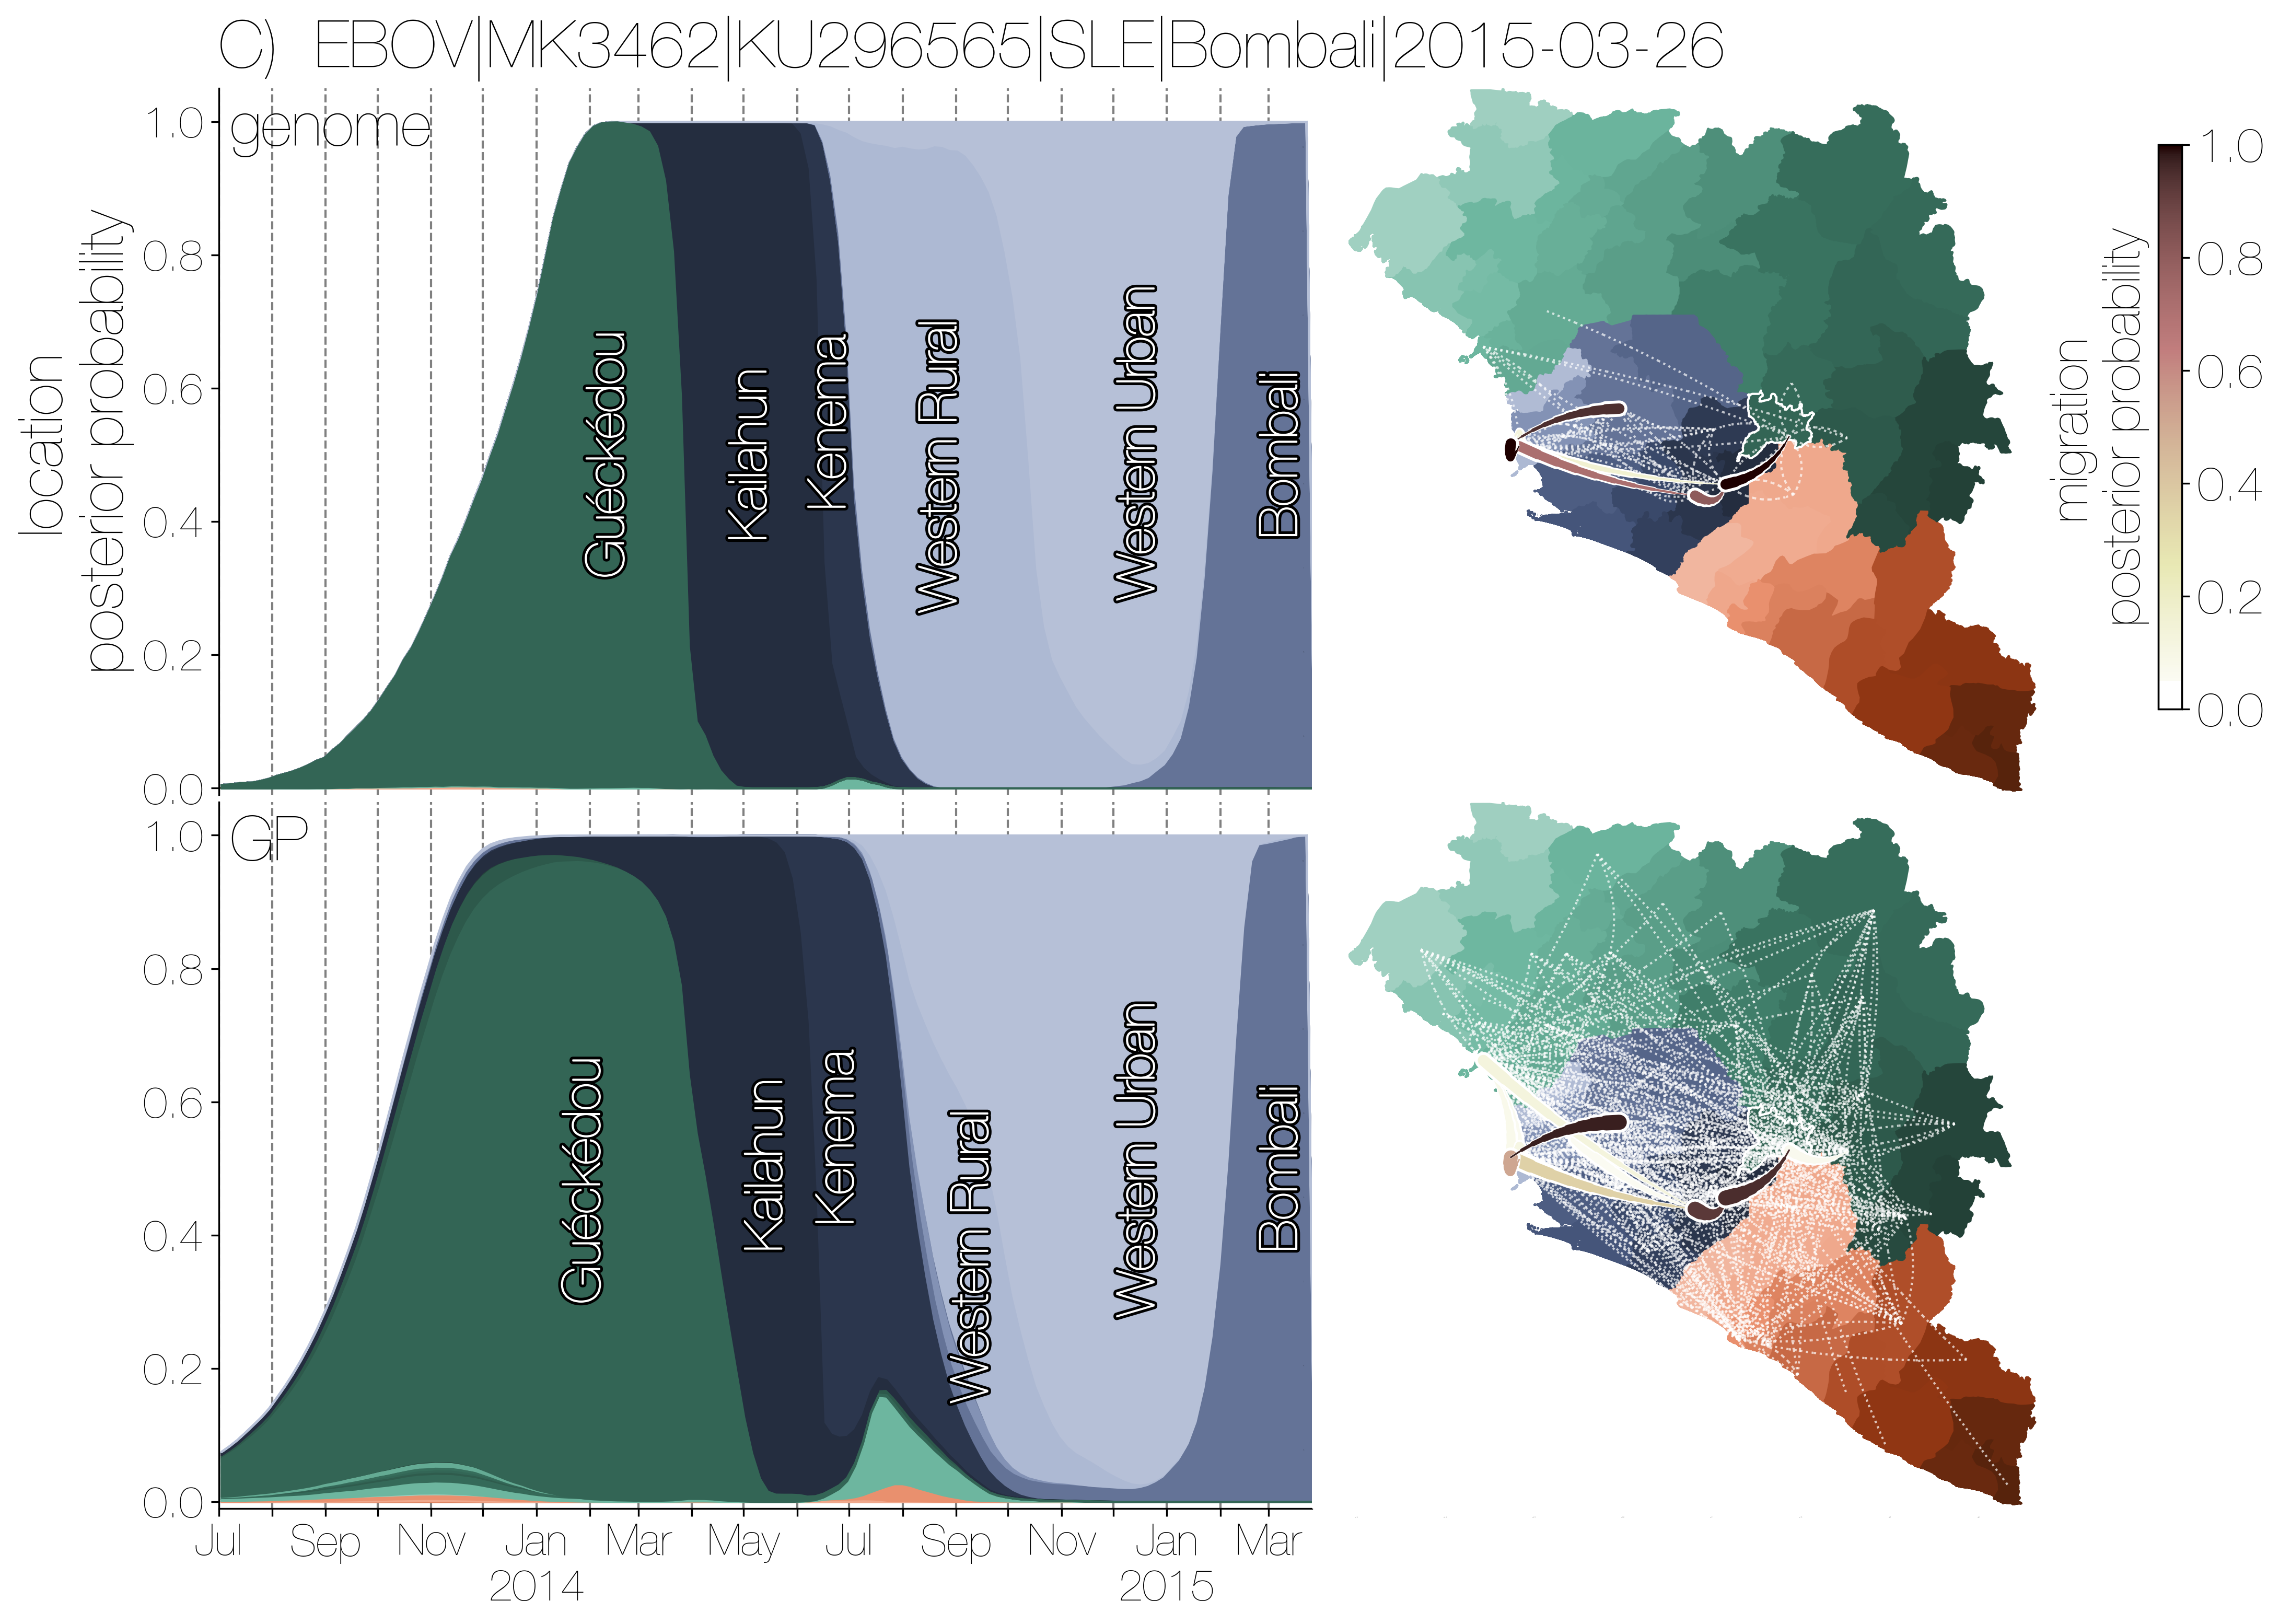
\includegraphics[width=0.45\textwidth]{figures/figXC_histories.png}
  }
  \subfloat{
  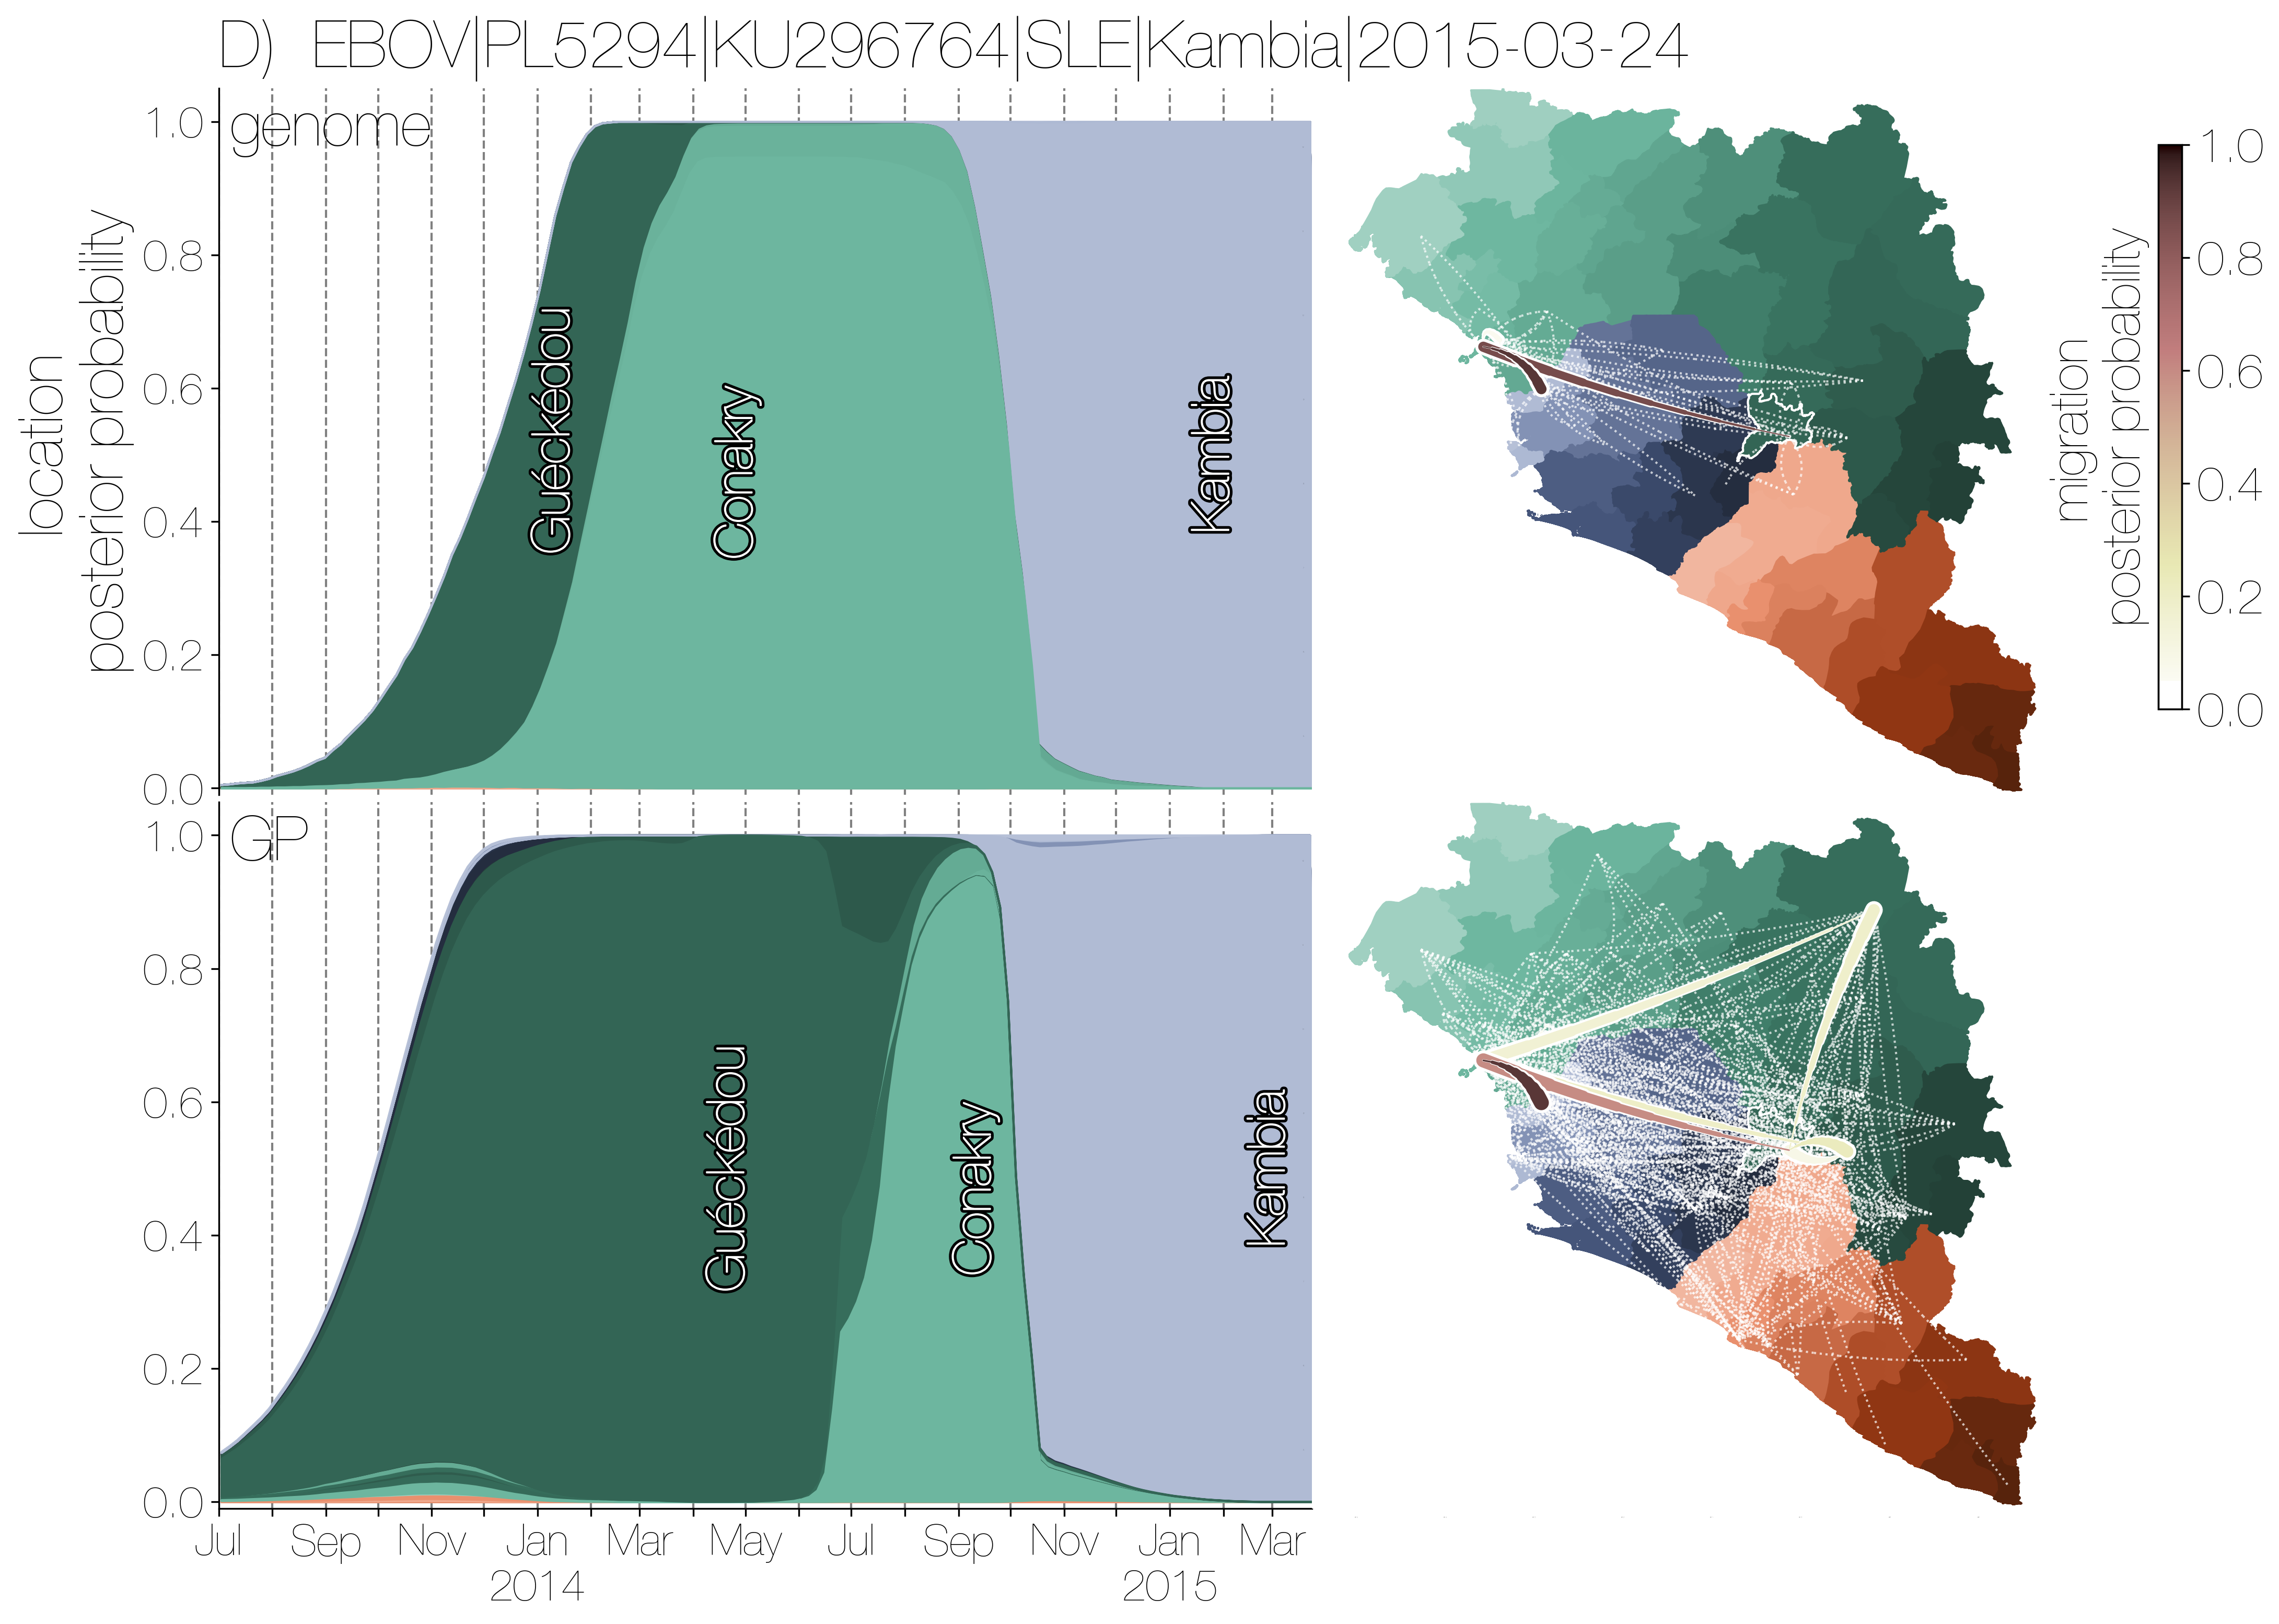
\includegraphics[width=0.45\textwidth]{figures/figXD_histories.png}
  }
  \caption{\textbf{Posterior traces of ancestral locations and posterior migrations for four Ebola virus lineages from genomes (top) and GP sequences (bottom).}
  The inferred ancestral branch location is logged at time points along the path from selected tips to the root of the tree, across the posterior distribution of trees.
  The smoothed trajectories are an indication of where and when a lineage that gave rise to a particular tip existed.
  Maps on the right show migration events that are inferred to have taken place, coloured by their posterior probability, with migrations with <0.05 posterior support are shown as dotted lines.
  All lineages trace back to Gu\'{e}ck\'{e}dou prefecture of Guinea, where the original zoonotic transmission event occurred near the Guinean border with Sierra Leone and Liberia.
  Some lineages are also descended from an early spillover event into Sierra Leone.
  }
	\label{trace}
\end{figure}

\subsubsection*{Loss of power for phylogeographic reconstruction}

Differences between genomic and GP datasets are clear and dramatic when looking at both phylogenies (Fig \ref{trees}) and masked date inference (Fig \ref{dates}), but less pronounced when trying to infer the location of a masked tip (Fig \ref{locations}).
Although locations are correctly inferred more often and with greater support in genomic sequences compared to just the GP gene, there are numerous tips whose locations are not correctly inferred from genome sequences.

This might reflect the nature of these parameters of interest, since phylogenies and date inference ultimately draw information from mutation accumulation via relatively straightforward models of sequence evolution with limited parameter space.
In contrast, migration is a far more complicated and nuanced process without a de facto standard for modelling, though continuous time Markov chain (CTMC) approaches are widely used.
Despite lack of an overwhelmingly obvious contrast between inference of masked location between genomes and GP sequences, cross entropies indicate much better performance with the former, at 6816.772 and 11831.626, respectively.
Similarly, locations are inferred correctly more often with complete genomes than with GP sequences (33 and 18, respectively).
\tbc{Need to more carefully define what you mean by `inferred correctly'. Cross-entropy does this well, otherwise need a cut-off for assignment. Over 50\%?}
Probability-weighted distances to the correct population centroid are also reduced for genomic data, at a posterior mean of 2.870 kilometres compared to 4.315 km for GP sequences.

In addition to assessing how well tip locations can be inferred from genetic information we also looked at how well historical patterns were reconstructed from sequence data.
To accomplish this we looked at the posterior distribution of ancestral locations for four tips with distinct histories.
These are `14859\_EMLK', an infection whose lineage was part of the initial sweep of Ebola virus through Sierra Leone via Kailahun and Kenema districts which ended up in Conakry in Guinea from where it jumped back into Sierra Leone late in the epidemic.
`EM\_004422', which migrated through Kailahun district of Sierra Leone too, but then spread into Liberia from which it spilled back into Guinea via Macenta until being sequenced from a patient in Kissidougou, Guinea.
Similar to other lineages, `MK3462' was part of the sweep through Sierra Leone, though unlike others remained in-country, migrating to the environs of Freetown and then Bombali district where it was sequenced.
`PL5294', unlike others, belonged to a lineage that was not part of the Sierra Leonean sweep and instead part of an unusual and under-sampled lineage endemic to western Guinea, from where it spilled into Sierra Leone's Kambia district late in the epidemic.

The histories of these four tips are, for the most part, reconstructed from both GP sequences and genomes consistently.
However, it is also clear that when using GP sequences location assignment is not as resolute as when genomes are used, and some historically established migration routes are omitted.
Similarly, MCMC with GP sequences explores considerably more low-probability migration paths than genome data.
In the case of `EM\_004422', for example, a series of migrations through distant Conakry are reconstructed with relatively high confidence from GP sequences, compared to shorter distance migrations that run through neighbouring Liberia reconstructed from genomes.

\subsubsection*{Migration models are broadly similar}

\begin{figure}[ht]
 \centering
	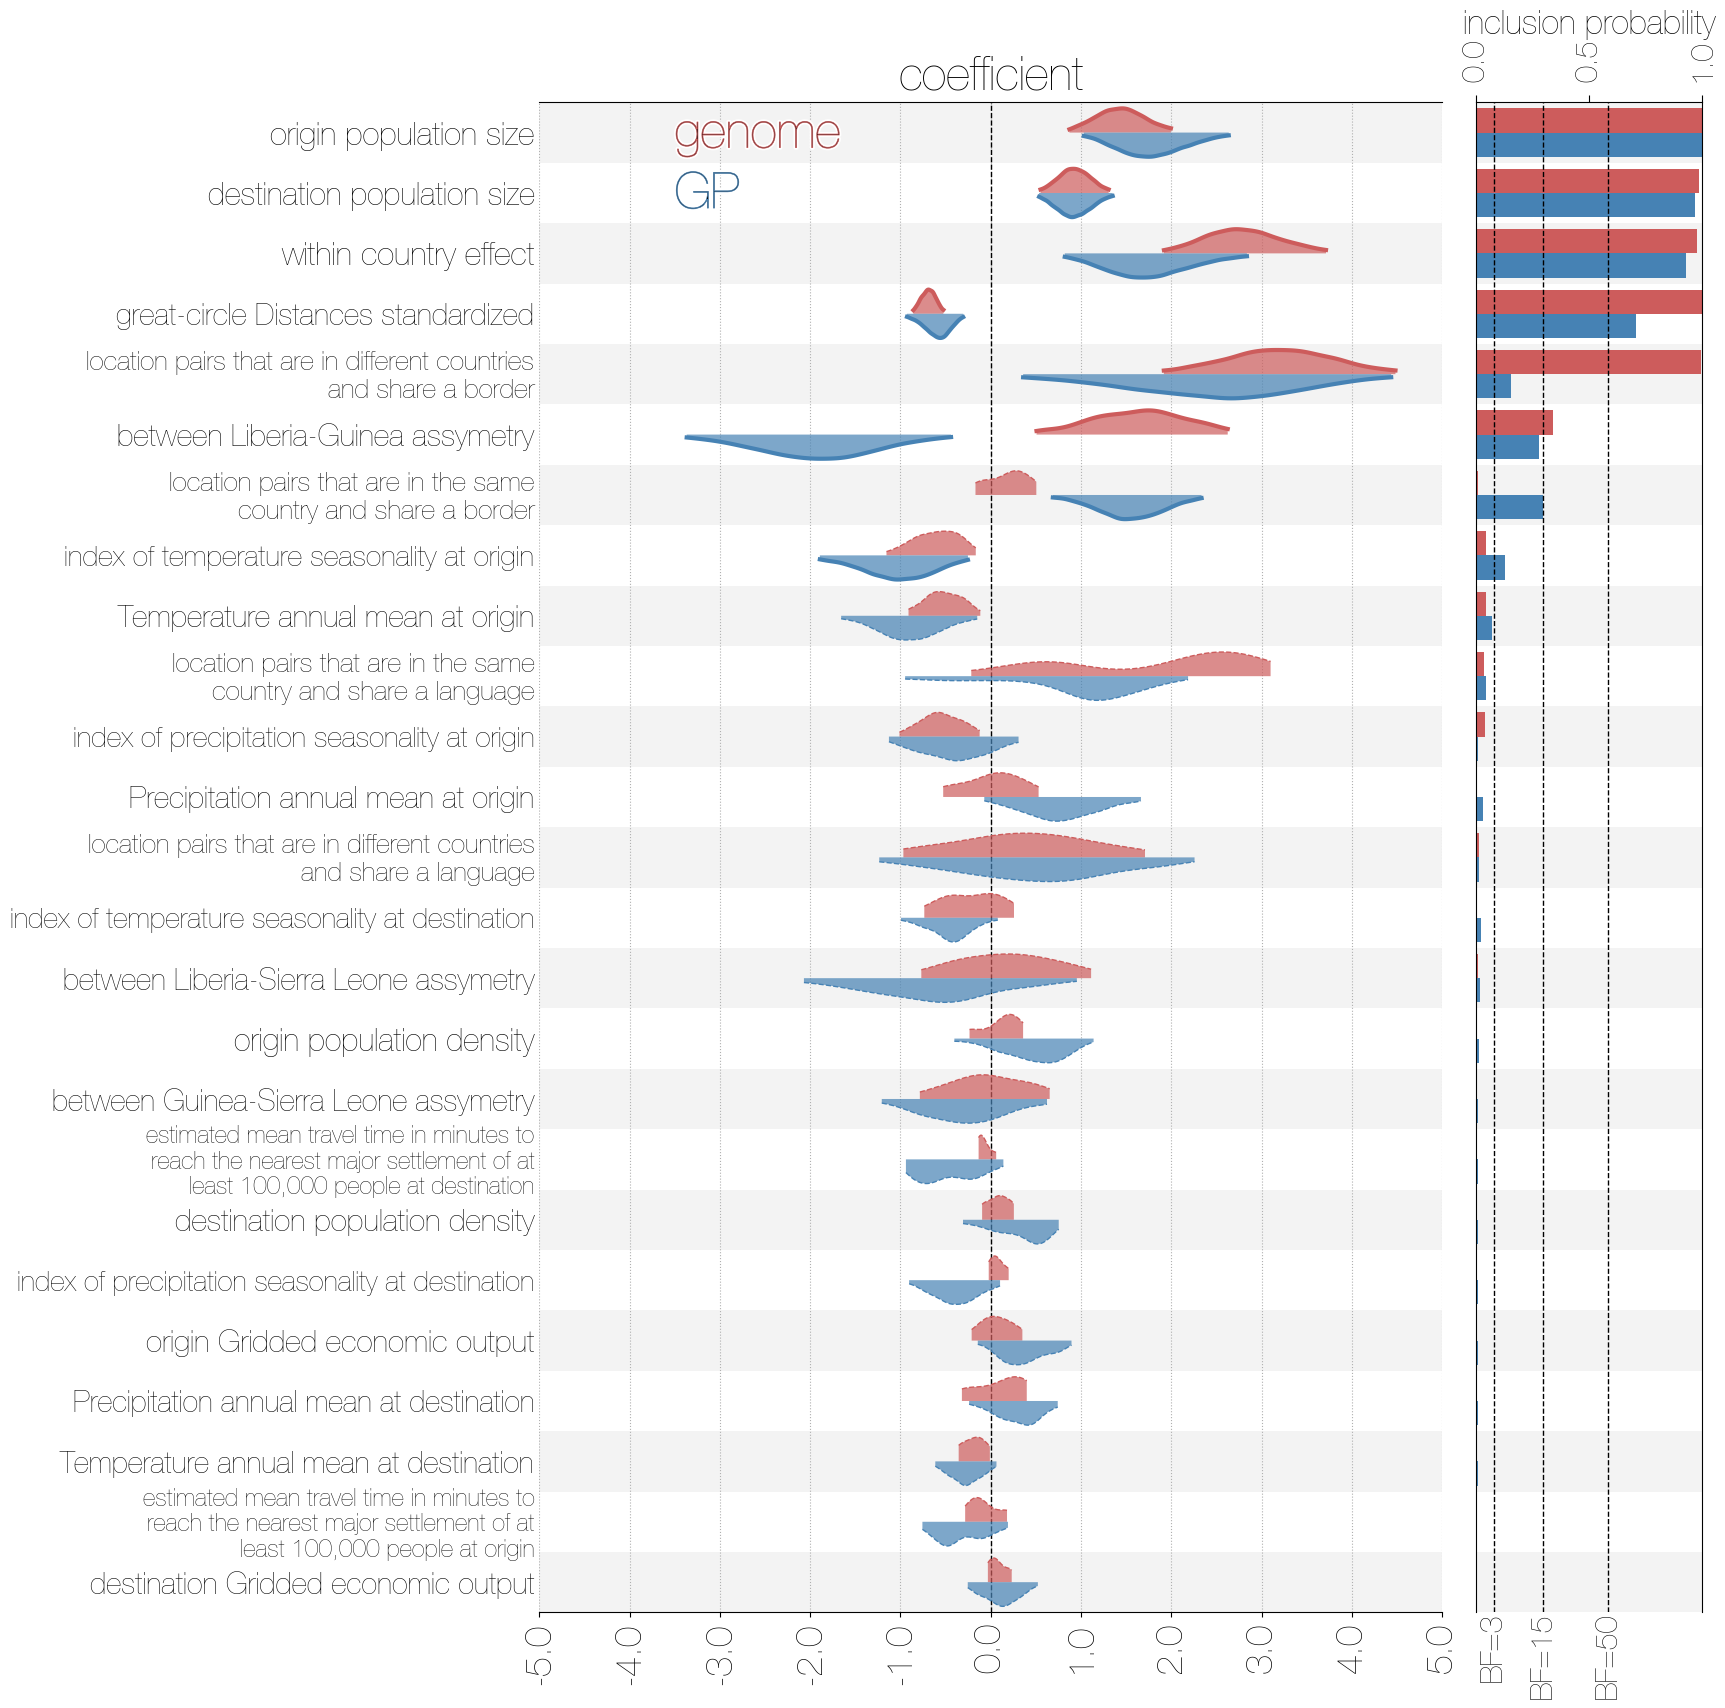
\includegraphics[width=0.75\textwidth]{figures/fig4_glm.png}
	\caption{\textbf{Correlates of migration identified from genomes (red) and GP sequences (blue).}
  Effect size and direction of correlation between predictor matrices and migrations are shown as half violin plots, where the top red kernel density estimates are derived from genomes and bottom blue kernel density estimates are derived from GP sequences, conditioned on the predictor matrix being included in the model.
  Kernel density estimates of coefficients where predictors have <3 Bayes factor support are outlined in dashed lines.
  Posterior inclusion probabilities are shown on the right (red for genomes, blue for GP sequences) with appropriate Bayes factor cutoffs indicated by dashed lines.
	}
	\label{glm}
\end{figure}

Despite markedly reduced information content, the core correlates of migration in the generalised linear model are recovered even with the GP dataset (Fig \ref{glm}).
Population sizes at origin and destination locations, within country effect, and great circle distances are identified as strong predictors of migration with high (>50 Bayes factor, BF), albeit not categorical, support.
Four other migration predictors for the GP dataset have support >5 BF and <15 BF, these are international and national border sharing, Liberia-Guinea asymmetry, and index of temperature seasonality at origin.
Of these Liberia-Guinea asymmetry and international border sharing are also found to be good predictors of migration in genomic data, though confusingly Liberia-Guinea asymmetry has the opposite correlation sign with GP sequence data.
Apart from this deviation, predictors for both genome and GP gene datasets mostly have the same sign and similar effect sizes.

It is likely that reduced phylogenetic information in the GP dataset enables the migration model to explore combinations of predictors that would otherwise be confidently excluded with complete genomes.
This is reflected in total entropy of inclusion probabilities: 1.895 for genome data, and 4.137 for GP sequences.

\subsubsection*{Temporal resolution}

\begin{figure}[h]
 \centering
	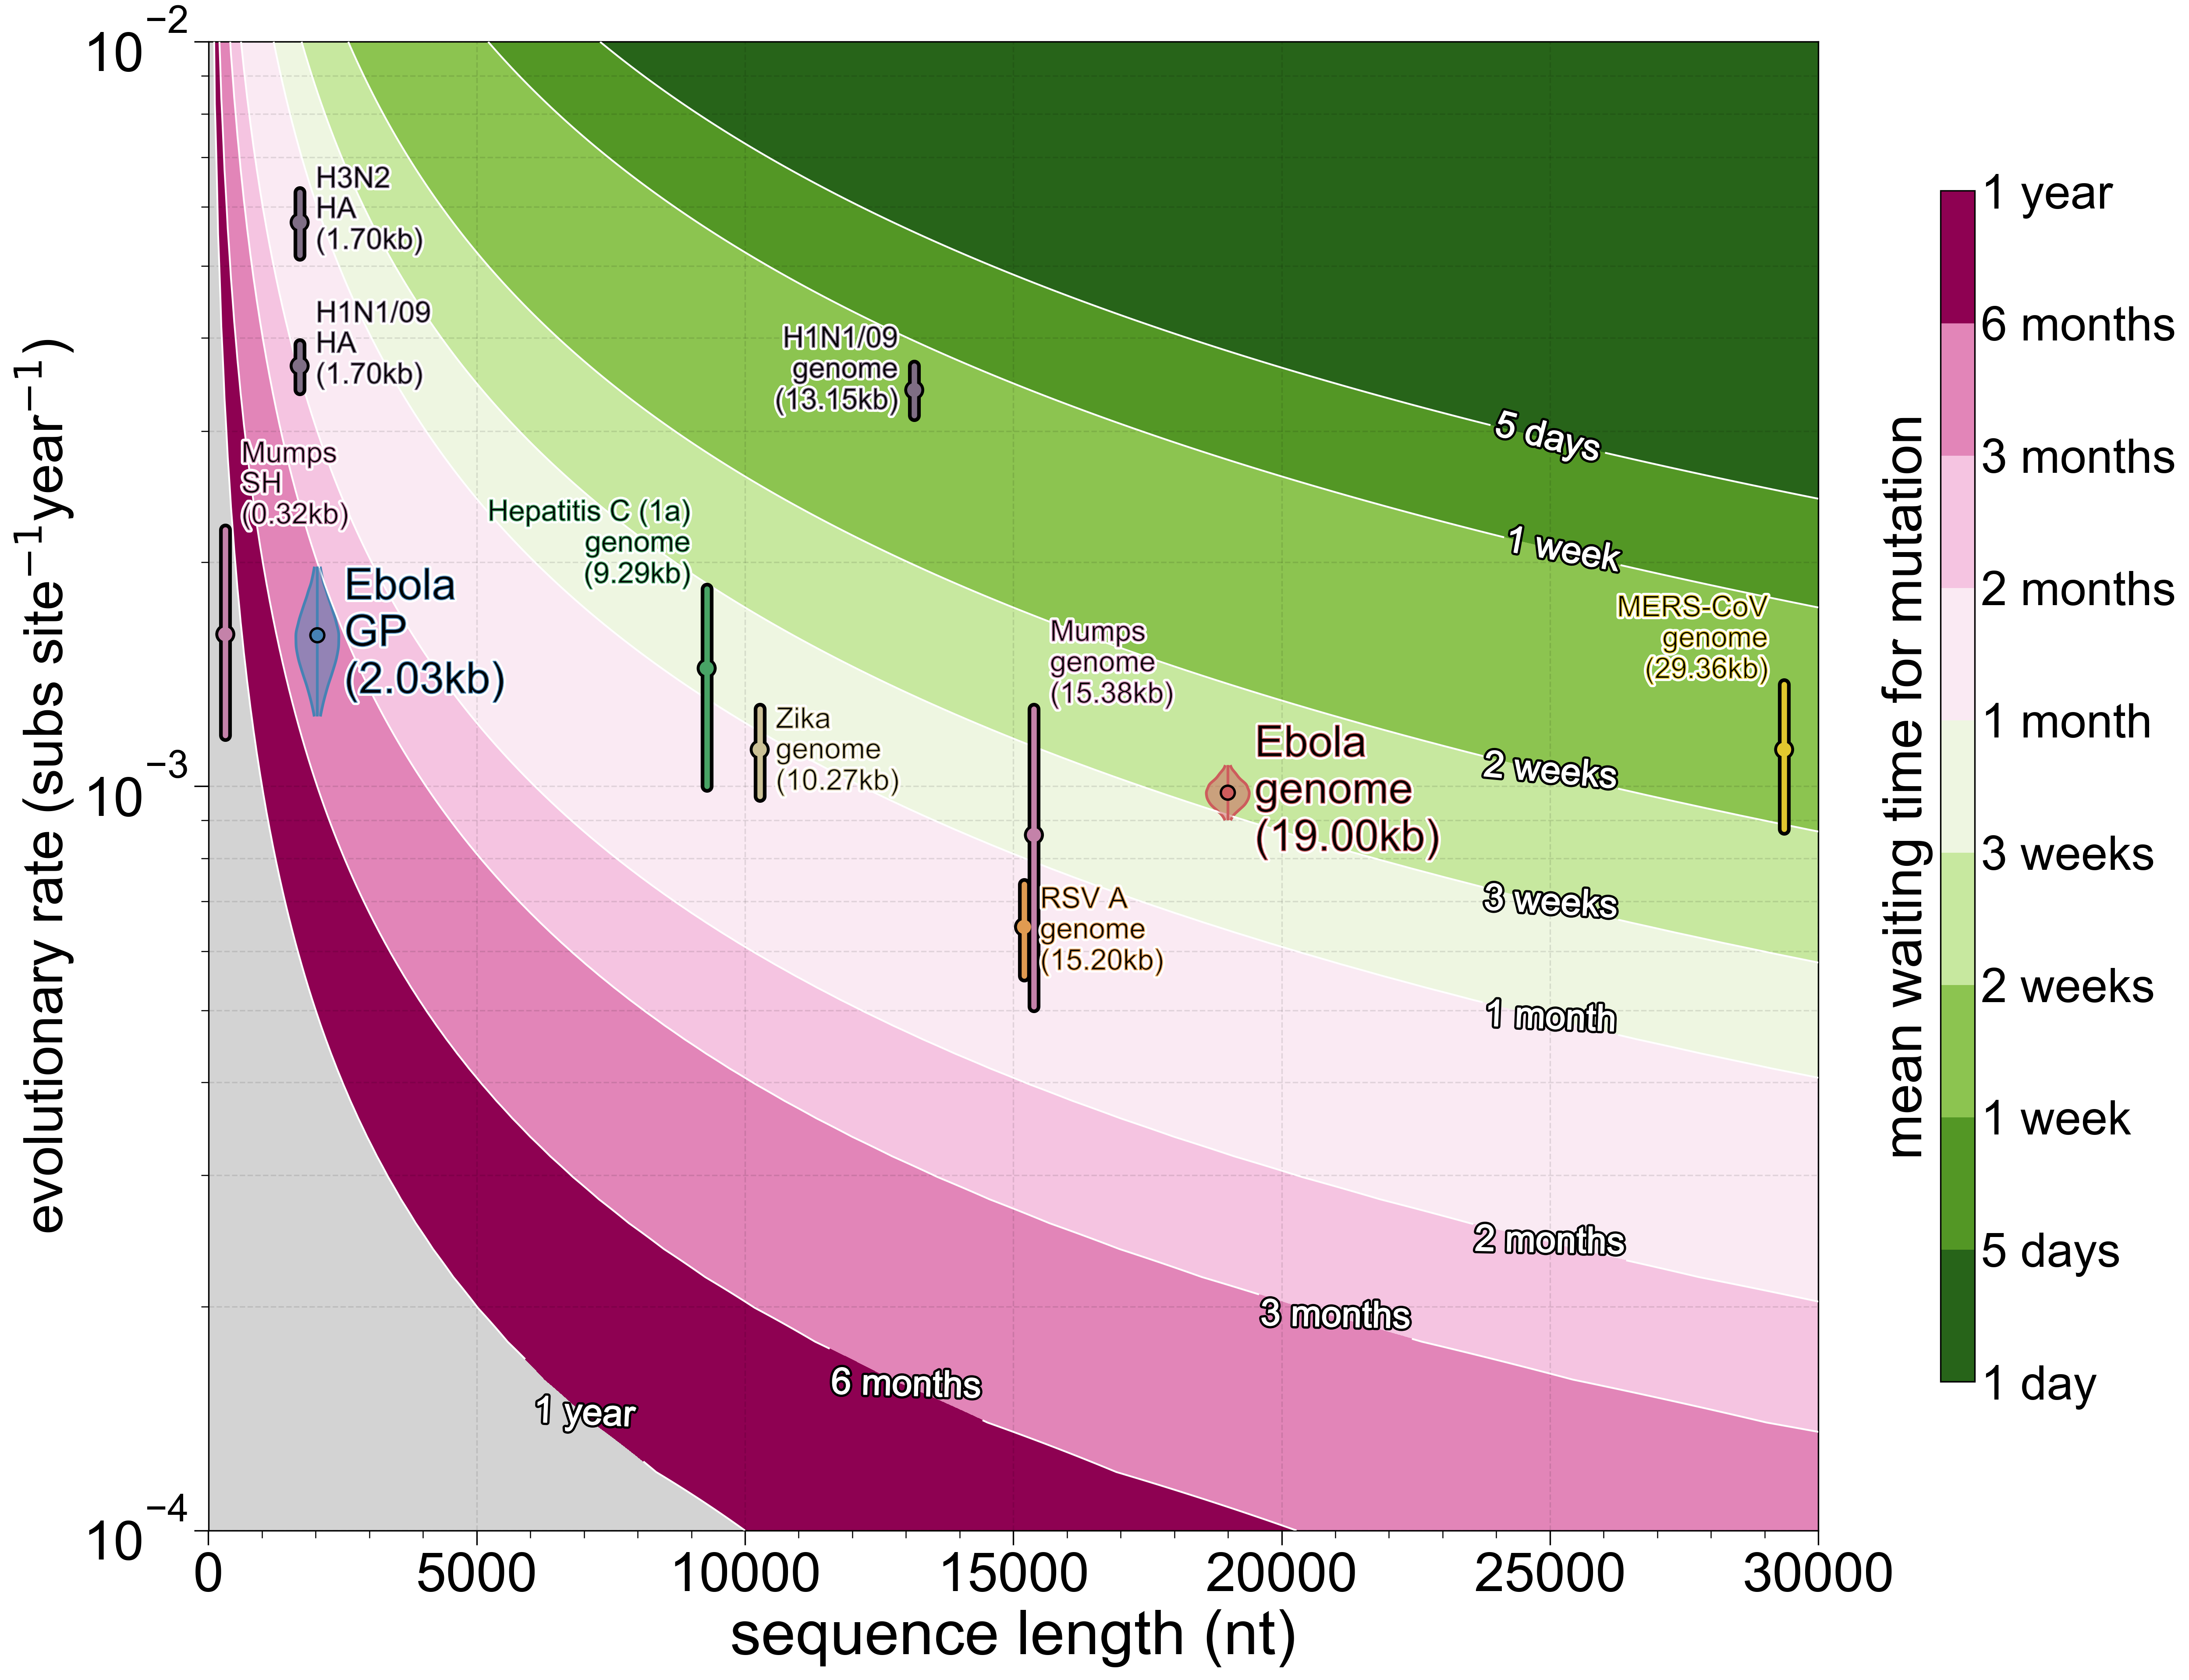
\includegraphics[width=0.75\textwidth]{figures/fig5_contours.png}
	\caption{\textbf{Mean waiting times for a mutation as a function of alignment length and evolutionary rate.}
  Contours correspond to mean waiting times under a given combination of alignment length and evolutionary rate.
  Genomes and barcode genes for a variety of viruses are shown with reported evolutionary rate confidence intervals (vertical lines), including analyses of Ebola virus genomes (red violin) and GP sequences (blue violin) reported here.
  Most genomes occupy parameter space implying temporal resolution of a mutation once every month or so, with mumps virus as an exception.
  Sub-genomic fragments on the other hand are expected to have mean mutation waiting times of more than a month.
	}
	\label{contours}
\end{figure}

As discussed in the introduction, the mean waiting for a mutation is 1/\textit{RL} and depends on the rate at which mutations arise and are sampled by sequencing (evolutionary rate, \textit{R}) and number of sites under observation (alignment length, \textit{L}).
Since 1/\textit{RL} defines a linear relationship between rate \textit{R} and length \textit{L} mean waiting times for mutation can be reduced by an increase in either \textit{R} or \textit{L}.
In order to double temporal resolution one can either double the evolutionary rate \textit{R} or double the alignment length \textit{L}.
The former is generally outside of researchers' control, though genomic regions evolving at a faster rate exist in many pathogens.
How much faster smaller regions are though, will depend on forces of population genetics, such as ability to recombine (strength of Hill-Robertson effect \citep{hill_effect_1966}), as well as positive selection or functional constraints.
It is thus unlikely that significantly higher rates will offset the reduction in resolution caused by focusing on a very small genomic region.
Extending the region that is sequenced, on the other hand, is often trivial outside of resource-limited areas and can dramatically improve temporal resolution.

To help guide researchers we show the relationship between evolutionary rate and alignment length in determining mean waiting times until a mutation is observed in Fig \ref{contours}.
In addition to theoretical expectations we also show where a variety of viral pathogens fall along the two axes - estimated evolutionary rates with uncertainty intervals on the y-axis and alignment length on the x-axis.
Sub-genomic alignments shown in Fig \ref{contours} include the small hydrophobic (SH) gene of mumps virus \citep{cui_evolutionary_2017} and glycoprotein (GP) sequences of Ebola virus analysed in this study, as well as sequences of two human influenza A virues - genome of subtype H1N1/09 \citep{hedge_real-time_2013}, and haemagglutinin sequences of subtypes H1N1/09 \citep{smith_origins_2009} and H3N2 \citep{rambaut_genomic_2008}.
With respect to temporal resolution influenza A virus HAs are expected to acquire a mutation every one to two months on average, compared to around three to six months for Ebola virus GP and over a year for mumps virus SH.
Though all of these sequences are from (-)ssRNA viruses, SH and GP genes are part of a single non-recombining RNA genome \citep{chare_phylogenetic_2003}, whereas HA genes of influenza A viruses are encoded on their own segment which can be unlinked from their genomic background via reassortment.
Because Ebola and mumps virus genomes do not recombine, their polymerases may have been selected for higher fidelity due to Hill-Robertson effect \citep{hill_effect_1966}.

Complete genomes, on the other hand, occupy parameter space that implies that a new mutation occurs on average every month or every few weeks.
This is achieved through having more sites rather than substantial differences in evolutionary rates, which differ only marginally with respect to subgenomic fragments.
Despite this, no virus is expected to acquire mutations faster than about once per week on average, and the two genomes with highest predicted temporal resolution - MERS-CoV and H1N1/09 - are difficult to analyse due to recombination and reassortment, respectively.
The inverse relationship between observed evolutionary rate and sequence length is similar, but not the same as the relationship between virus genome sizes and mutation rates, where high mutation rates and large genome sizes lead to substantial deleterious mutation load \citep{gago_extremely_2009}.
This upper limit on mutation waiting times set by optimal evolutionary rates is what we refer to as the temporal horizon - population processes with inverse of rate (\textit{i.e.} waiting time) less than the rate at which a pathogen acquires mutations will not be captured with high fidelity by currently existing methods.
The exact relationship between mutation waiting times and rates of processes will, of course, be complicated by the presence of co-circulating lineages, site-wise rate heterogeneity, and choice of model for population processes of interest.

\section*{Conclusions}
\subsubsection*{Theoretical considerations}
For studies focused on temporal dynamics of pathogens over shorter periods of time the waiting time for a mutation should ideally be smaller than the inverse of the rate at which a process of interest occurs.
Serial interval is often of most interest usually and has been addressed previously \citep{campbell_when_2018}, but migration or cross-species transmission rates could also exceed the critical temporal resolution threshold if sequences are assigned to compartments that are too small.
It is likely that this resolution limit will be improved greatly in the future by including additional information, either some aspects of a known transmission tree or, more likely, pathogen variation at the within-individual level, where variant sharing between two or more individuals is evidence of their linkage in a transmission cluster.
Much like evolutionary rates, these methods might encounter biological limits outside of researchers' control, however.

In addition to emphasising the need to sequence complete pathogen genomes, we also hope that our study imparts the interpretation of pathogen evolutionary rates as primarily a parameter indicating temporal resolution of sequence data.
It has been argued that low within-outbreak divergence in Ebola virus GP during the outbreak in Kikwit, DRC in 1995 was evidence of ``genetic stability'' \citep{rodriguez_persistence_1999}.
Conversely, many studies misconstrued the high evolutionary rate at the whole genome level observed within the West African Ebola virus epidemic as evidence of rapid adaptation of the virus to humans (addressed by \cite{holmes_evolution_2016,rambaut_comment_2016}), despite no such statement in the original study \citep{gire_genomic_2014}.
In the case of the former not enough time had passed for mutations to accumulate to any significant degree within the relatively small GP gene, in the latter complete genomes were sequenced from nearly the entire transmission chain, capturing most of the mildly deleterious variants circulating at the time.
Inaccurate interpretations of evolutionary rate, not accounting for the passage of time and alignment length were misinterpreted as evolutionary forces, rather than limitations of data at hand.

There is an additional Bayesian phylogenetic argument to be made in favour of using complete genomes.
Molecular clock phylogenetics often relies on Markov chain Monte Carlo sampling to approximate the posterior distribution of phylogenetic trees \citep{yang_bayesian_1997}.
Sequences which fall into polytomies in substitution phylogenies (\textit{i.e.} well-defined common ancestry, but no indication of exact branching order) are particularly problematic, since plausible temporal phylogenies can be reconstructed in the absence of mutations.
The branching order of such clades in time trees will be determined via tree and molecular clock rate priors, since no information about branching order can be recovered from the sequences themselves.
There are over 34 million possible rooted trees for a set of 10 sequences, some of which will be visited less often during MCMC if sequences are collected over time and the product of effective population size and generation time ($N_{e}\tau$) are low.
Nonetheless, MCMC is inefficient at sampling any individual topology for identical sequences \citep{whidden_quantifying_2015}, since the space of possible trees is expanded without adding additional information.

\subsubsection*{Practical considerations}
As well as temporal resolution concerns raised previously there are practical issues to consider when sequencing pathogens.
Although many pathogens have established ``barcode'' genes or regions \citep{towner_rapid_2004}, some do not.
This can easily lead to different groups sequencing different pathogen genes by chance or choice \citep{georges-courbot_isolation_1997,leroy_fruit_2005,rouquet_wild_2005}, which is not necessarily a problem when sufficient complete genomes are available to bridge information between disparate regions and appropriate methods of analysis are chosen \citep{dudas_phylogenetic_2014}.
Thus sequencing complete pathogen genomes, in addition to providing the best possible resolution temporally in terms of mutation content, also ends up aiding in standardising data between studies.
Pathogen genomes represent a complete unit of data, in the sense that it is impossible to sequence more than the full genome, that disparate groups can agree to target for sequencing.

It is also worth considering that the lifetime of sequence data extend beyond publication.
Most scientific studies are designed with specific questions in mind that guide how data are collected.
Combining data across studies with different goals can therefore present a challenge.
Sequence data, on the other hand, become difficult to combine at high levels of divergence when multiple sequence alignment algorithms lose the ability to establish homology between sequences.
Since divergence levels are generally low within outbreaks (with exceptions \citep{andersen_clinical_2015}), sequence data are often trivial to combine.
More than that, including sequence data from previous studies can reciprocally contextualise both older and newer sequences (\textit{e.g.} \cite{mena_origins_2016}).
What remains problematic is determining and standardising additional data pertaining to the sequences themselves (``metadata'') in a way that makes sequence data easy to use by other groups.
Whilst date and location of collection are widely reported and often of most interest, non-standard encodings of both are seen on public databases.

\subsubsection*{Stating the obvious}
It is not at all surprising that reducing the number of alignment columns by 10\% from nearly 19,000 nucleotides that comprise the entire Ebola virus genome down to around 2,000 nt of the GP gene can result in loss of information, even if the shorter region evolves at a faster rate.
Here, we have quantified this loss of information via several methods: raw phylogenetic resolution (Fig \ref{trees}), molecular clock signal (Fig \ref{dates}), and phylogeographic models (Figs \ref{locations}, \ref{trace}, and \ref{glm}).
In most cases biological aspects of the data, such as precise branching order and molecular clock resolution, suffer the most loss of resolution, whereas modelling of non-biological aspects of the data, such as migration, tend to be more robust.
This might be caused by the temporal structure of the sequence data \citep{boskova_influence_2018}, since Ebola virus in West Africa was highly mobile and exhibited limited local circulation.
This might explain why in many cases when comparing analysis results between genome and GP datasets statistical power remains disproportionately high, despite retaining only ~10\% of available sites and mutations.
On a similar note, case numbers alone have been used to recover a gravity-like model for the spread of Ebola virus in West Africa \citep{kramer_spatial_2016}.
The overall conclusion from our study, as well as others \citep{wohl_co-circulating_2018}, is that sequencing short genomic regions, instead of whole genomes is an ill-advised practice for investigating infectious disease outbreaks in any appreciable detail across relatively short timescales.

\section*{Methods}
\subsubsection*{Sequence data}
A publicly available dataset of 1610 Ebola virus genomes sequenced by various groups \citep{baize_emergence_2014,gire_genomic_2014,park_ebola_2015,carroll_temporal_2015,kugelman_monitoring_2015,ladner_evolution_2015,simon-loriere_distinct_2015,tong_genetic_2015,arias_rapid_2016,smits_genotypic_2015,quick_rapid_2015} and systematised in \cite{dudas_virus_2017} was filtered to remove sequences where over 1\% of the genome sequence was ambiguous or the precise location down to administrative division was not available, leaving 943 genomes.
A set of 600 viral genomes were randomly sampled from the filtered dataset of 943 high quality genomes.
Of the 600 genomes that were chosen for analysis 10\% (60 genomes) were chosen for masking, where for all subsequent analyses both the date and location were considered as unknown and inferred as latent variables.
Date inference was constrained to the period 2013 December 01 to 2015 December 01, corresponding roughly to the presumed beginning of the epidemic in late 2013 and end in autumn of 2015.
Another dataset was generated by extracting the glycoprotein GP coding sequence (with padding inserted into the polymerase slippage site) from the complete genomes dataset, resulting in an alignment 2031 nucleotides long.

\subsubsection*{Bayesian analyses}
Both GP and genome datasets were analysed in BEAST v1.8.10 \citep{suchard_bayesian_2018} under the GLM model described previously \citep{faria_simultaneously_2013,lemey_unifying_2014,dudas_virus_2017} to infer the migration model, as well directly on the continuous time Markov chain migration matrix with Bayesian stochastic search and variable selection (BSSVS) procedure \citep{lemey_bayesian_2009}.
Sites in both GP and genome alignments were partitioned into codon positions 1, 2, and 3, with the genome analysis also including a partition comprised of non-coding intergenic regions.
Each partition was assigned an independent HKY+$\Gamma_{4}$ \citep{hky_1985,yang_1994} substitution model.
A relaxed molecular clock with an uninformative prior on the mean \citep{ferreira_bayesian_nodate} of the log-normal distribution was used as the clock model \citep{drummond_2006}.
A flexible skygrid tree prior \citep{gill_2013} was used to infer estimates of effective population size across 100 evenly spaced points in time starting 1.5 years prior to the collection of the most recent sequence to the date of the most recent sequence.
All four analyses (genome GLM, GP GLM, genome BSSVS, GP BSSVS) were set to run for 500 million states, sampling  every 50,000 states and run X times independently.
Convergence and appropriate burn-in values were assessed with Tracer v.1.7 \citep{rambaut_posterior_2018}.
Posterior distributions of inferred tip dates for the masked set were logged during MCMC and 95\% highest posterior density intervals were computed using a custom Python script.
Posterior distributions of trees were summarised as maximum clade credibility (MCC) trees using TreeAnnotator \citep{suchard_bayesian_2018}.
Inferred posterior probabilities of masked tip locations were recovered from MCC trees.
Ancestral location probabilities were recovered via a modified version of baltic's samogitia.py (\url{https://github.com/blab/baltic/blob/master/samogitia.py}) across 200 equally spaced time points between mid-2013 and beginning of 2016.

\subsubsection*{Maximum likelihood analyses}
RAxML \citep{stamatakis_raxml_2014} was used to infer maximum likelihood phylogenies for genome and GP datasets under the same partitioning as described for Bayesian analyses (three for GP, four for genome) with GTR+CAT substitution models.
Trees were rooted in TreeTime according to best r$^{2}$ value for root-to-tip and collection date regression with the 2 year constraint used for masked tips.
A temporal phylogeny with marginal reconstruction of most likely dates for masked tips was carried out in TreeTime \citep{sagulenko_treetime:_2018} as well.
Ancestral sequences at internal nodes of the clock-rooted RAxML topology were inferred using TreeTime under an HKY model \citep{hky_1985} of evolution.
Ancestral location states were inferred in TreeTime using a continuous time Markov chain model identical to the one used by \cite{lemey_bayesian_2009} without the Bayesian stochastic search variable selection.


\subsection*{Data availability}
% Sequence data and all analytical code is publicly available at \href{https://github.com/blab/structured-mers}{github.com/blab/structured-mers}.

\section*{Acknowledgements}
We would like to thank Andrew Rambaut for useful discussion and advice.
GD is supported by the Mahan postdoctoral fellowship from the Fred Hutchinson Cancer Research Center.
TB is a Pew Biomedical Scholar and is supported by NIH R35 GM119774-01.

\bibliographystyle{mbe}
\bibliography{genomic-horizon}

\newpage

\setcounter{figure}{0}
\setcounter{table}{0}
\renewcommand{\thefigure}{S\arabic{figure}}
\renewcommand{\thetable}{S\arabic{table}}


\begin{figure}[h]
 \centering
	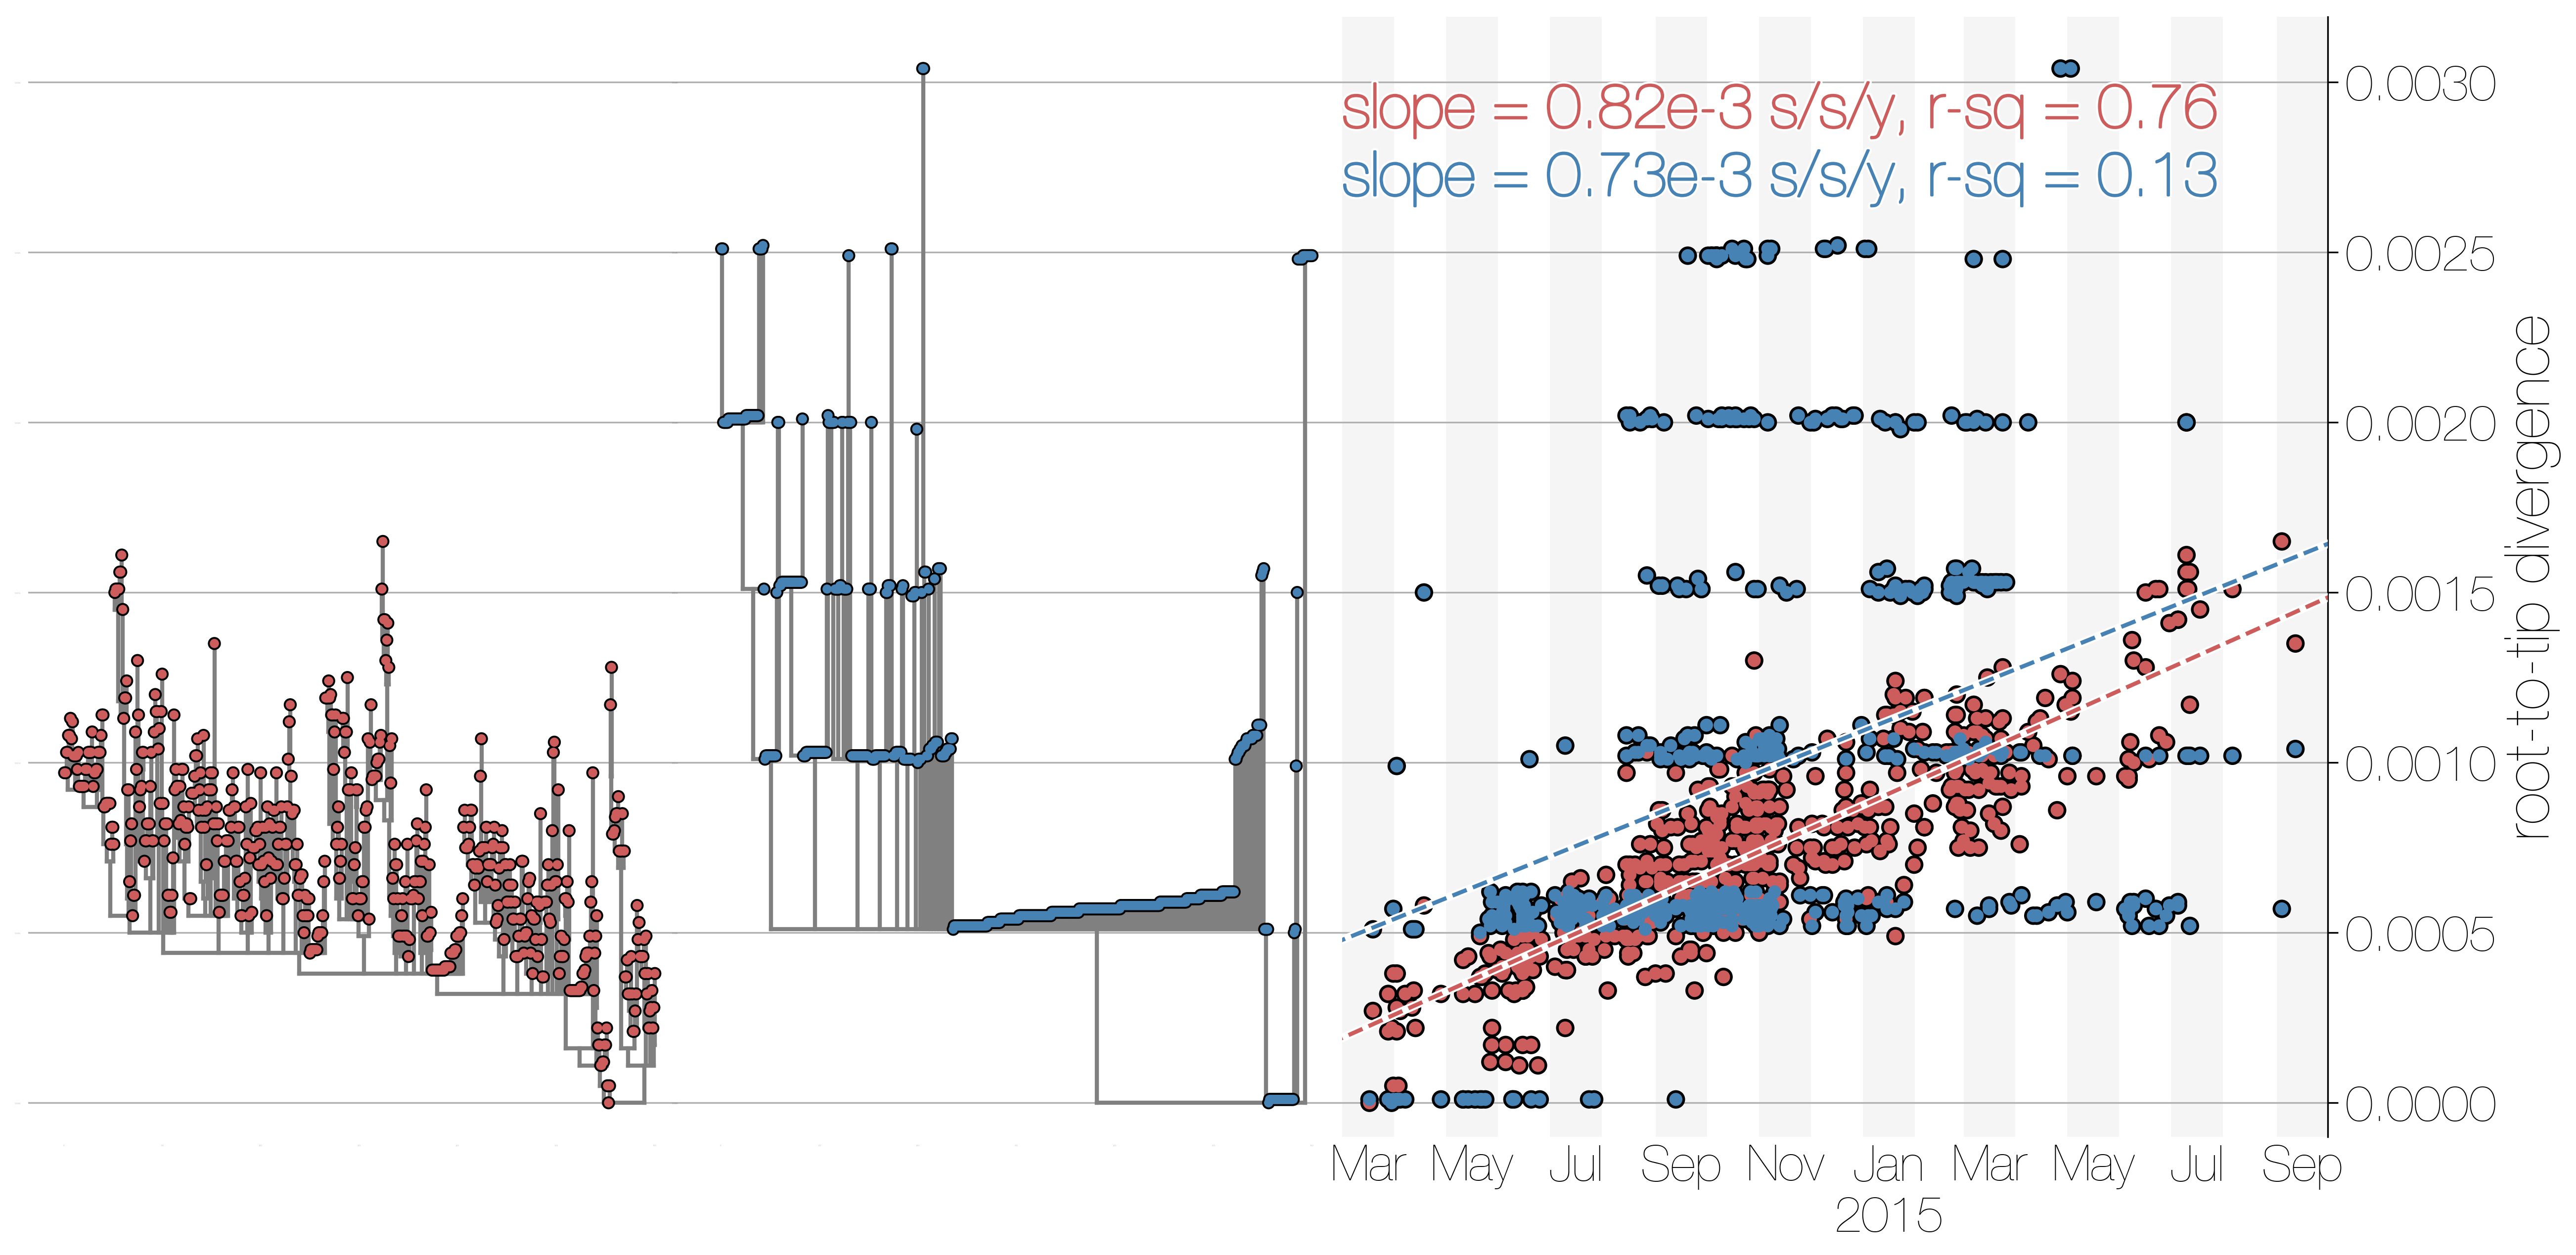
\includegraphics[width=0.75\textwidth]{supp_figures/sfigX_rtt.png}
	\caption{\textbf{Root to tip regression for maximum likelihood trees of genome (red) and GP (blue) sequences.}
  Linear regression of sequence collection dates against distance from the root gives evolutionary rate estimates (slope of the regression) at $0.82\times10^{-3}$ and $0.73\times10^{-3}$ substitutions per site per year, respectively.
  Despite similar rates the correlation between collection dates and divergence from root is far better using genomes ($r^{2}=0.76$) than GP sequences ($r^{2}=0.13$).
	}
	\label{rtt}
\end{figure}

\begin{figure}[h]
 \centering
	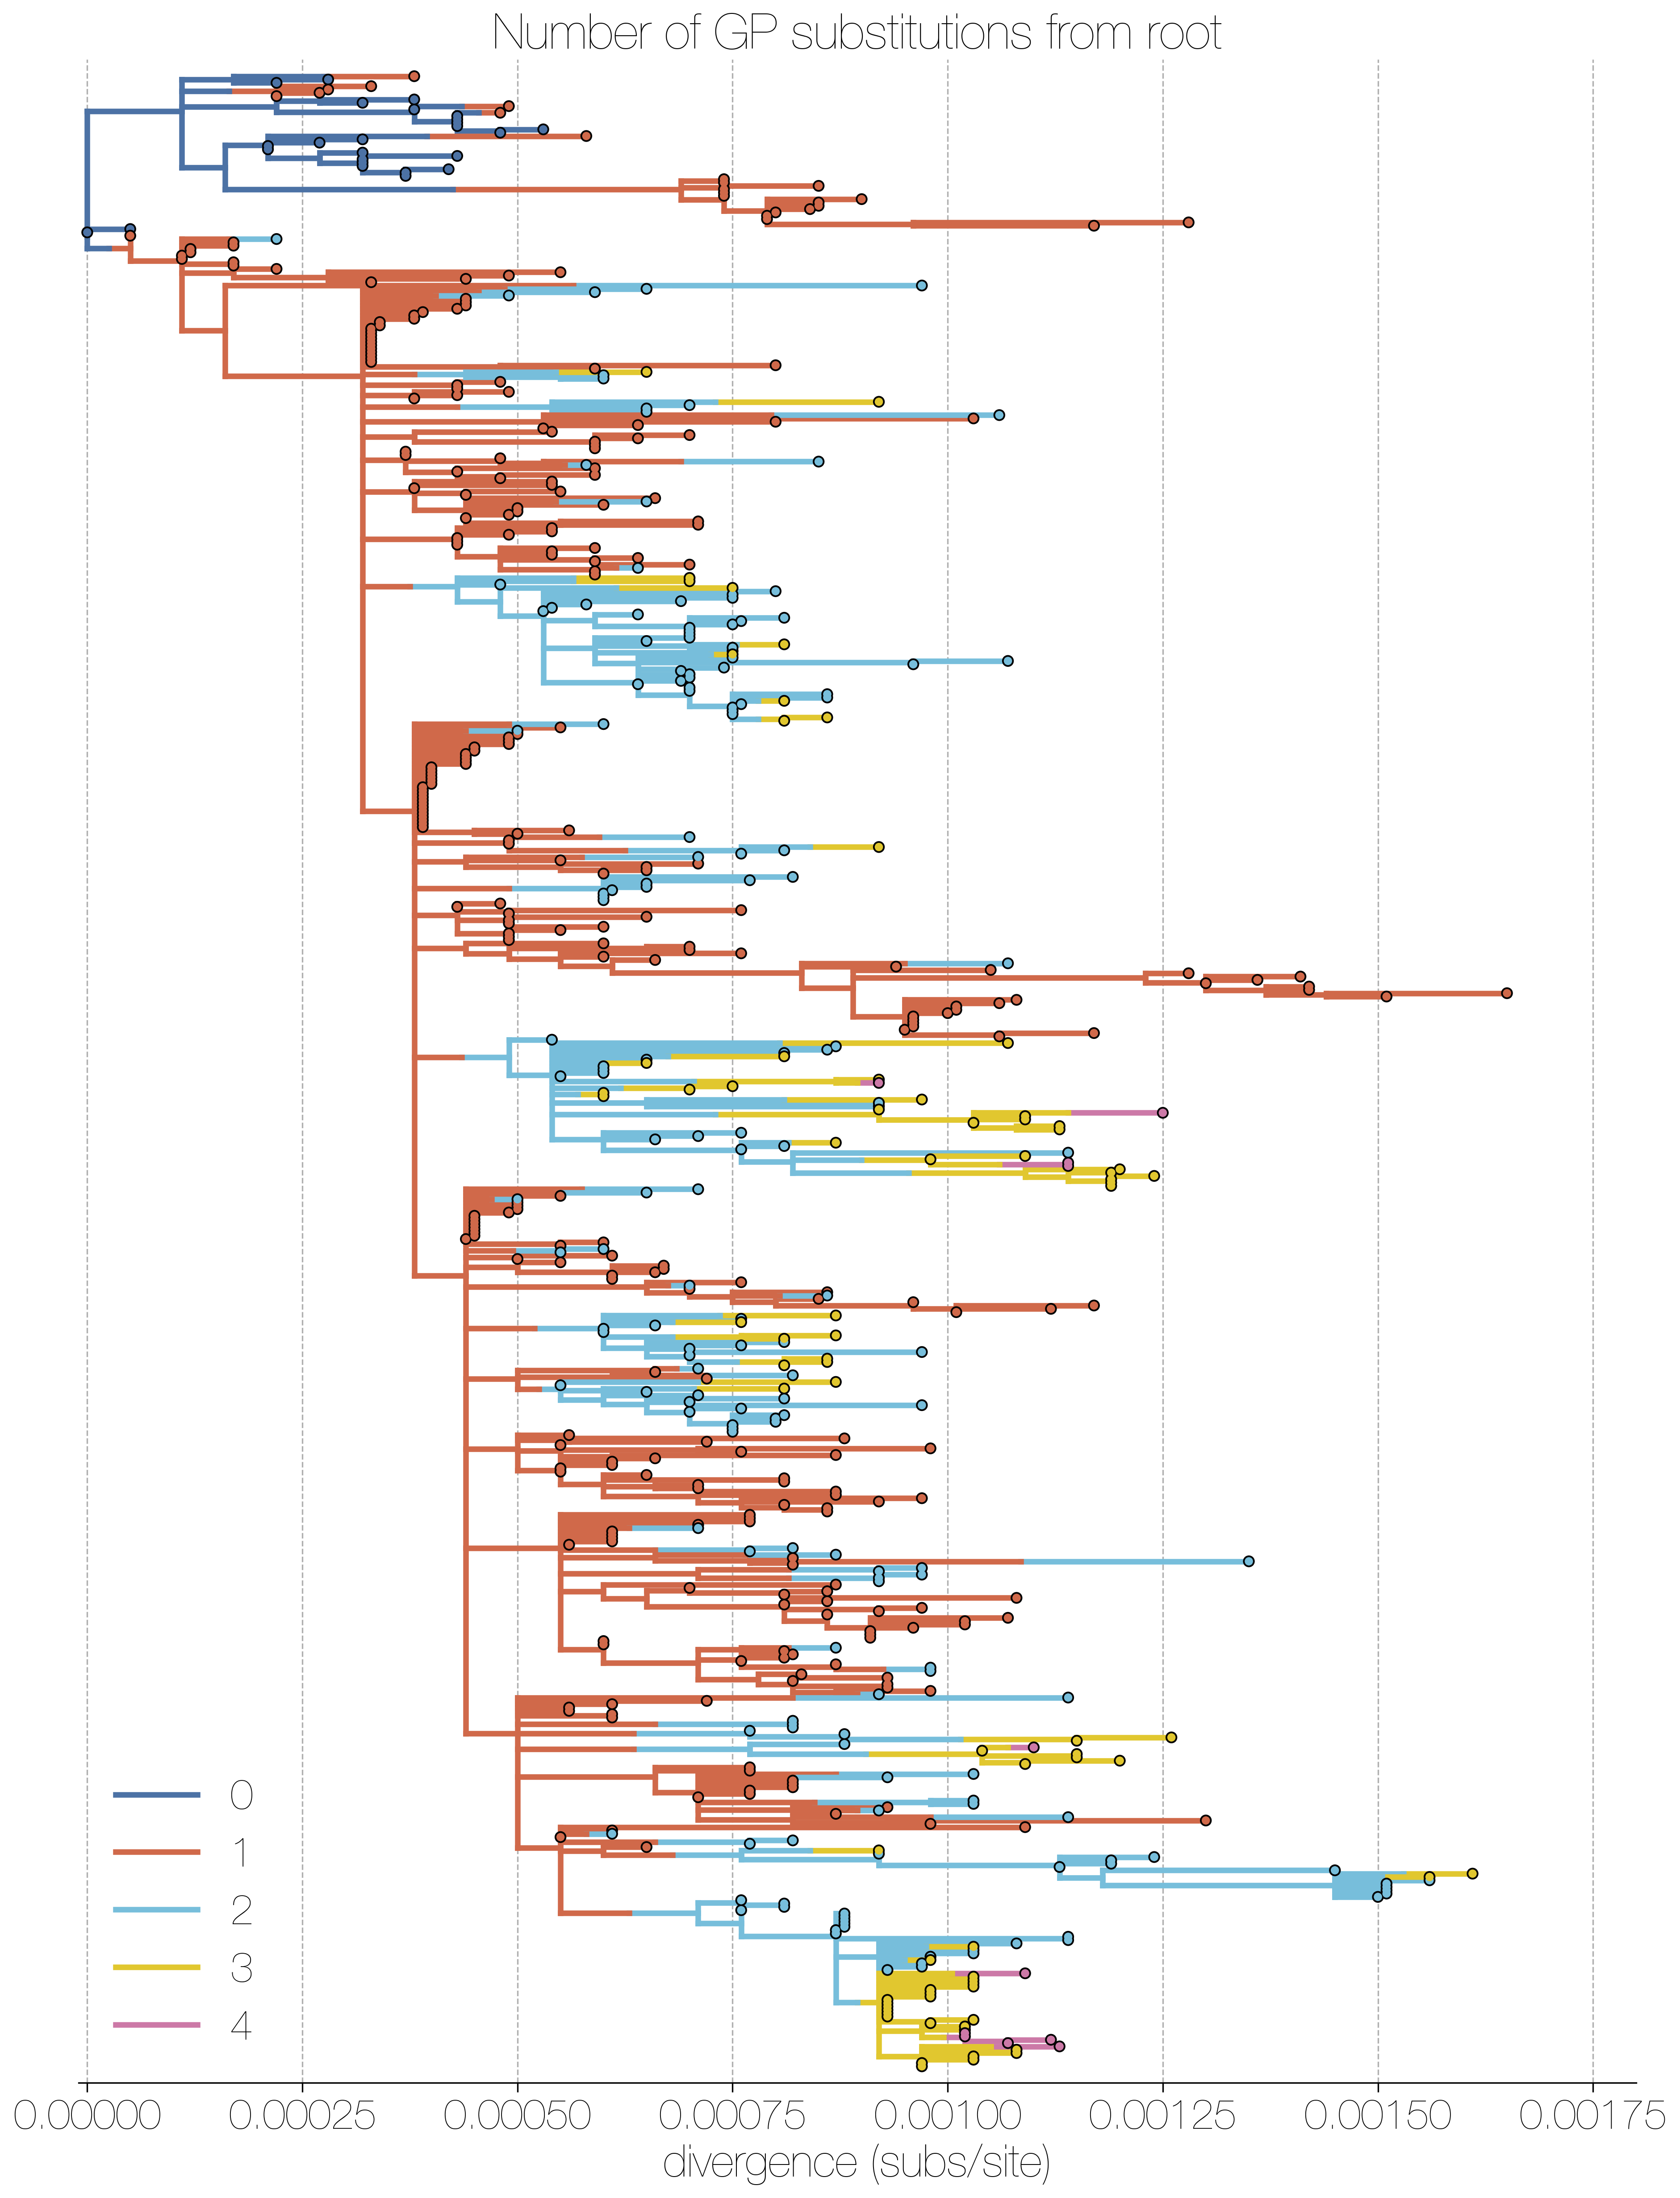
\includegraphics[width=0.75\textwidth]{supp_figures/sfigX_embedding.png}
	\caption{\textbf{Whole genome maximum likelihood tree coloured by mutations occurring in GP.}
  Colours indicate the cumulative number of mutations from the root occurring in the GP gene.
  Much of the clade resolution is lost when only considering mutations occurring in the GP gene, particularly in the already highly polytomic Sierra Leonean part of the phylogeny in red.
	}
	\label{embedding}
\end{figure}

\begin{figure}[h]
 \centering
	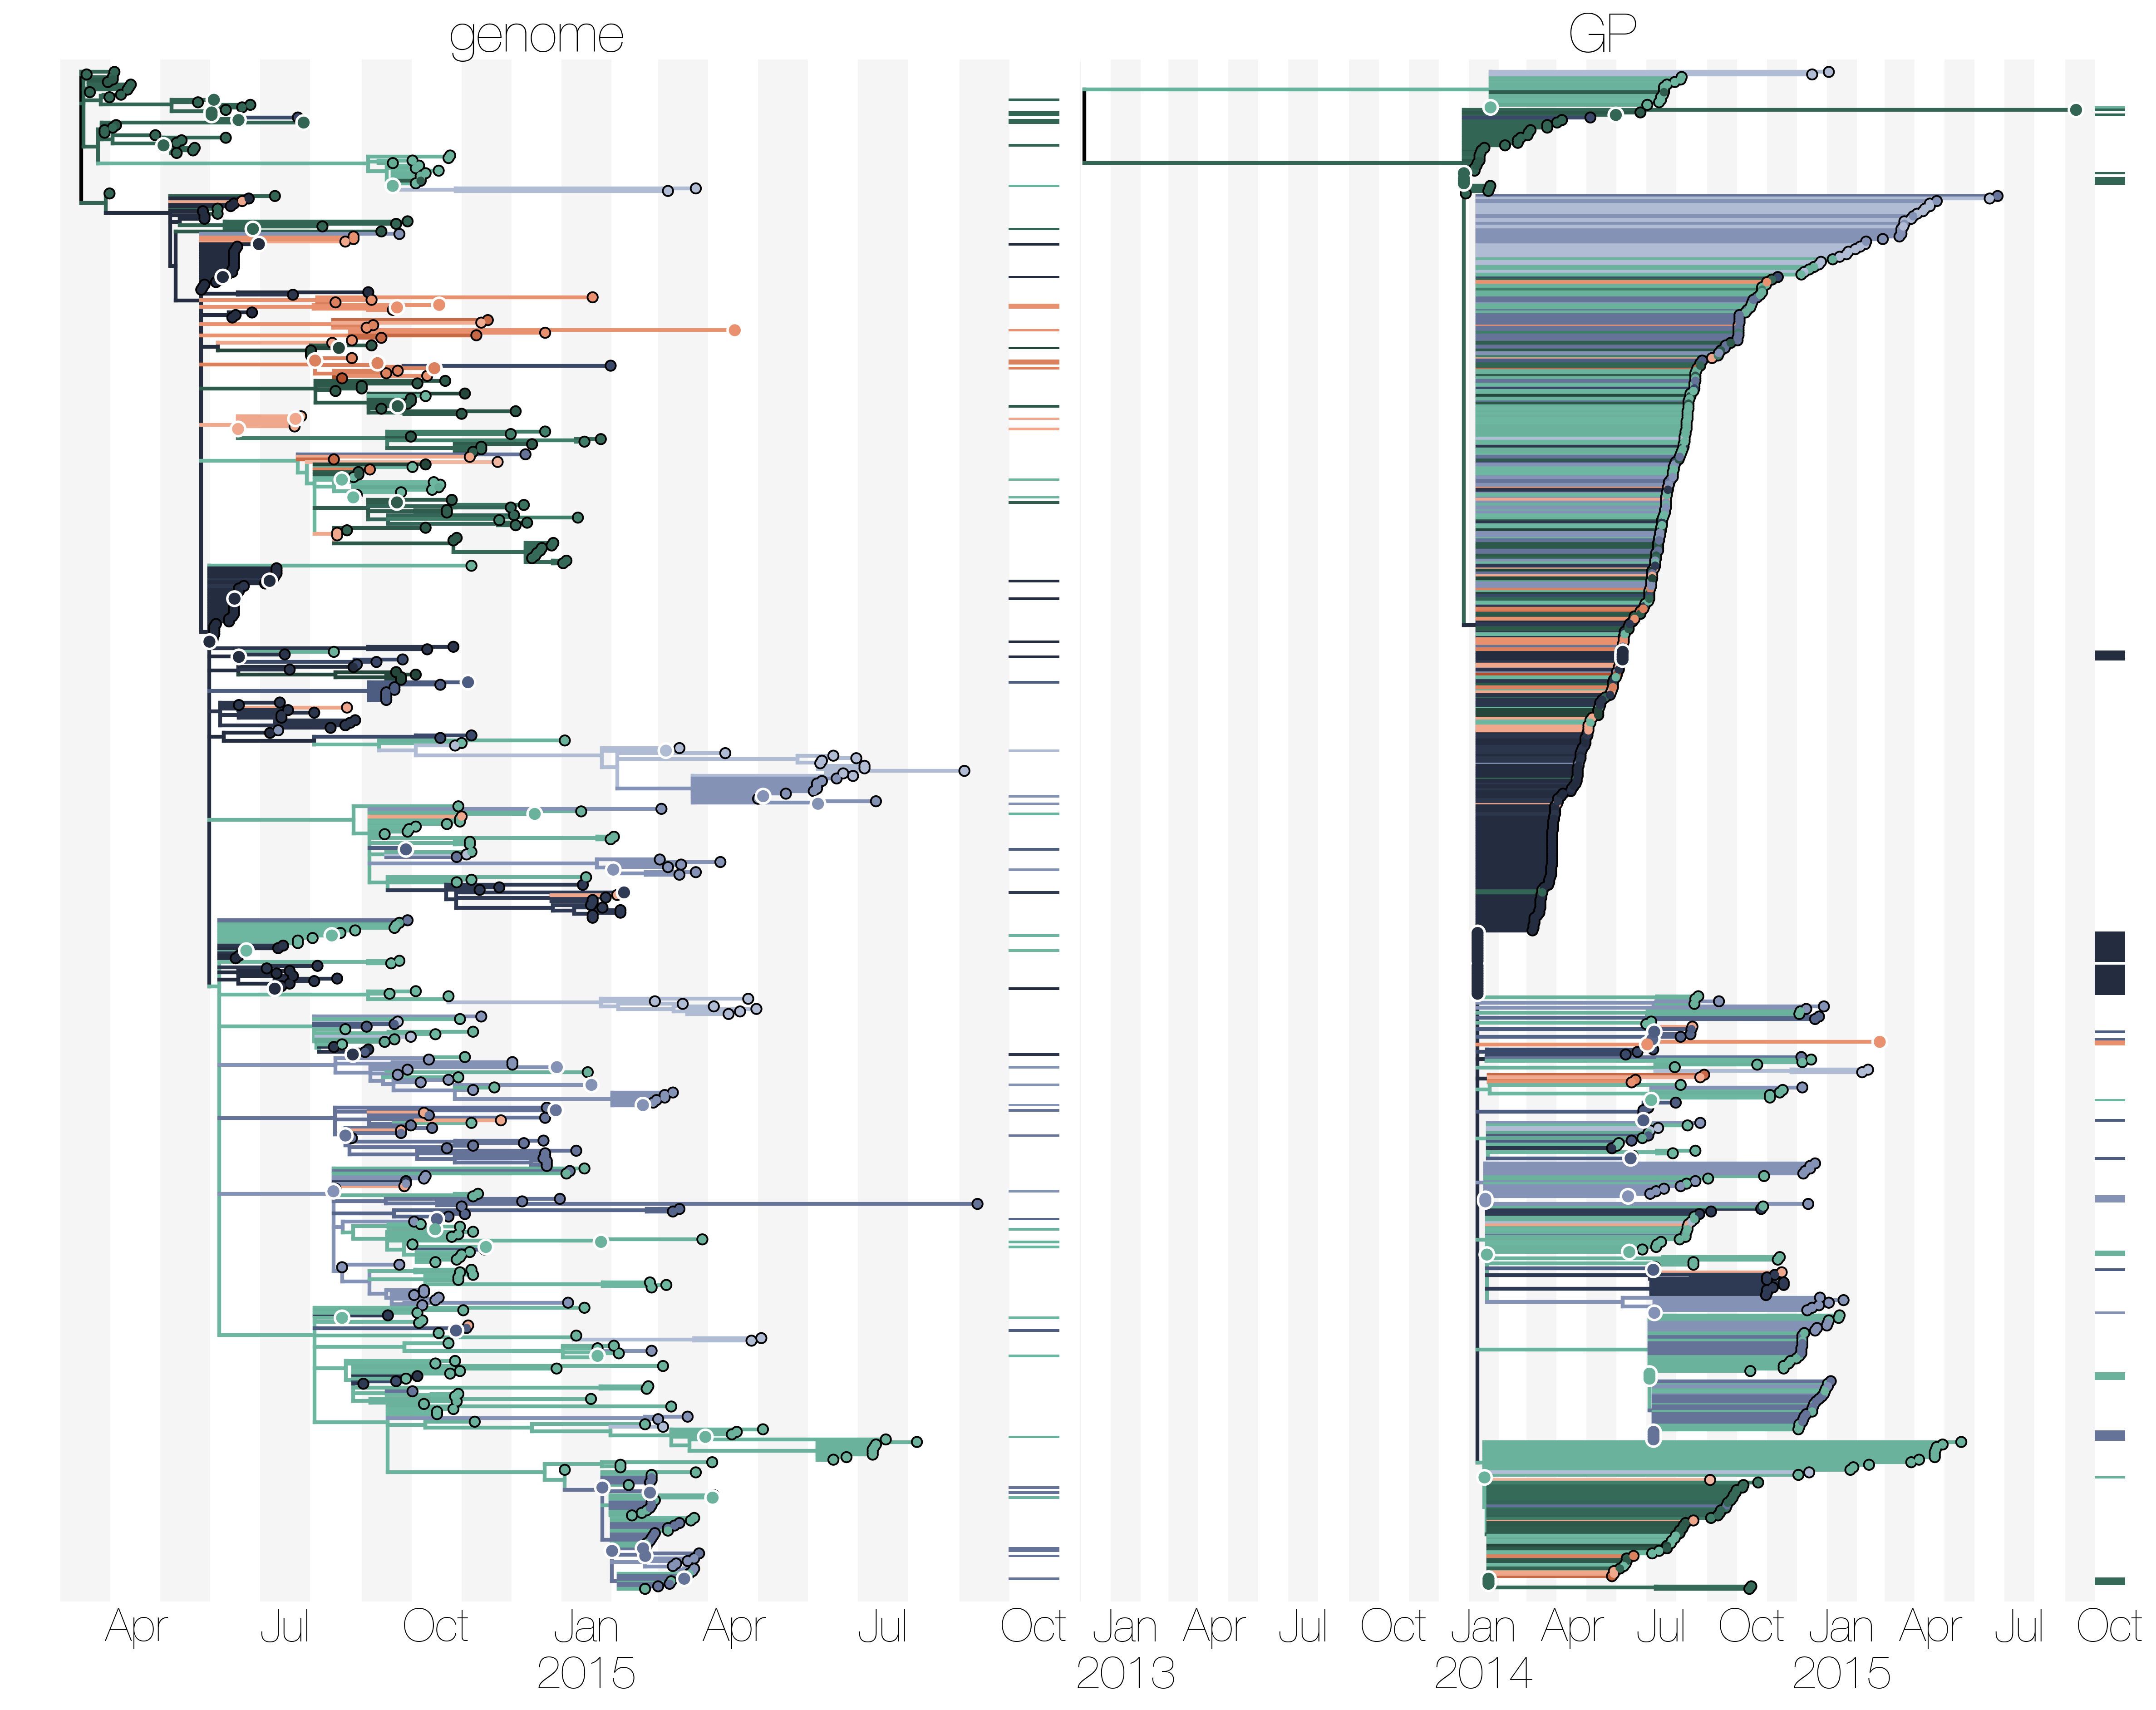
\includegraphics[width=0.75\textwidth]{supp_figures/sfigX_treetimeTrees.png}
	\caption{\textbf{Maximum likelihood phylogeny of complete Ebola virus genomes coloured by mutations occurring within the coding sequence of GP.}
  GP sequences are too short to capture many of the mutations that could differentiate both large scale features, \textit{e.g.} Sierra Leone backbone in red, as well as smaller clades.
	}
	\label{TTtrees}
\end{figure}

\begin{figure}[h]
 \centering
	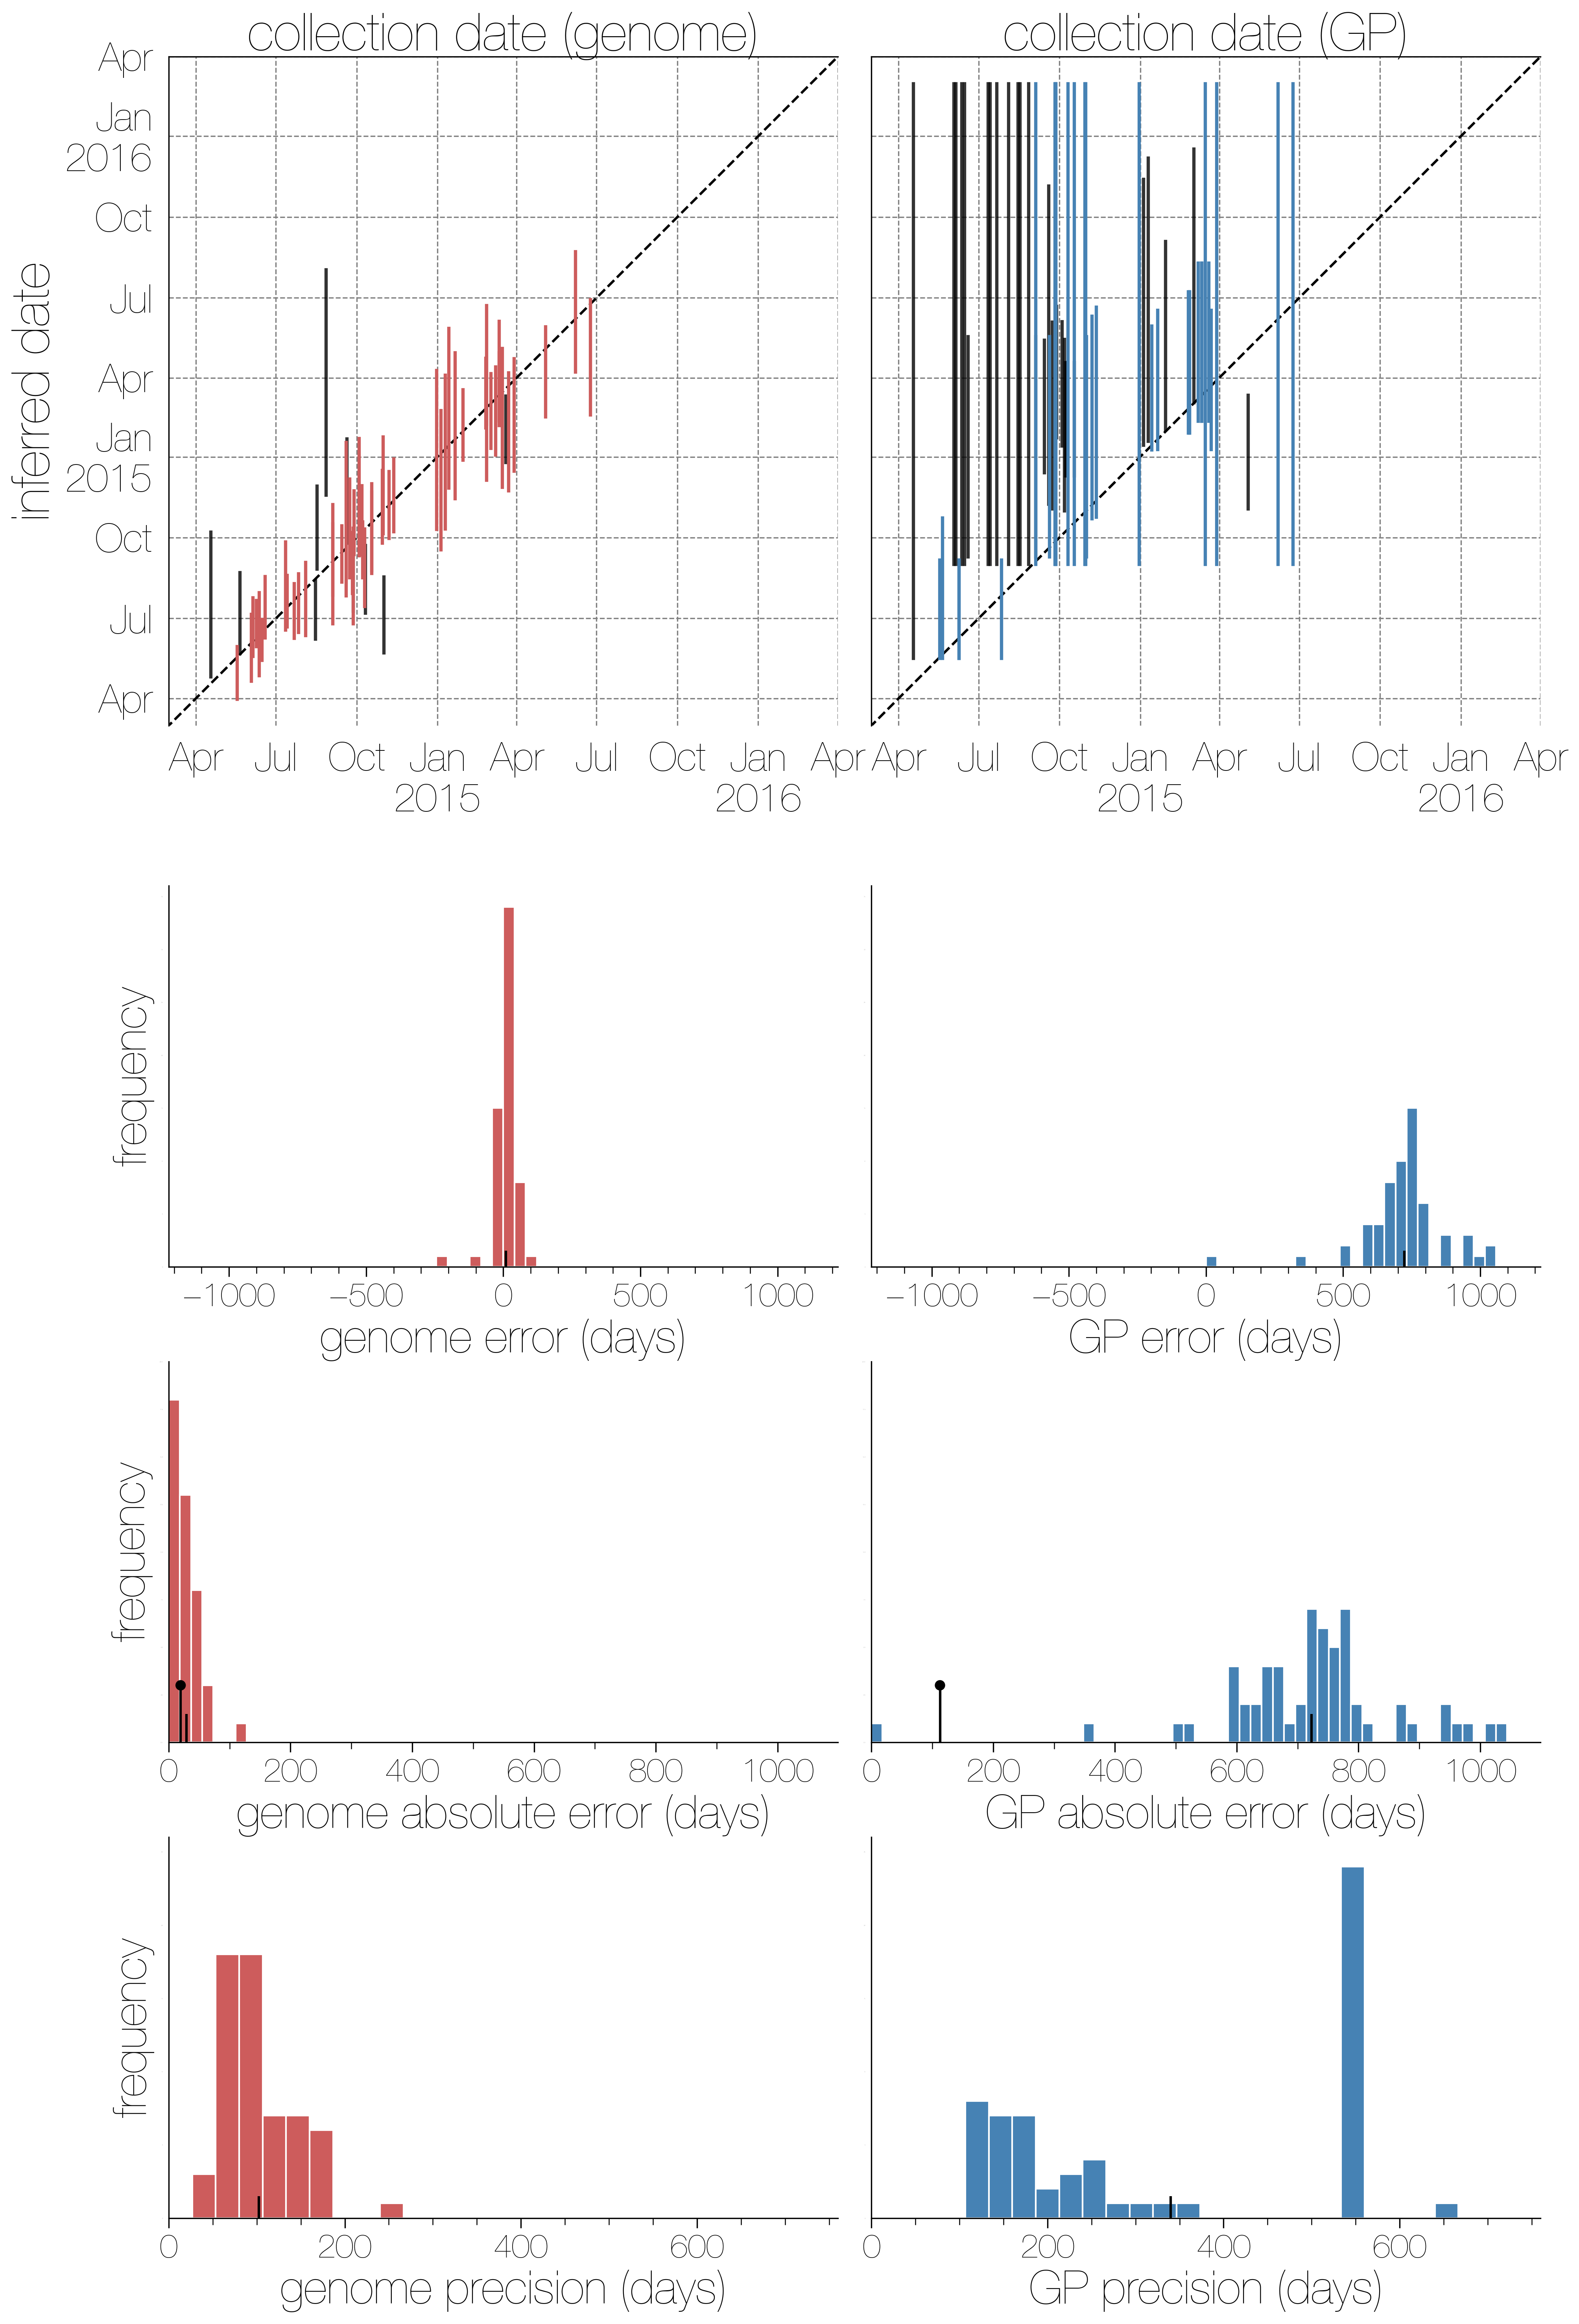
\includegraphics[width=0.75\textwidth]{supp_figures/sfigX_treetimeDates.png}
	\caption{\textbf{Maximum likelihood inference of masked tip dates from genomes (red, left) and GP sequences (blue, right) using TreeTime.}
  Vertical bars indicate the 95\% confidence interval for marginal reconstruction of masked tip dates plotted against their true dates.
  Tip dates where the 95\% confidence interval excludes the true value are shown in black.
	}
	\label{TTdates}
\end{figure}

\begin{figure}[h]
 \centering
	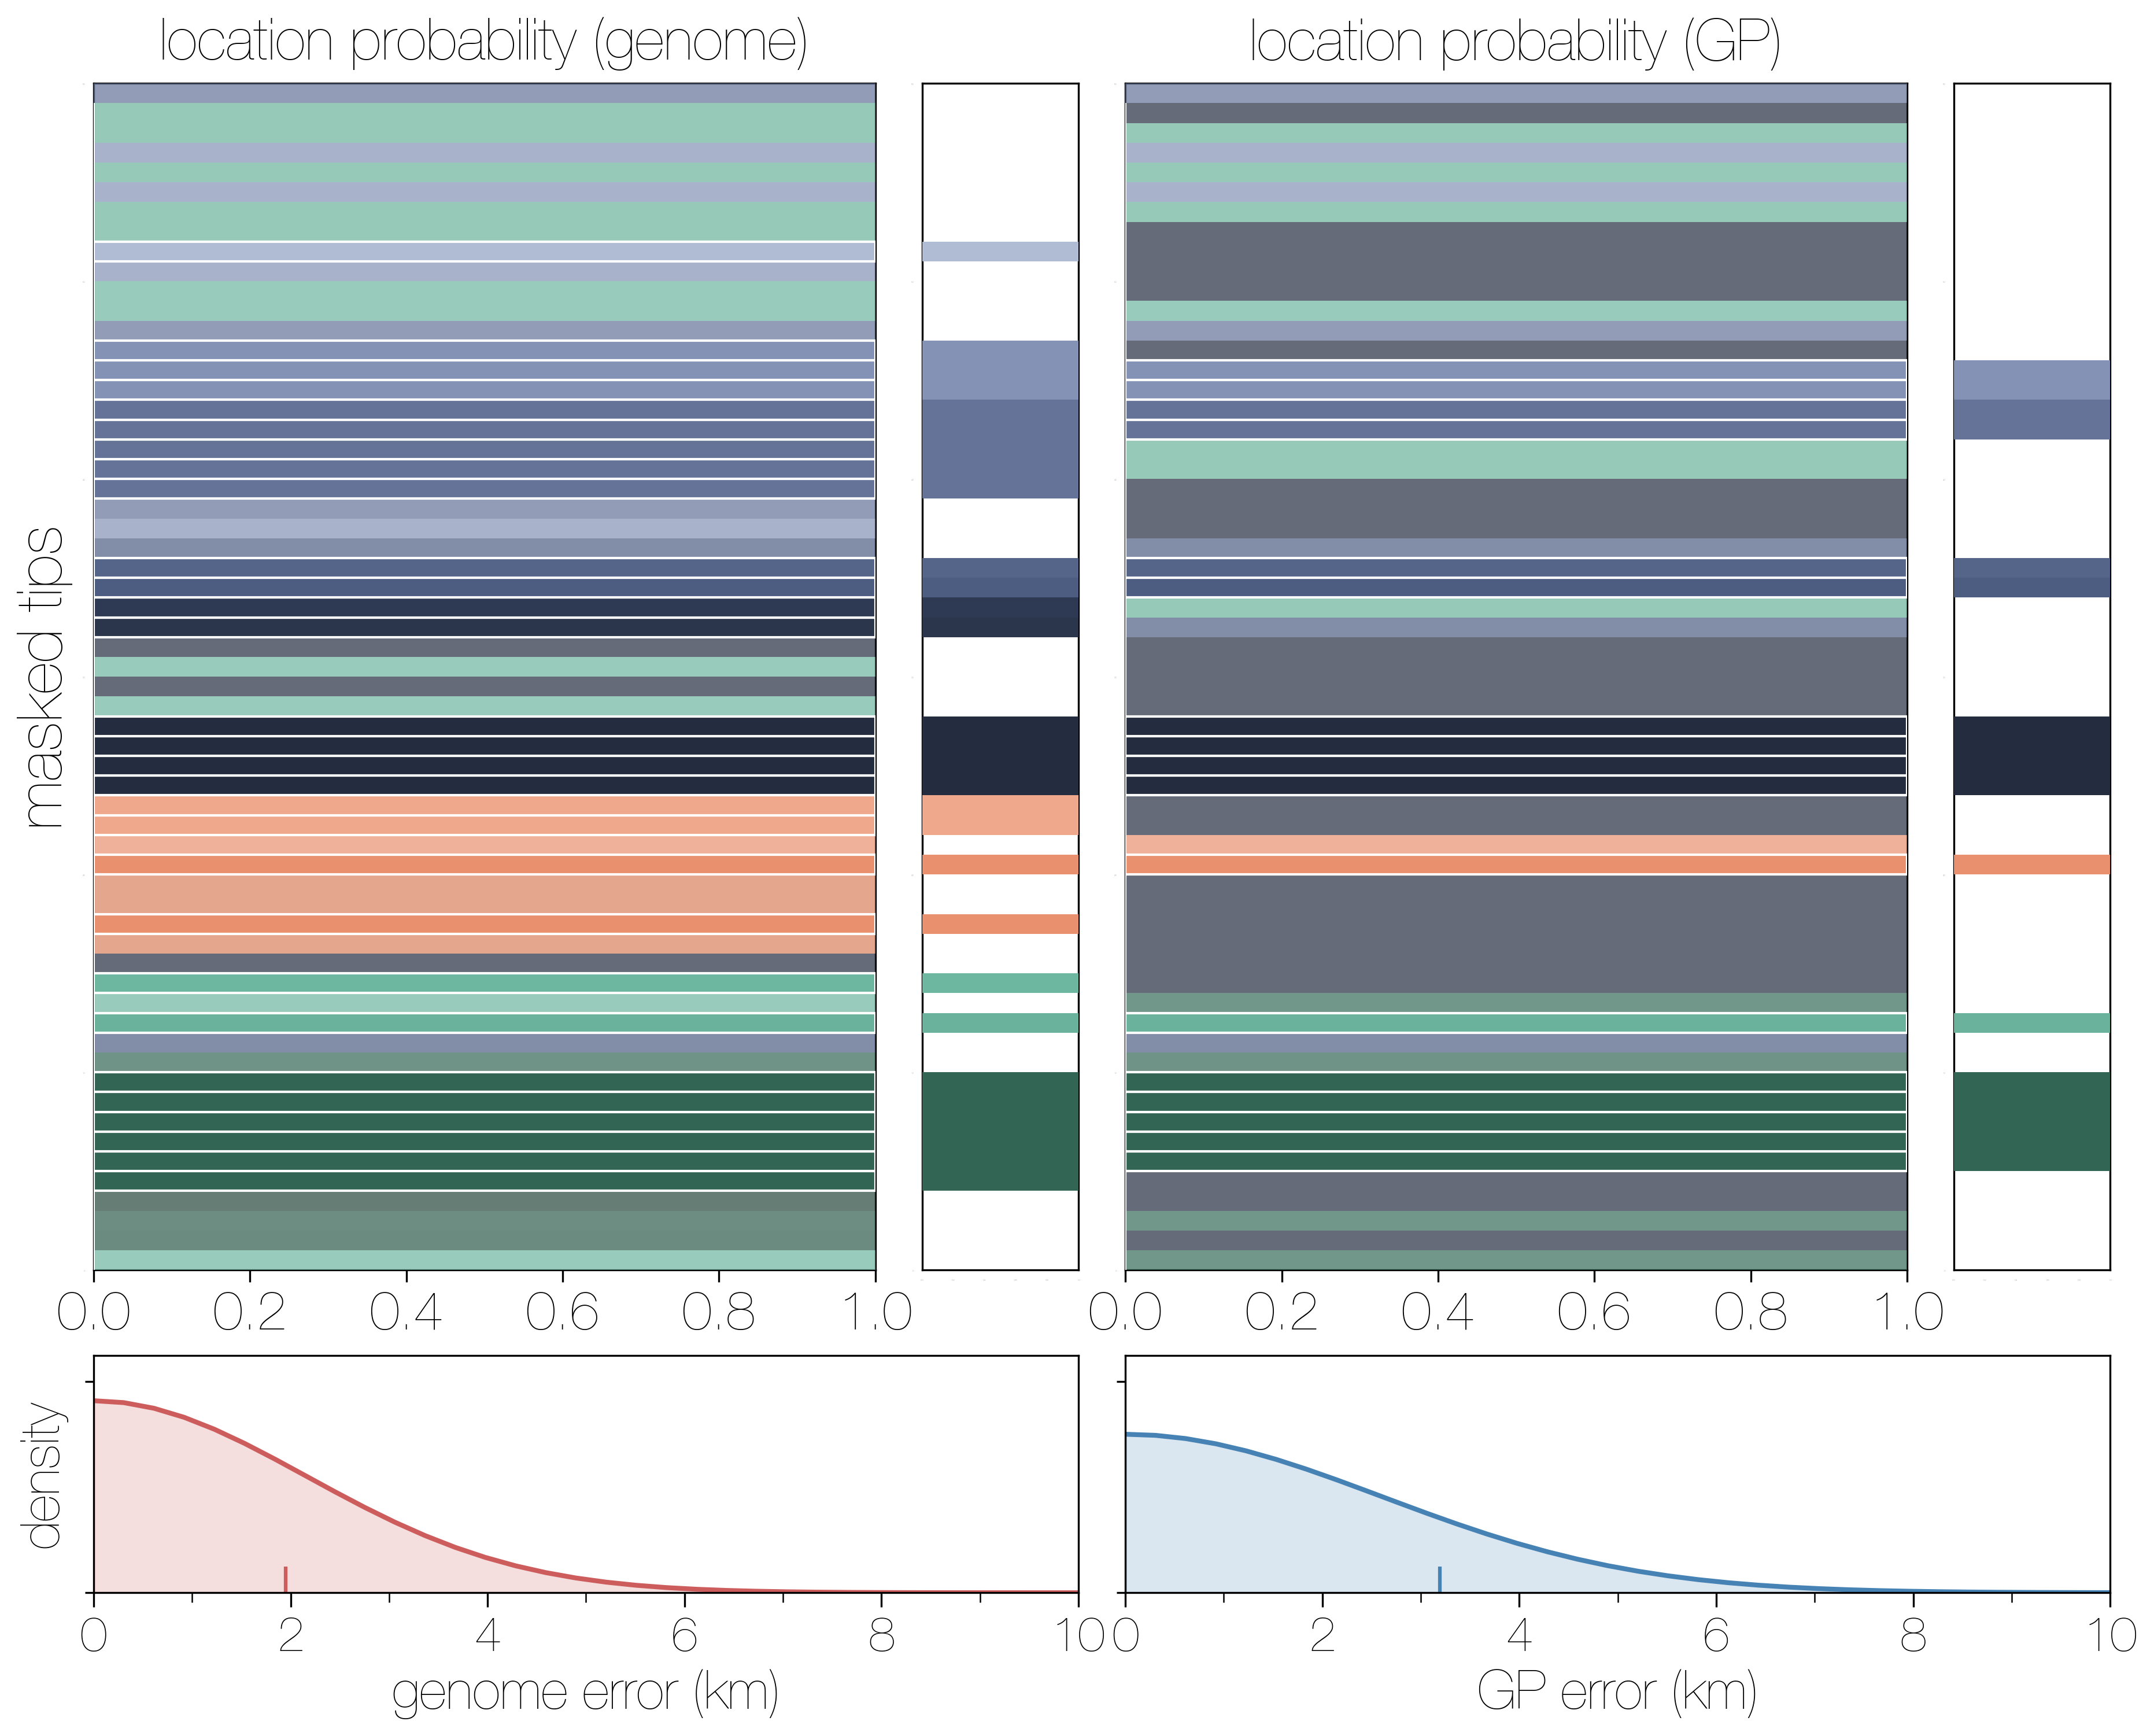
\includegraphics[width=0.75\textwidth]{supp_figures/sfigX_treetimeLocations.png}
	\caption{\textbf{Maximum likelihood inference of masked sequence location from genomes (left) and GP sequences (right) via a CTMC model implemented in TreeTime.}
  Unlike the Bayesian GLM where probabilities are spread across different locations, the CTMC gives categorical support to one location.
  Genomes still perform better in terms of correct guess (29/60 for genomes versus 17 for GP), cross entropy (23126.93 for genome versus 32079.48 for GP) and mean probability-weighted great circle distance between true location population centroid and estimated location population centroid (1.95 km for genome versus 3.19 for GP).
	}
	\label{TTlocations}
\end{figure}

\begin{figure}[h]
 \centering
  \subfloat{
  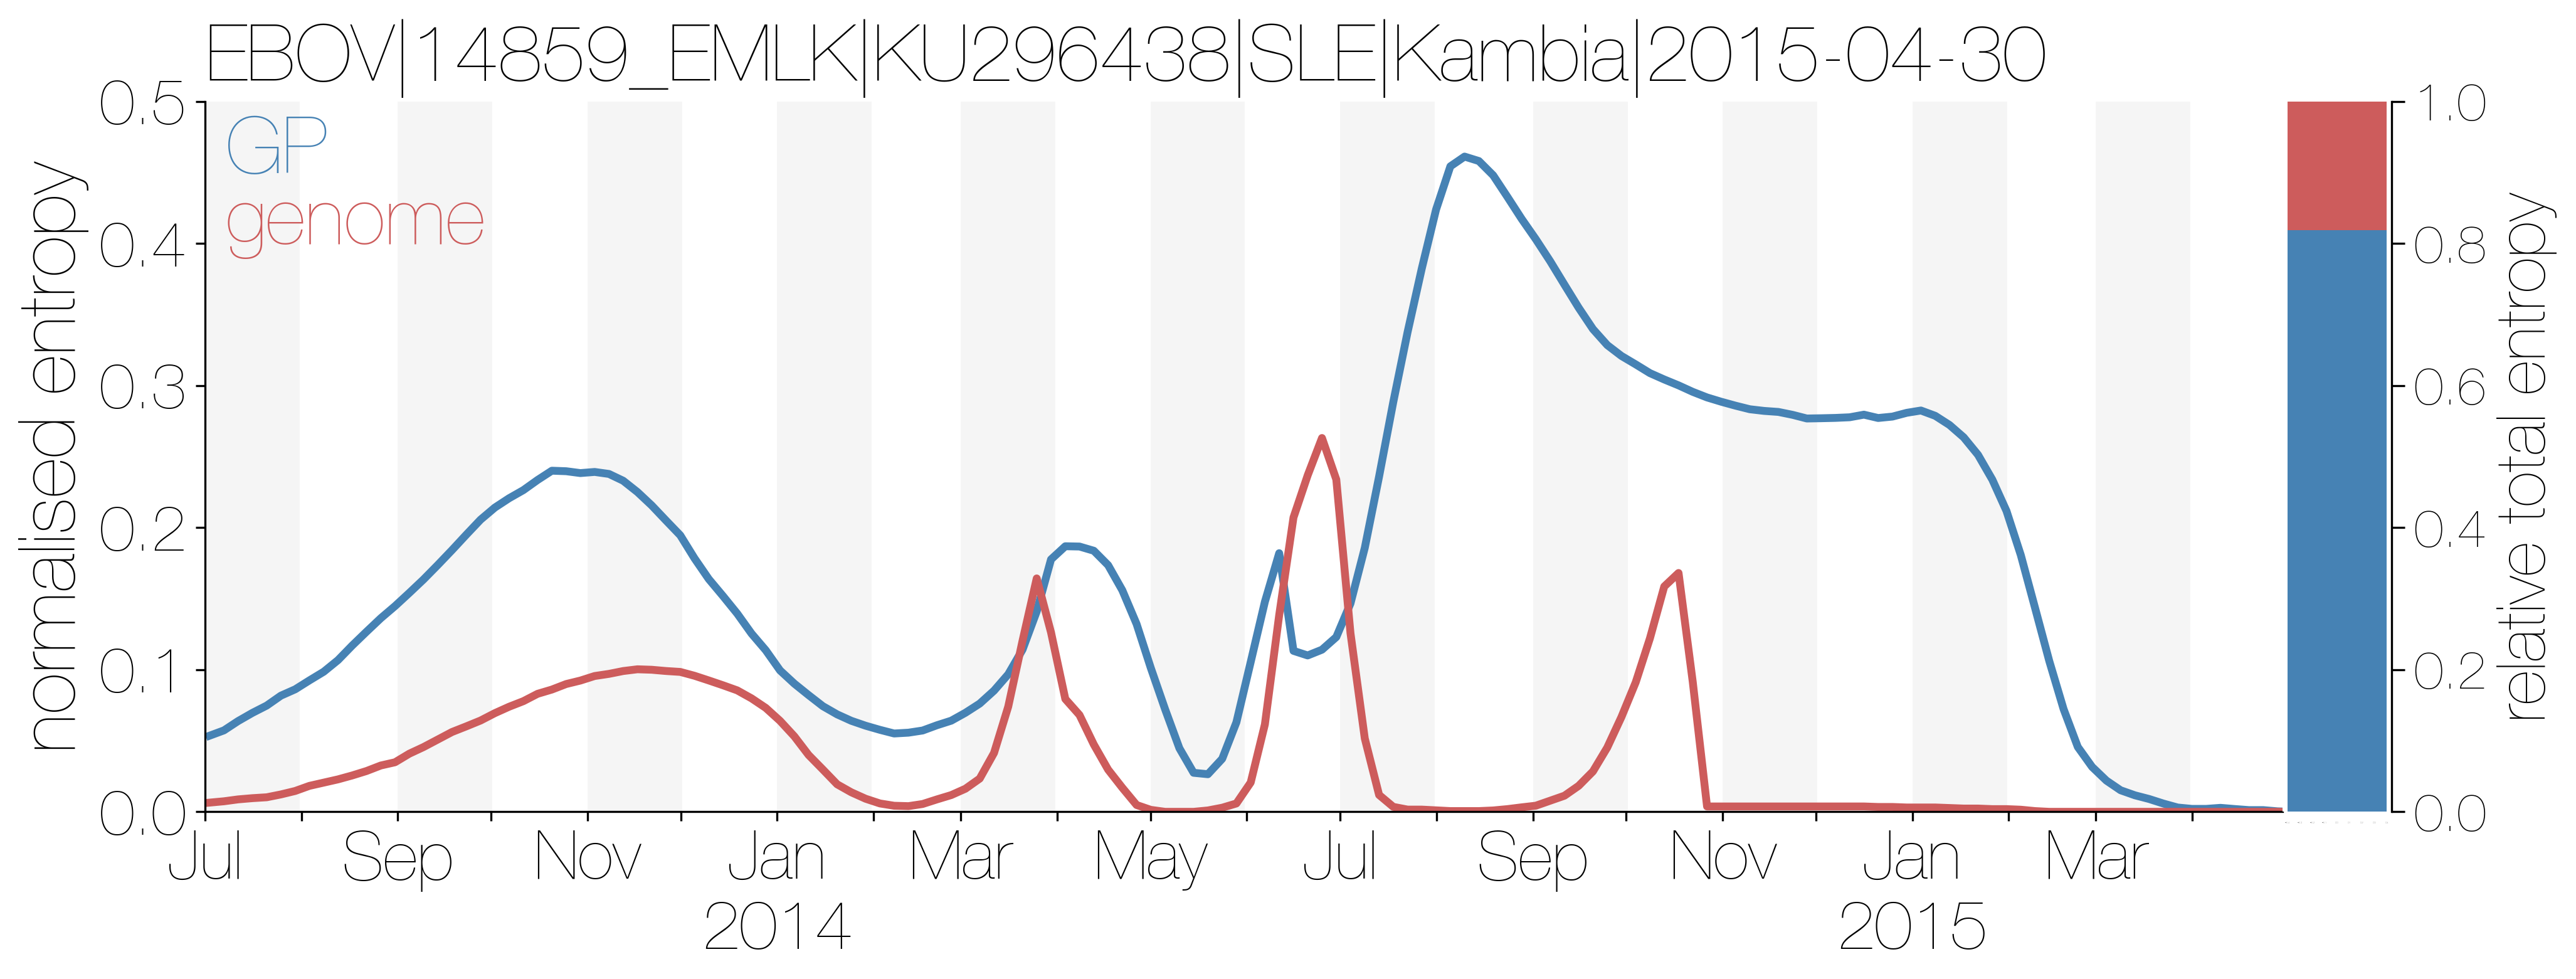
\includegraphics[width=0.45\textwidth]{supp_figures/sfigXA_locationEntropy.png}
  }
  \subfloat{
  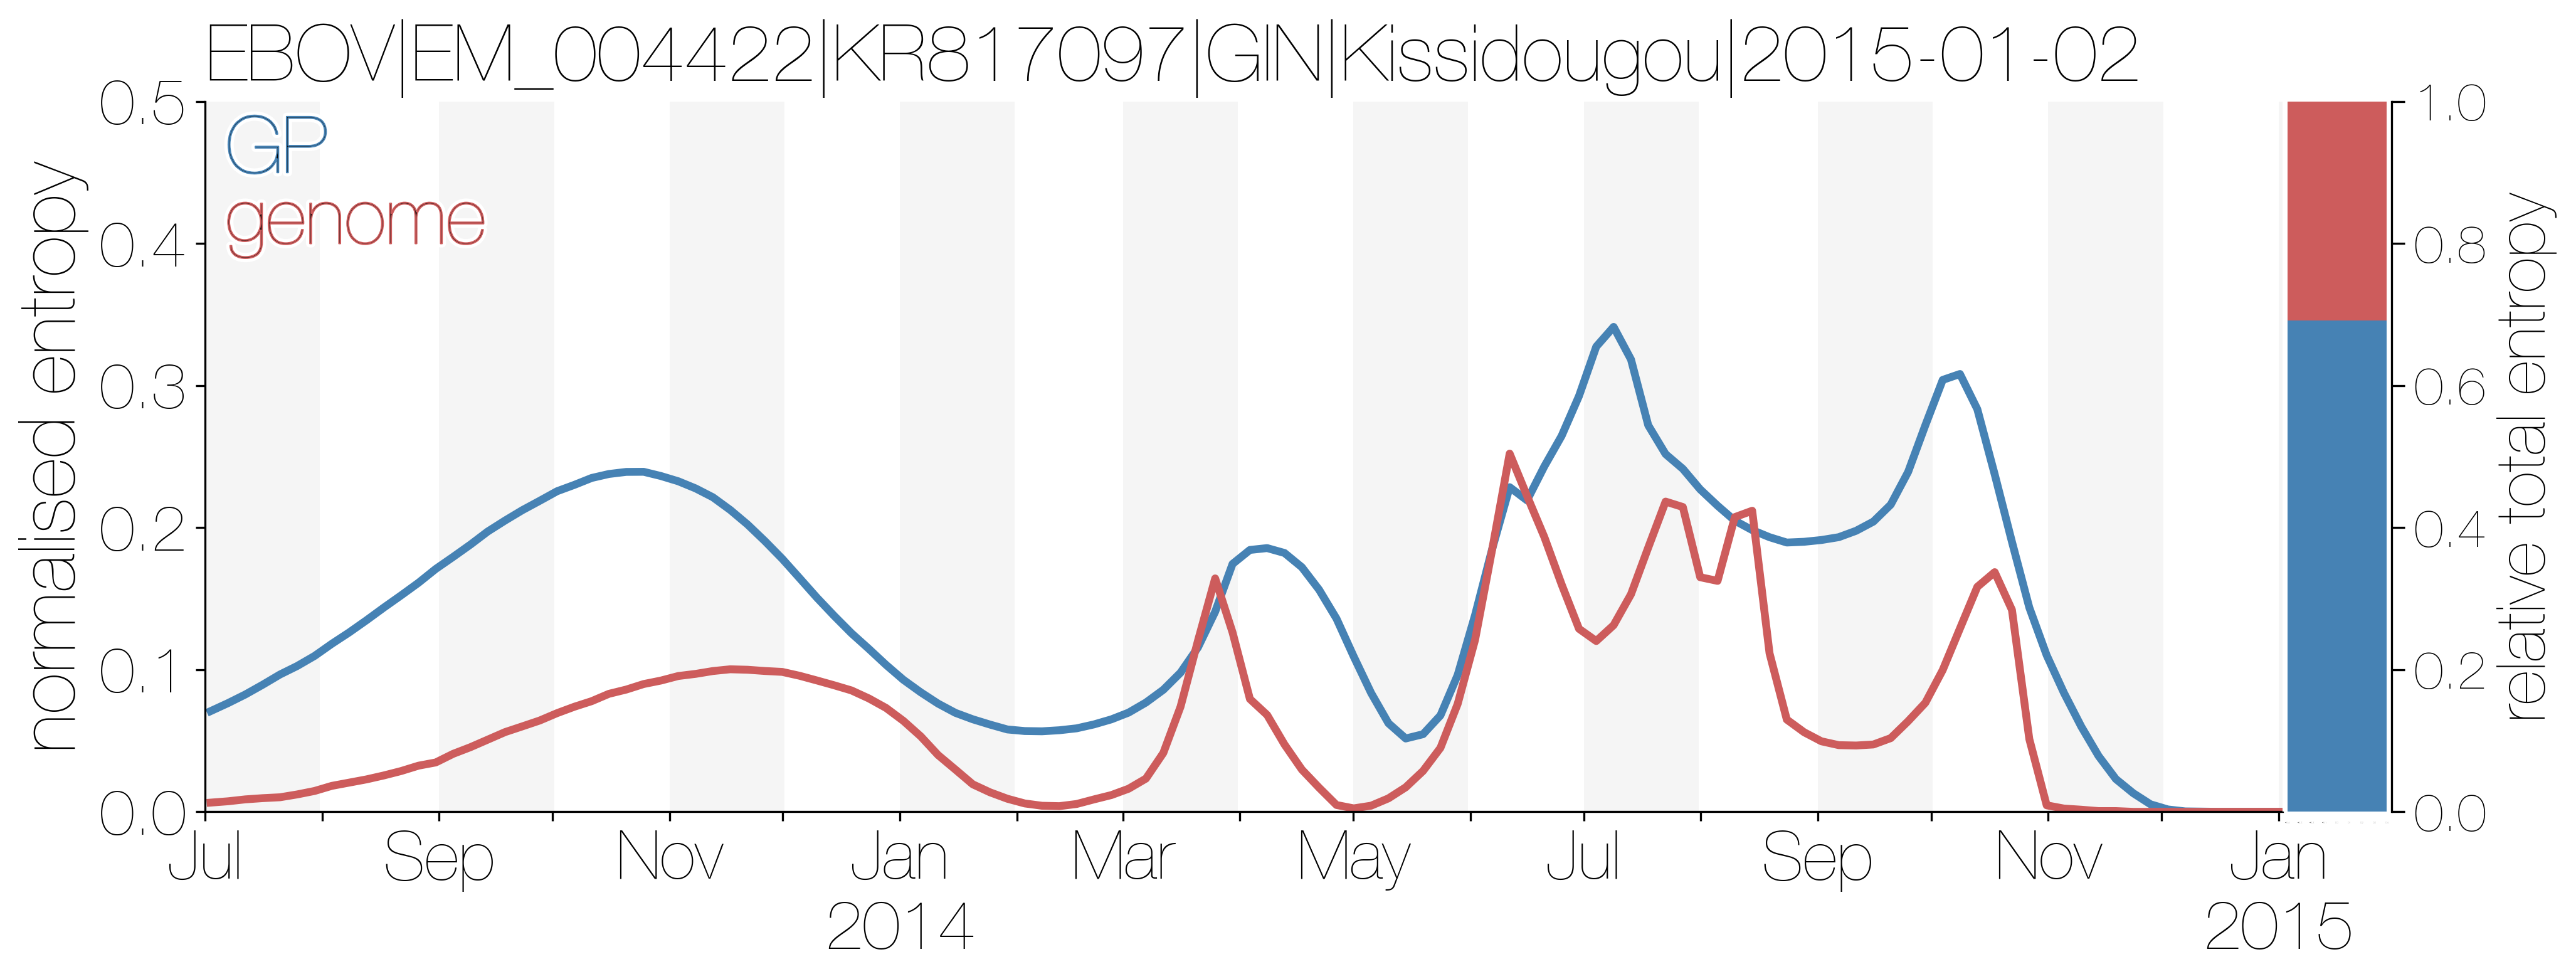
\includegraphics[width=0.45\textwidth]{supp_figures/sfigXB_locationEntropy.png}
  }
  \\
  \subfloat{
  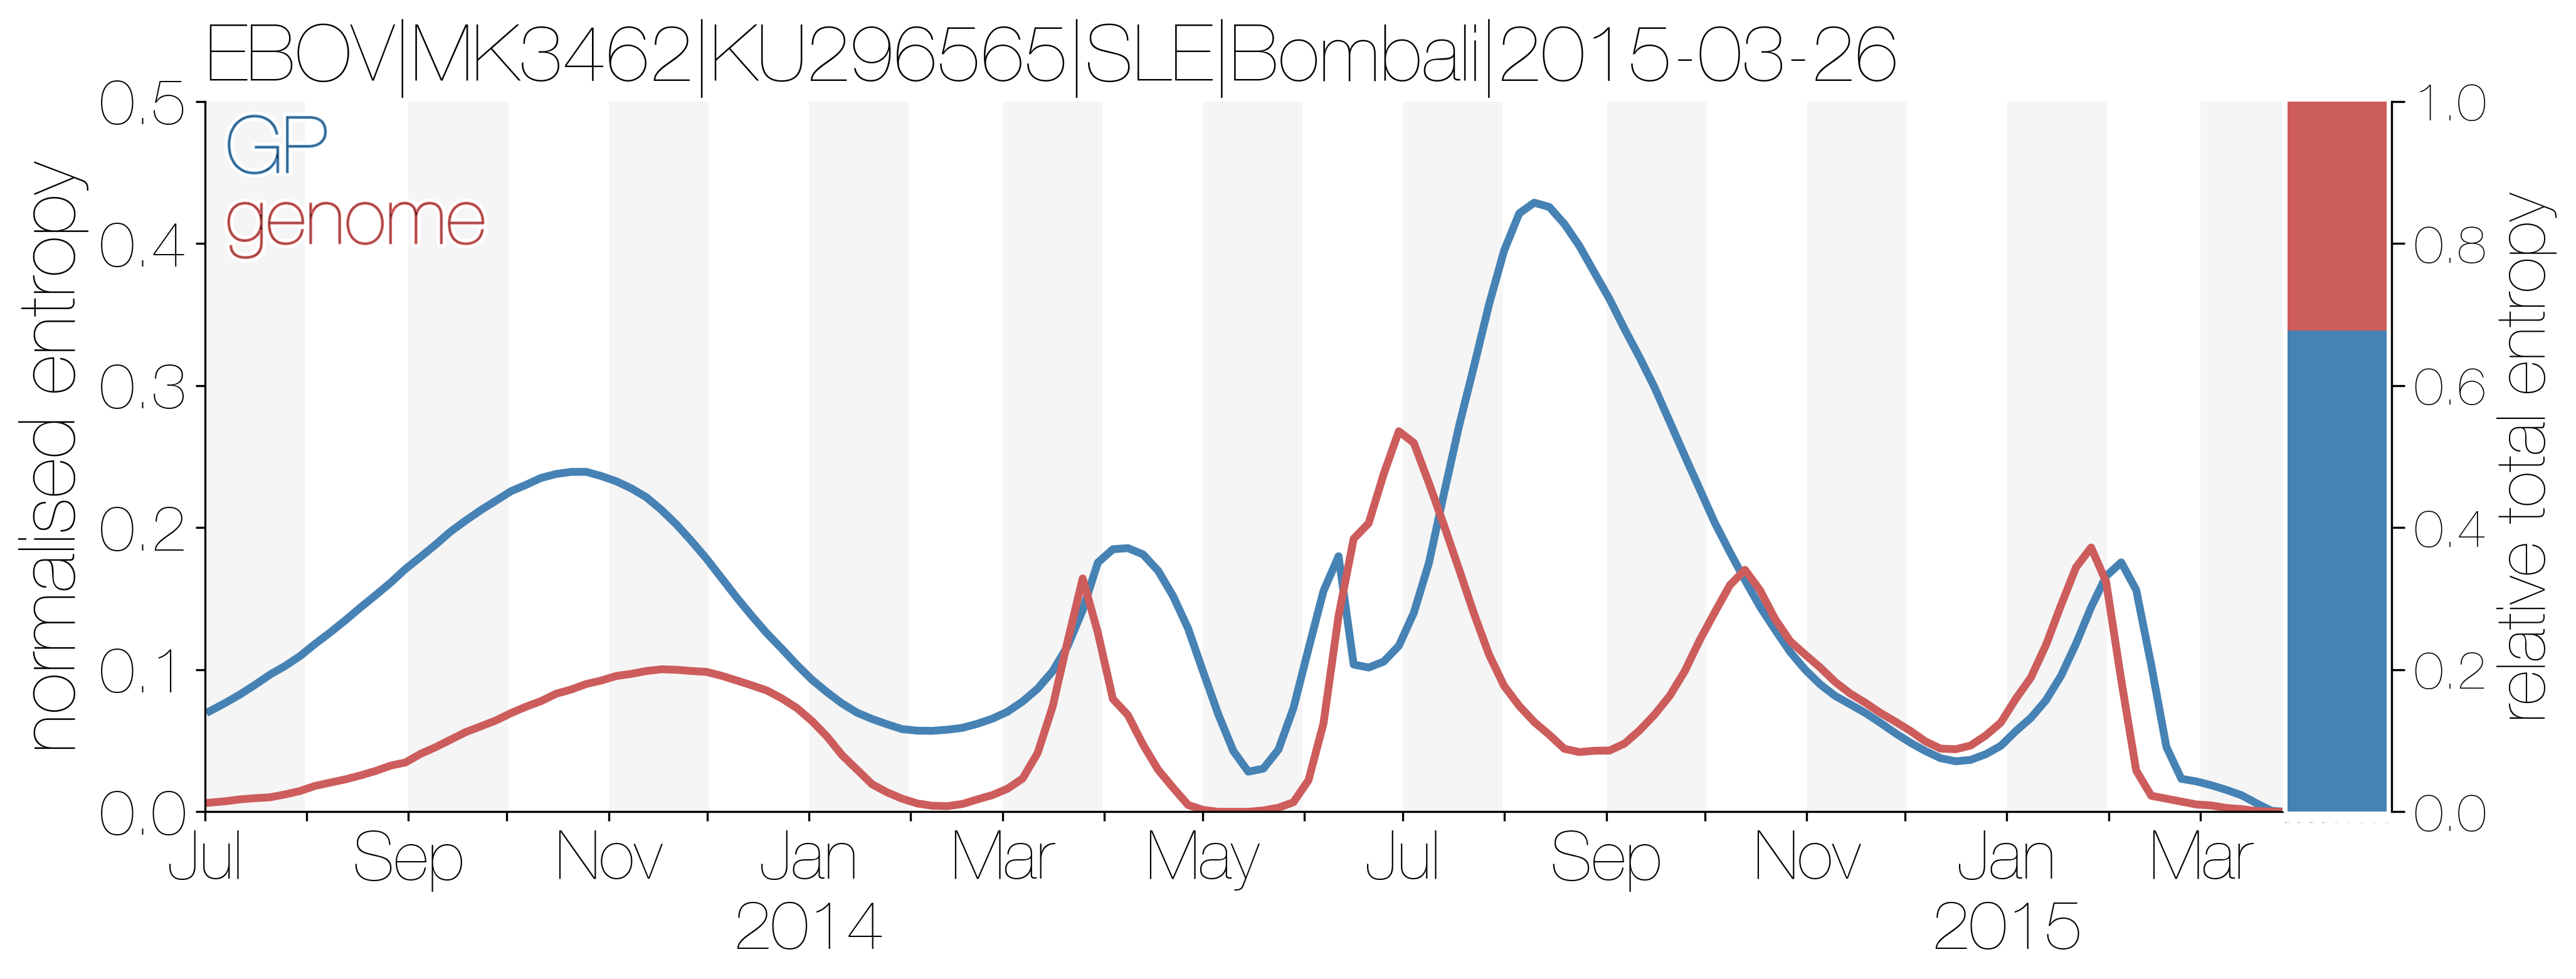
\includegraphics[width=0.45\textwidth]{supp_figures/sfigXC_locationEntropy.png}
  }
  \subfloat{
  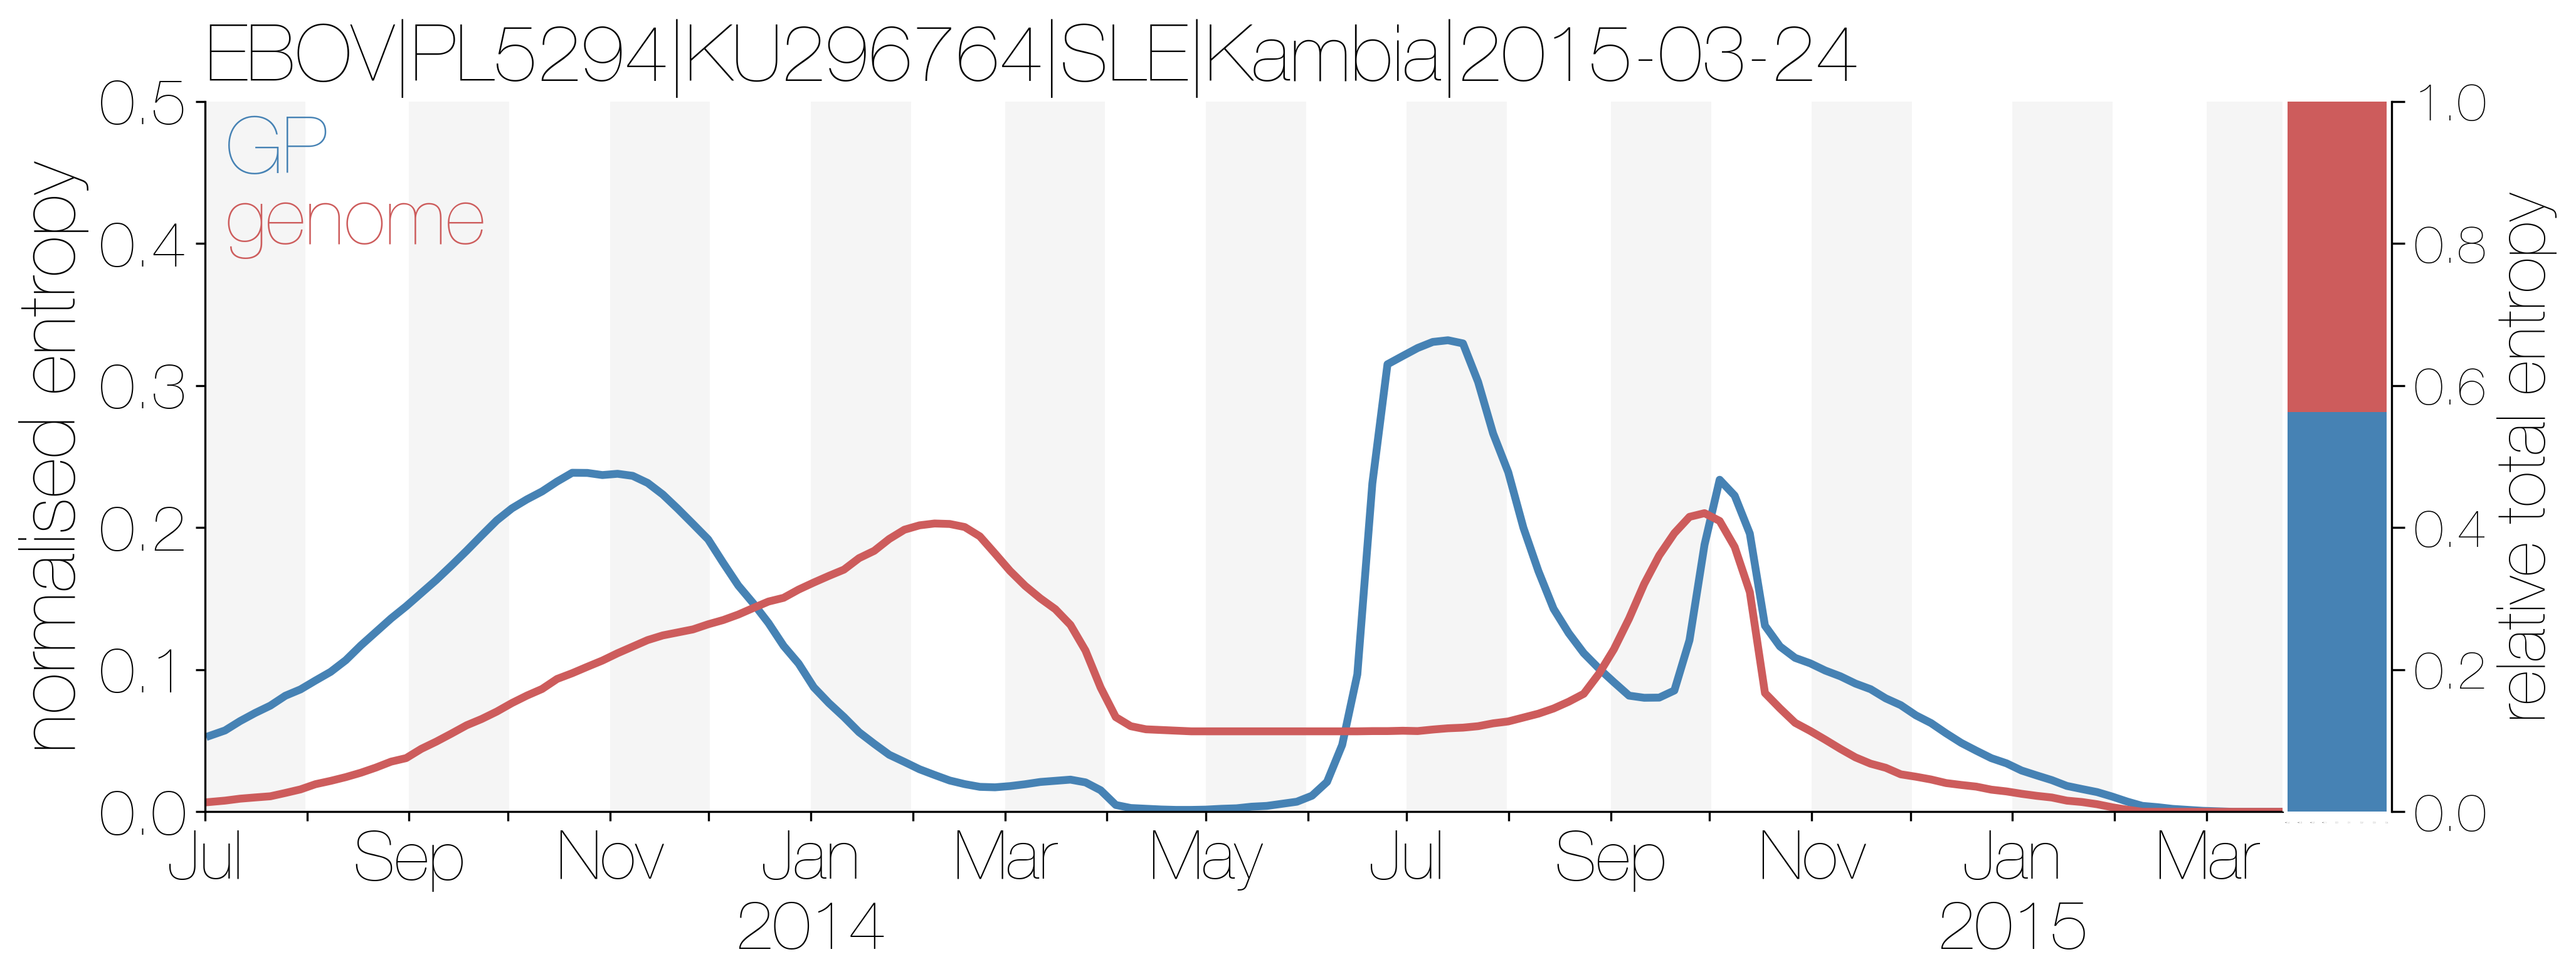
\includegraphics[width=0.45\textwidth]{supp_figures/sfigXD_locationEntropy.png}
  }
  \caption{\textbf{Entropies of posterior ancestral location reconstruction from genomes (red) and GP sequences (blue) for four tips.}
  Ancestral state reconstructions from genomes typically have lower entropies relative to reconstructions derived from GP sequences, indicating better certainty in location assignment at any given time.
  Red and blue bars at the end of the plot indicate relative cumulative entropies of genome and GP sequence reconstructions, respectively.
  }
	\label{trace_entropy}
\end{figure}

\end{document}
